\documentclass[a4paper, 11pt]{memoir}

% Nécessaire
\usepackage[utf8]{inputenc}
\usepackage[T1]{fontenc}
\usepackage{lmodern}

% Biblio
\usepackage{natbib}
\bibliographystyle{abbrvnat}
\usepackage{hypernat}
\bibpunct{\textcolor{blue}{[}}{\textcolor{blue}{]}}{\textcolor{blue}{;}}{a}{\textcolor{blue}{,}}{;}

\usepackage[french]{babel}
\usepackage{amsmath, amsthm}
\usepackage{amsfonts,amssymb}

\usepackage[colorlinks=true, citecolor=blue, linkcolor=., urlcolor = blue]{hyperref}

% Marge
\usepackage{geometry}
\geometry{margin={3cm, 3cm}}
% \usepackage[inner=3cm,outer=2cm]{geometry}
% \usepackage[inner=100pt, textwidth=400pt]{geometry}

% Figures, graphiques
\usepackage{graphicx}
\usepackage{epsfig}
\usepackage{caption}
\usepackage{wrapfig}
% \usepackage{graphics}

% Surlignage
\usepackage{alltt}

% Couleurs
\usepackage[dvipsnames]{xcolor}
\usepackage{soul}
\usepackage{color}
\usepackage{colortbl}

% Indicatrice
\usepackage{dsfont}
\usepackage{textcomp}

\usepackage{multirow}
\usepackage{eurosym}
\usepackage{extarrows}

% Graphique
\usepackage{tikz}


% Thème, style
\usepackage{lettrine}
\usepackage{titlesec}
\renewcommand{\chapnumfont}{%     % define font for chapter number
  \usefont{T1}{pnc}{b}{n}%      % choose New Chancery, bold, normal shape
  \fontsize{100}{100}%          % font size 100pt, baselineskip 100pt
  \selectfont%                  % activate font
}
\colorlet{chapnumcol}{gray!75}  % color for chapter number

\titleformat{\chapter}[display]
{\filleft\bfseries}
{\filleft\chapnumfont\textcolor{chapnumcol}{\thechapter}}
{-24pt}
{\Huge}
\usepackage{titletoc}
\usepackage{fancyhdr}
 
\pagestyle{plain}



\begin{document}

% Page de garde

\begin{titlingpage}

\epsfig{file = plots/logo_fds3.eps, scale = 0.35}


\vspace*{2.5cm}

\begin{center}
 
 {\large \textsc{Master de Mathématiques de l'INformation et de la Décision}}


 \vspace*{2cm}
 
 
 {\Large \textbf{Modélisation du système manguiers~--~cécidomyies des fleurs pour une évaluation de modes de gestion du ravageur et de ses dégâts}}
 \vspace*{1cm}
 
 Bastien Reyné
 
\end{center}

\vspace*{2cm}

\noindent
\begin{tabular}{ll}
Encadré par : & Isabelle Grechi\\
 & Frédéric Boudon
\end{tabular}

\vspace*{2cm}

\begin{center}
 
\epsfig{file = plots/logo_cirad2.eps, scale = 0.20}
\end{center}



\vfill

\begin{center}
 Année universitaire 2018/2019
\end{center}


\end{titlingpage}


\frontmatter

\begin{abstract}
 Résumé en francais
\end{abstract}

\chapter*{Remerciements}
\addcontentsline{toc}{chapter}{Remerciements} 
\thispagestyle{empty}

Merci !



\tableofcontents

\mainmatter

% Chapitre 1
\chapter{Introduction}

\lettrine{L}{e} Cirad --- où j'ai effectué mon stage --- est un organisme de recherche spécialisé dans l'agronomie des régions tropicales et subtropicales, et l'un de ses objectif principal est d'encourager le développement durable desdites régions.
Cependant la notion de développement durable vient avec quelques contraintes.
Notamment, la durabilité implique la limitation des pesticides; et le développement induit la nécessité d'une production agricole efficiente, capable de nourrir dix milliards de personnes d'ici 2050.
L'une des missions du Cirad est de trouver des alternatives aux pesticides afin de gérer les bioagresseurs qui sont responsables de dégâts sur les cultures et engendrent des pertes de production.

Ainsi, il est naturel que le sixième fruit le plus produit au monde, à savoir la mangue\footnote{La sixième production fruitière mondiale est en réalité le groupement des mangues, mangoustans et goyaves \citep{fao}}, soit l'objet de recherches visant à rendre sa culture plus durable.
C'est d'autant plus vrai que la culture du manguier (\emph{Mangifera indica L.}) n'est pas toujours facile.
En effet, les manguiers présentent de forts asynchronismes phénologiques, que ce soit à l'intérieur d'une même parcelle entre les différents arbres ou à l'intérieur même d'un arbre entre les différentes branches.
Cela entraîne une floraison et une fructification étalée dans le temps, rendant la gestion des vergers plus difficile.
Ce phénomène entraîne aussi, pour les fleurs et les fruits, une fenêtre d'exposition prolongée aux bioagresseurs, ce qui favorise leur prolifération.
Et ils sont légion.
On peut citer la cécidomyie des fleurs et la mouche des fruits chez les ravageurs ou encore l'oïdium et l'anthracnose, des maladies fongiques.
% Synchroniser la floraison --- à travers l'élagage --- réduirait la fenêtre d'exposition aux ravageurs et \emph{a fortiori} diminuerait leur nombre.

Parmi ces ravageurs, la cécidomyie des fleurs (\emph{Procontarinia mangiferae}) peut fortement impacter la production.
Cette dernière pond ses œufs dans les inflorescences où elle réalise une partie de son cycle de développement, la fin du cycle se déroulant dans le sol.
Le développement des larves dans les inflorescences provoque des dommages potentiellement importants voire la mort des inflorescences. 
Et qui dit pas d'inflorescences, dit pas de mangues !
Dans le contexte de développement durable, il s'agit donc de trouver des solutions alternatives aux pesticides pour gérer ce ravageur et ses dégâts.

% Une partie du cycle de développement de la cécidomyie a lieu dans le sol, on peut envisager différents recouvrements du sol (par exemple, une bache) qui permettraient de stopper le cycle de développement du ravageur.
% Il est aussi envisagé de réduire la fenêtre d'exposition des inflorescences aux cécidomyies en synchronisant la floraison.
% On propose par la suite un modèle pour mieux appréhender les intéractions entre les cécidomyies et les manguiers.
% Ce modèle devrait permettre de tester des modes de conduites des vergers \emph{in silico} afin de voir si l'on peut fortement diminuer la population de cécidomyies sans utiliser d'intrants phytosanitaires.

Pour ce faire, deux pistes sont envisagées.
La première serait la synchronisation de la floraison, grâce à des pratiques culturales appropriées (la taille, par exemple), ce qui réduirait la fenêtre d'exposition des inflorescences aux ravageurs et limiterait par conséquent leur nombre, en limitant le nombre de cycle de développement du ravageur à l'intérieur du verger.
%La seconde repose sur le fait que l'une des phases du cycle de développement de la cécidomyie a lieu dans le sol.
La seconde repose sur le fait qu'une partie du cycle de développement du ravageur se passe dans le sol.
Restreindre l'accès au sol (\emph{e.g.} avec un enherbement haut, qui augmente le trajet des larves pour atteindre la terre et favorise la présence de prédateurs) ou l'empêcher (\emph{e.g.} en utilisant une bâche) permet d'altérer ou rompre le cycle de développement du ravageur, et devrait \emph{a priori} permettre de réduire sa présence. 
% Ainsi, empêcher une cécidomyie d'entrer dans le sol devrait \emph{a priori} permettre de réduire la présence de ces ravageurs.
Afin de pouvoir vérifier cette hypothèse, une expérimentation sur un verger a été conduite en 2017 ; une parcelle a été divisée en trois sous-parcelles pour tester trois modalités de couverture du sol différentes : un enherbement ras, un paillage synthétique et un enherbement haut. 
De cette expérimentation, des données ont été acquises.
Pour aller plus loin dans la compréhension du fonctionnement du système manguier -- cécidomyies des fleurs et de sa gestion par les deux pistes envisagées, une démarche de modélisation de ce système a été engagée.
Une première version du modèle a été réalisée lors du stage de \citet{laurie}.
Mon stage en est la suite et a pour objectifs :
\begin{enumerate}
 \item modéliser le système manguier -- cécidomyies des fleurs, en utilisant les données expérimentales pour le calibrer ;
 \item analyser le fonctionnement du système manguier -- cécidomyies des fleurs ;
 \item tester \emph{in silico} l'effet de la dynamique de floraison et de conditions environnementales, telles que la pression exogène du ravageur, sur l'infestation du verger par les cécidomyies des fleurs.
\end{enumerate}

Pour satisfaire ces objectifs on s'intéressera dans le chapitre 2 aux connaissances biologiques nécessaires à la compréhension du sujet avant de revenir dans le chapitre 3 sur l'expérimentation réalisée et les données que nous possédons.
On formalisera dans le chapitre 4 notre modèle, et on expliquera dans le chapitre 5 comment en calibrer les paramètres.
Enfin, on explorera les résultats dans le chapitre 6 avant de les discuter dans le chapitre 7.


% Chapitre 2
\chapter{Connaissances biologiques} 

\lettrine{O}{n} s'intéresse dans ce chapitre au manguier et à la cécidomyie des fleurs.
On s'intéresse en particulier à leurs descriptions d'un point de vue biologique, leurs développements et leurs interactions.
Autrement dit, on recense ici les connaissances biologiques nécessaires à la compréhension de notre sujet.


\section{Le manguier}

Le manguier est un arbre qui a un \emph{cycle phénologique} qui lui est propre.
On désigne par cycle phénologique les phénomènes périodiques qui rythment le développement du monde vivant en fonction des variations climatiques saisonnières.
Si l'on observe toujours les mêmes étapes, à savoir une croissance végétative suivie d'une floraison puis d'une fructification et enfin un repos végétatif (avant de recommencer),
il est nécessaire de noter qu'il y a chez le manguier, en sus des conditions climatiques, d'autres facteurs qui influent sur la phénologie tels que la position de l'unité de croissance ou la charge en fruit de l'année précédente \citep{magne2004effet, normand2009axis}.
Il en résulte que le cycle phénologique est très variable d'un manguier à l'autre.
On observe même des différences au niveau d'un même arbre.
Cela implique aussi que le cycle phénologique peut être modifié (dans une certaine mesure) grâce à des opérations techniques, comme la taille par exemple.
Mais il subsiste toujours une phénologie étalée dans le temps à l'échelle d'un verger, on parle alors d'asynchronismes phénologiques.
Quand cet étalement concerne des stades sensibles aux ravageurs, lors de la floraison par exemple, cela implique une disponibilité en ressources assez longue pour les ravageurs, et peut expliquer leur forte présence.

La croissance végétative du manguier est dite rythmique.
Cela signifie que sa croissance est entrecoupée par des périodes de repos.
Durant les périodes de croissance, les branches sont prolongées à leur extrémité par des axes feuillés.
Ces axes sont appelées \emph{unités de croissance}. 
% Si une unité de croissance prolonge la branche dans l'axe, alors elle est dite apicale ; si elle la prolonge sur le côté, elle sera qualifiée de latérale.
Au fil du temps, les unités de croissance perdent leurs feuilles, durcissent et grossissent jusqu'à faire partie intégrante de la branche.
On peut alors voir le manguier comme un empilement d'unités de croissance;
la base du tronc étant l'unité de croissance la plus ancienne et celles qui portent des feuilles les plus récentes \citep{normand2009}.
Des unités de croissance sont visibles sur la figure~\ref{fig:uc}.
\begin{figure}[ht]
 \centering
 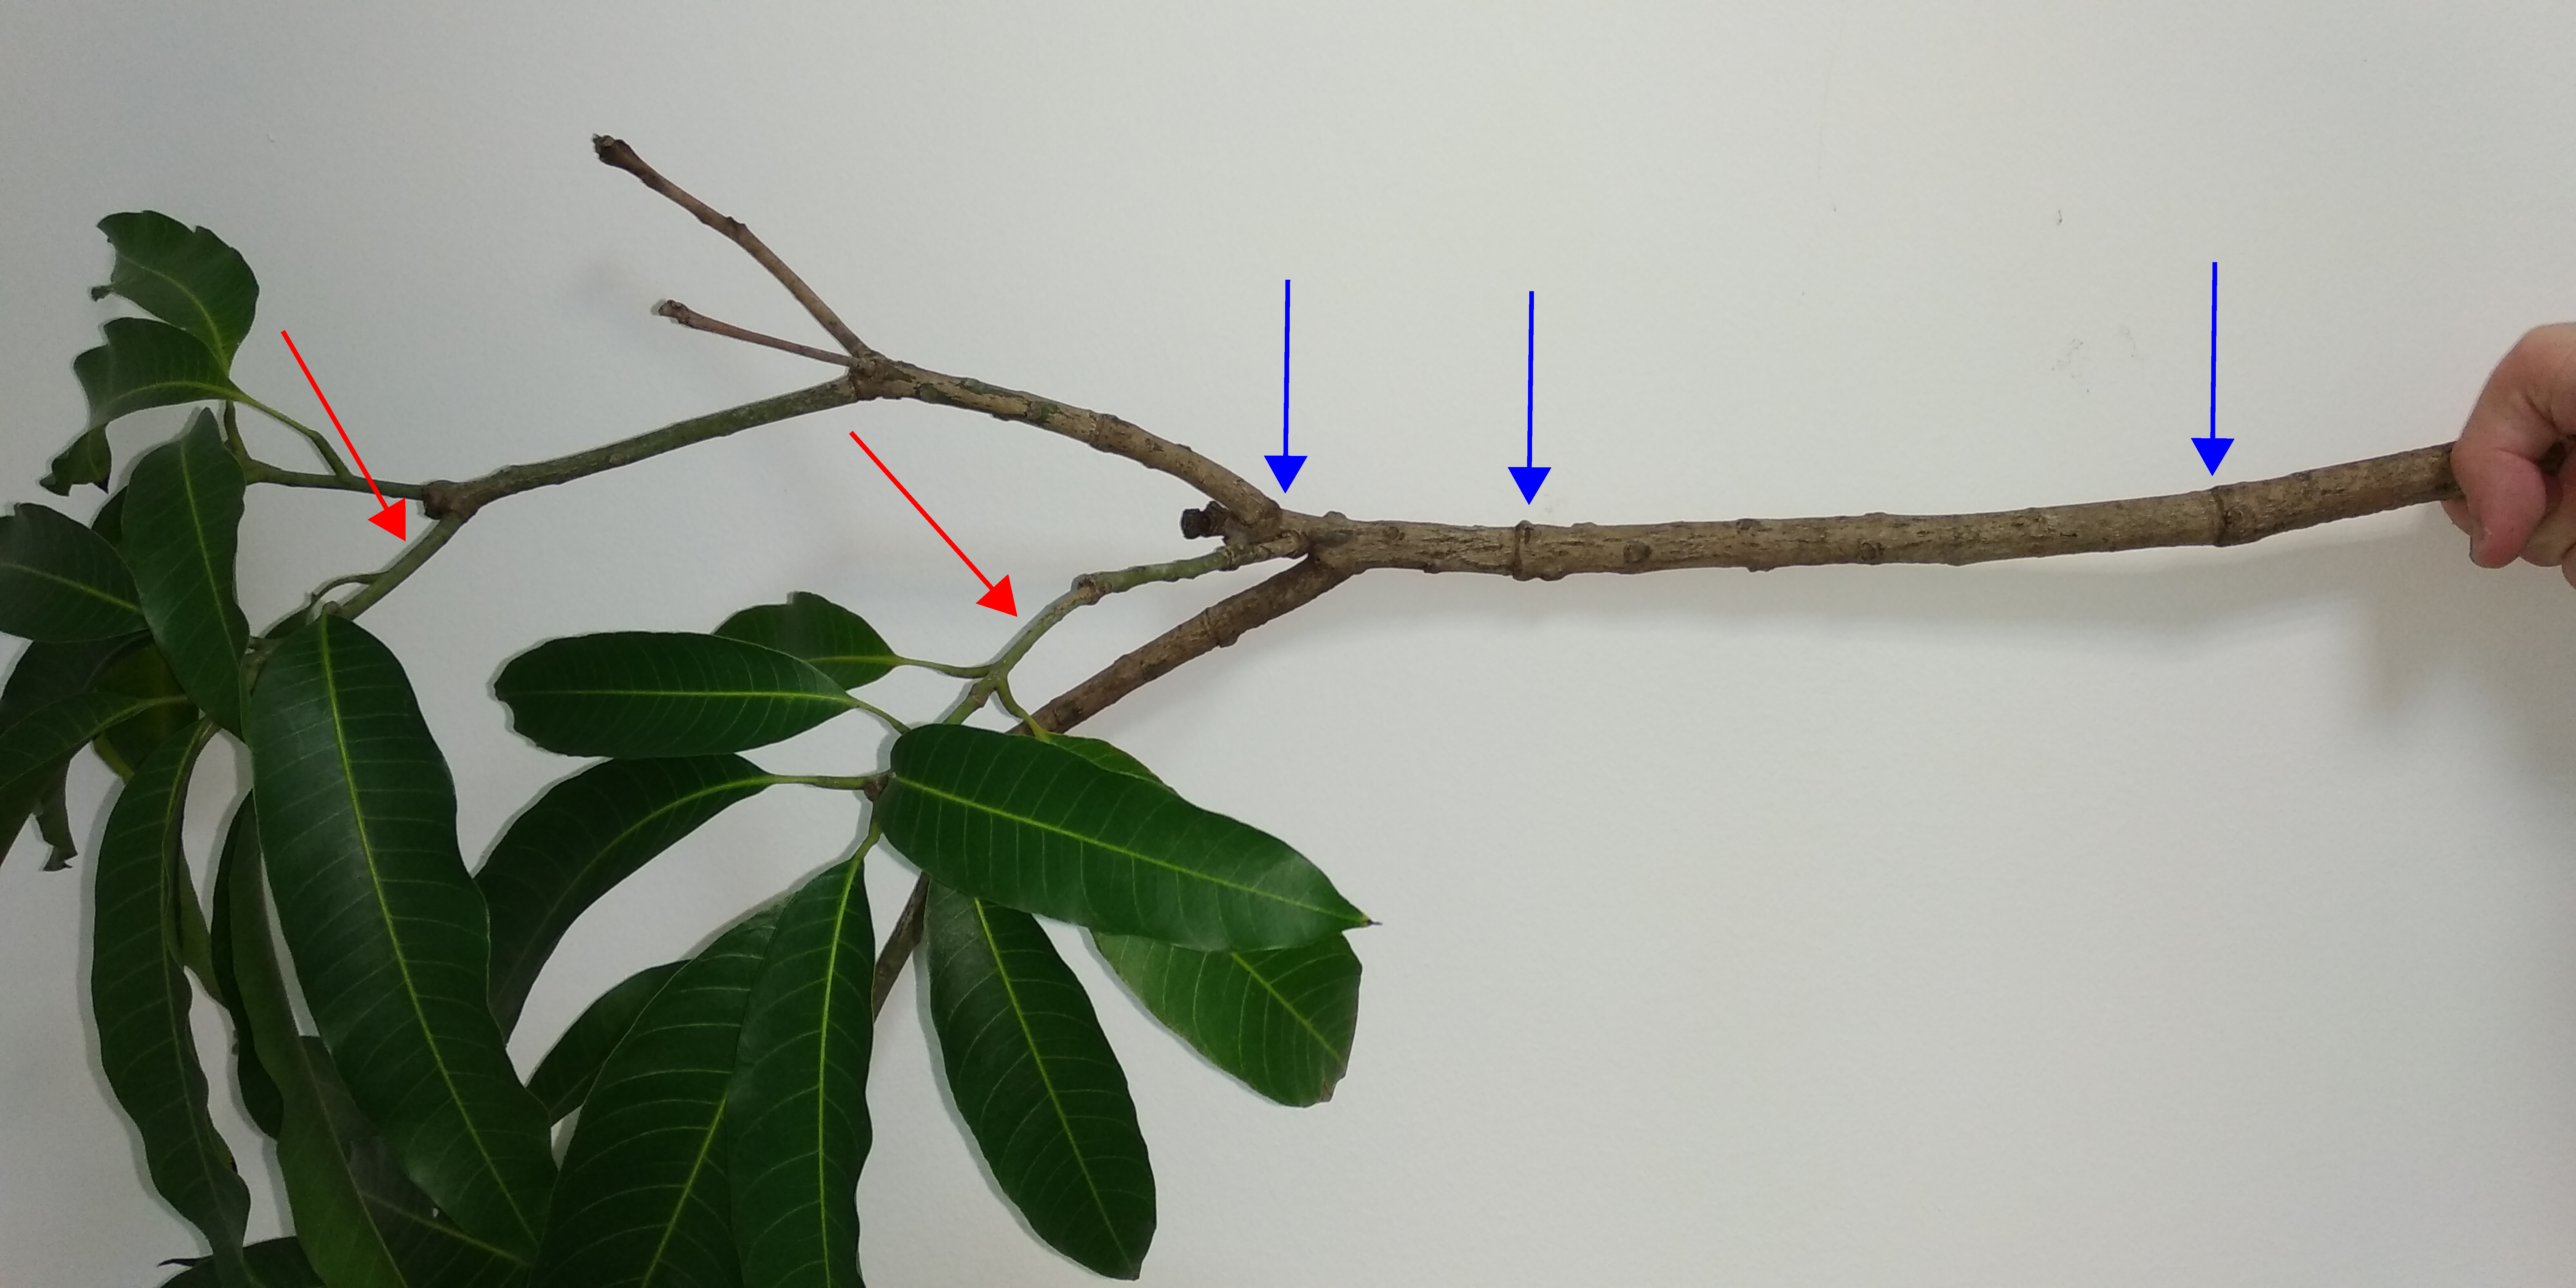
\includegraphics[scale = 0.1]{photos/branche.pdf}
 \caption{Photographie d'une branche portant des unités de croissance. Les flèches rouges montrent des unités de croissances. Les flèches bleues montrent les délimitations des unités de croissance antérieures ; la portion de la branche entre deux flèches bleues correspond à une ancienne unité de croissance qui a perdue ses feuilles, grossie et durcie et qui fait désormais partie intégrante de la branche.}
 \label{fig:uc}
\end{figure}


% \begin{wrapfigure}{r}{3.5in}
% %%%%%%%%%%%%%%%%%%%%%%%%%%%%%%%%%%%%%%%%%%%%%%%%%%%%%%%%%%%%%%%%%%%%%%%%%%%%%%%%%%%%%%%
% %%% You will need to add \usepackage{wrapfig} to your preamble to use textwrapping %%%
% %%%%%%%%%%%%%%%%%%%%%%%%%%%%%%%%%%%%%%%%%%%%%%%%%%%%%%%%%%%%%%%%%%%%%%%%%%%%%%%%%%%%%%%
%  \centering
%  \includegraphics[bb=0 0 3872 2592,scale=0.063]{photos/inflo.jpg}
%  % inflo.jpg: 3872x2592 px, 72dpi, 136.60x91.44 cm, bb=0 0 3872 2592
%  \caption{Une inflorescence (photo : F. Normand)}
%  \label{fig:inflo}
% \end{wrapfigure}
\newpage

Et ce sont ces unités de croissance qui portent les \emph{inflorescences}.
Les inflorescences désignent des groupements de bourgeons. De façon plus formelle, ce sont des «panicules pyramidales pouvant mesurer jusqu’à 30 cm».
Ces bourgeons se comptent par centaines voire milliers pour chaque inflorescence. 
Ils deviennent des fleurs mâles ou hermaphrodites.
Ces dernières deviennent des fruits, si elles sont fécondées.
En théorie.
En pratique, une très faible proportion donnera des fruits.
Même sans ravageurs et avec de bonnes conditions climatiques, il y a rarement plus de cinq fruits par inflorescences.
Par contre si les conditions sont défavorables, beaucoup d'inflorescences peuvent ne pas produire de fruit du tout.
Une photographie d'inflorescence est visible sur la figure~\ref{fig:inflo}.

\begin{figure}[ht]
 \centering
 \includegraphics[bb=0 0 3872 2592,scale=0.079]{photos/inflo.jpg}
 % inflo.jpg: 3872x2592 px, 72dpi, 136.60x91.44 cm, bb=0 0 3872 2592
 \caption{Une inflorescence (photo : F. Normand)}
 \label{fig:inflo}
\end{figure}




Du cycle phénologique viennent les \emph{stades phénologiques} des inflorescences.
Ils caractérisent le niveau de développement des inflorescences.
On considère ici les stades phénologiques allant de C à F.
Le stade C correspond au débourrement (l'éclosion des bourgeons) de l'inflorescence.
Le stade F s'étend entre l'apparition de la première fleur jusqu'à la disparition de la dernière.
Et les stades D et E représentent les étapes intermédiaires du développement qui mènent du débourrement à la floraison d'une inflorescence.
Les durées des stades phénologiques sont les suivantes :
\begin{center}
\begin{tabular}{llll}
Stade phénologique & C/D & E & F\\
Durée (en jours) & 7 & 9 & 34
\end{tabular}
\end{center}
Les inflorescences ont ainsi une durée de vie théorique de 50 jours \citep{laurie}.
Cette durée théorique peut être réduite en cas d'attaque de cécidomyies des fleurs, surtout lorsque l'inflorescence se fait attaquer lors des premiers stades, moment où elle est la plus vulnérable.

À la Réunion, les inflorescences commencent à apparaître en juillet, les premiers fruits apparaissent à la mi-septembre. 
La récolte a lieu de décembre à janvier.
Ces dates varient en fonction de la zone géographique.






\section{La cécidomyie des fleurs}
\label{chap:cecido}

Les cécidomyies des fleurs sont des diptères (des sortes de moucherons) dont le manguier est la seule plante-hôte.
À la Réunion, les cécidomyies sont présentes toute l'année et se reproduisent sur les inflorescences et les jeunes feuilles \citep{paul}.
Le nombre maximal est atteint pendant la période de floraison.

% \subsection{Cycle de développement}

Le cycle de développement de la cécidomyie des fleurs est schématisé sur la figure~\ref{fig:cycle}.
Les femelles présentes dans le verger au jour $t$ peuvent pondre jusqu'à 150 œufs dans les inflorescences.
Les œufs laissent place à des larves.
Au bout de sept à douze jours après la ponte, une fois le troisième stade de développement larvaire atteint, les larves s'éjectent des inflorescences en direction du sol.
(Et ce développement larvaire qui provoque des dégâts sur les inflorescences car les larves consomment le tissu végétal et creusent des galeries, fragilisant ainsi les inflorescences.)
Une fois au sol, les larves s'enfouissent dans le sol. 
Elles peuvent alors entrer en phase de \emph{pupaison}, qui correspond à la transformation de la larve en cécidomyie.
Cette phase dure quatre à six jours, et une fois finie les cécidomyies adultes émergent du sol et infestent le verger --- perpétuant ainsi le cycle. 
Une fois adultes, leur durée de vie n'excède pas 72 heures.

Alternativement à la pupaison, les larves peuvent aussi rentrer en \emph{diapause}.
La diapause peut être vue comme une sorte d'hibernation, où le cycle est mis en pause un an ou deux avant l'émergence de la cécidomyie adulte.


%
\begin{figure}
 \centering
 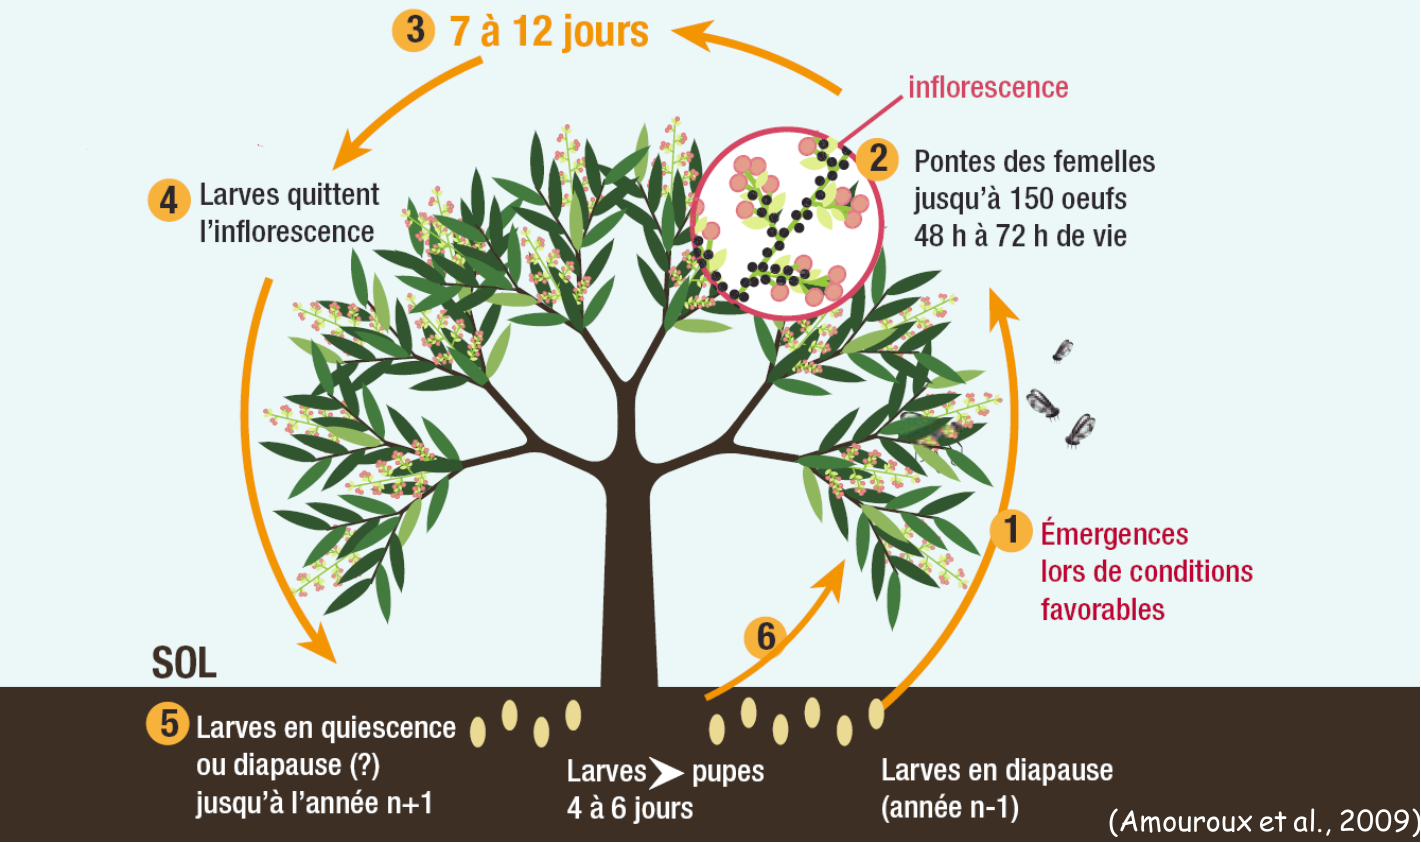
\includegraphics[scale = 0.33]{photos/cycle.png}
%  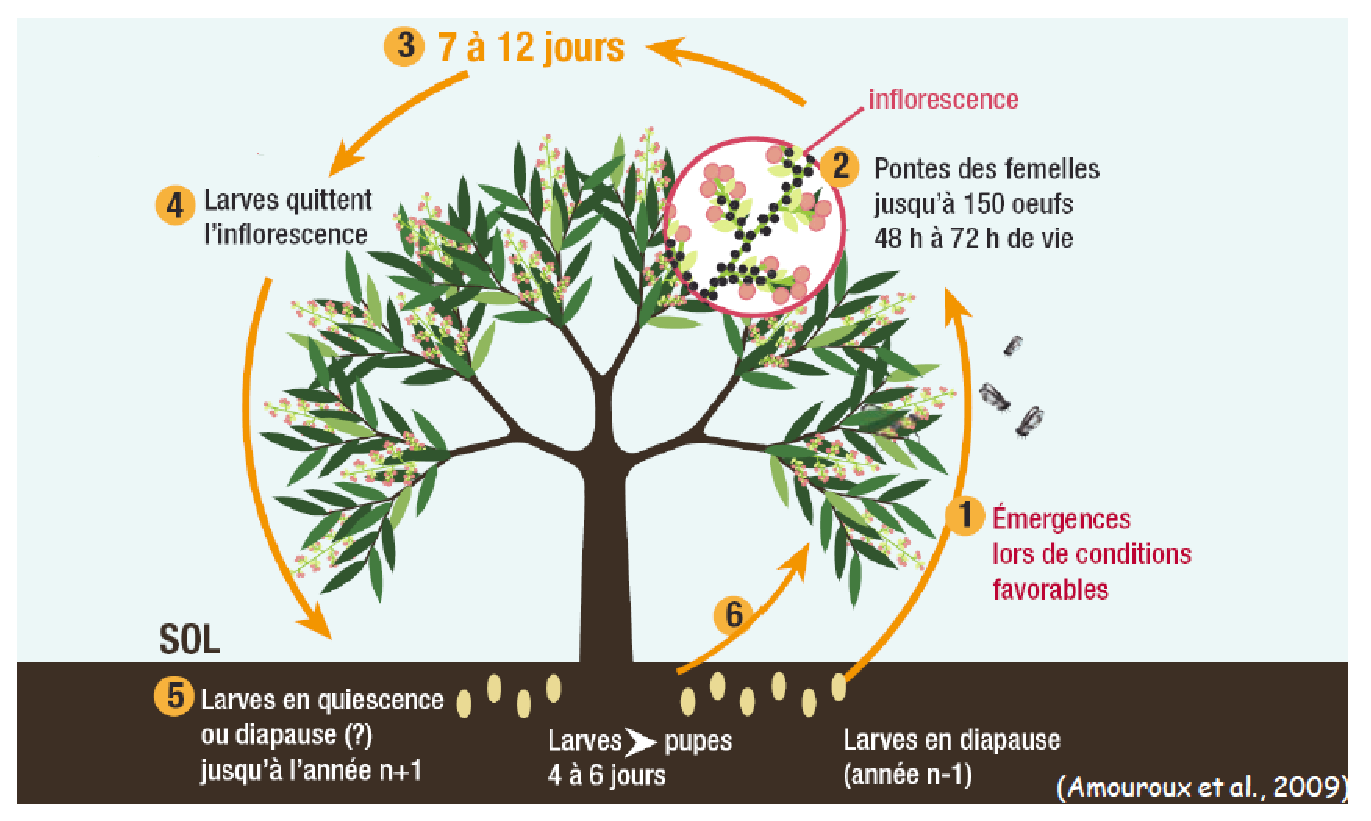
\epsfig{file = photos/cycle.eps, scale = 0.5}
 \caption{Représentation du cycle de développement de la cécidomyie des fleurs du manguier par \citet{paulguide}.}
 \label{fig:cycle}
\end{figure}
%

% \subsection{Titre random}

Les individus qui sortent de diapause permettent notamment le lancement de la dynamique d'infestation pendant la période de floraison.
La sortie est dû à une baisse de température qui coïncide avec le début de la floraison \citep{pauldiap}.


























% Chapitre 3
\chapter{Expérimentation réalisée et données disponibles} 

\lettrine{C}{e} chapitre explique l'expérimentation qui a été menée en 2017 sur deux vergers dans la commune de Saint-Paul (à la Réunion). 
On reviendra sur le dispositif de l'expérimentation et les données qui en ont étés tirées.
Le but de cette expérimentation était de déterminer quel est l'impact de la modalité de couverture du sol dans le degré d'infestation d'un verger.


\section{Dispositif}

Le verger expérimental (que l'on apellera aussi parcelle par la suite) n\textdegree1 a une superficie de 0.33 hectares et est séparé en trois sous-parcelles de tailles égales de trente arbres.
Sur chacune des trois sous-parcelle, une modalité de couverture du sol différente est mise en place.
Sur un côté il y avait un enherbement entretenu de sorte qu'il reste ras, la modalité \emph{enherbement ras (ER)} fera référence à ce traitement dans la suite du document.
La sous-parcelle du milieu fut baché, afin que les cécidomyies ne puissent ni entrer dans le sol ni en sortir ; cette modalité correspond au \emph{paillage synthétique (PS)}. 
La dernière partie fut laissée telle quelle, sans entretien particulier, donnant ainsi un \emph{enherbement haut (EH)}.
À noter qu'à côté de ce verger, il y en avait un autre.
Bien que cet autre verger n'avait aucun rôle particulier, il a probablement servi de source d'infestation exogène au verger expérimental.
Tout cela est schématisé sur la figure~\ref{fig:exp}.
Le dispositif sur la parcelle n\textdegree2 est décrit dans l'annexe~\ref{chap:bloc2}.
\begin{figure}[ht]
 \centering
 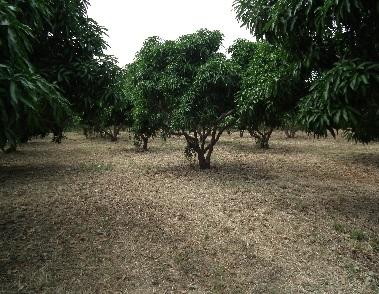
\includegraphics{photos/er.jpg}
 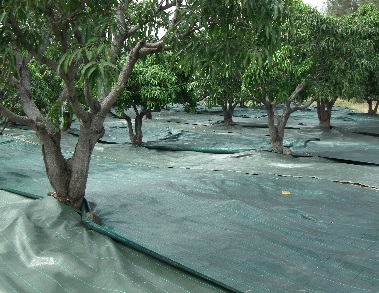
\includegraphics{photos/ps.jpg}
 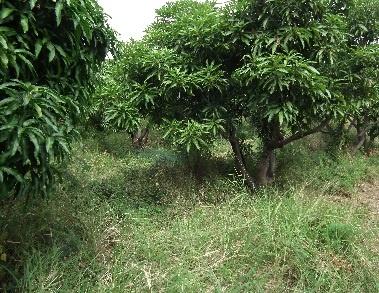
\includegraphics{photos/eh.jpg}
 
 \vspace*{0.5cm}
 
 \begin{tikzpicture}[scale = 0.4]
  \draw (0,5) rectangle (18, 12);
  \draw (6, 5) -- (6, 12);
  \draw (12, 5) -- (12, 12);
  \draw (-0.5, 0) -- (-0.5, 3) ;
  \draw (-0.5, 3) -- (18.5, 3) ;
  \draw (18.5, 3) -- (18.5, 0);
  \draw (9, 1.75) node{\text{ \footnotesize Autre verger de manguiers}};
  \draw (9, 0.75) node{\text{\footnotesize (possible source d'infestation)}};
  \draw (9, 9) node{\text{ \footnotesize Paillage}};
  \draw (9, 8) node{\text{ \footnotesize synthétique}};
  \draw (3, 9) node{\text{ \footnotesize Enherbement}};
  \draw (3, 8) node{\text{ \footnotesize ras}};
  \draw (15, 9) node{\text{ \footnotesize Enherbement}};
  \draw (15, 8) node{\text{ \footnotesize haut}};
  \draw (-0.5, 4.5) rectangle (18.5, 14);
  \draw (9, 13) node{\text{ \footnotesize Verger expérimental }};
 \end{tikzpicture}
 \caption{En haut, photographie des trois modalités : enherbement ras, paillage synthétique et enherbement haut.
 En bas, schéma de l'expérimentation menée.  Le verger sur lequel ont été testées les trois modalités de couvertures du sol était situé à côté d'un autre verger. Bien que cet autre verger n'avait pas de rôle particulier, il a probablement servi de source d'infestation exogène au verger expérimental.}
 \label{fig:exp}
\end{figure}

Sur ces deux vergers expérimentaux, deux types d'observations furent effectués entre juin et octobre 2017. 
Le premier porte sur les inflorescences. 
Huit unités de croissance furent sélectionnées sur chacun des vingt-cinq arbres échantillonés aléatoirement dans chacune des trois sous-parcelles.
Et c'est ainsi qu'entre le 26 juin et le 3 octobre 2017 furent notés les dates de débourrements des inflorescences présentes sur les deux cents unités de croissance suivies.
À partir du 6 septembre furent aussi notées les dates de morts des inflorescences. 
Les données de ce relevé seront rassemblées en un jeu de données que l'on nommera \emph{dataset 1}.

La seconde catégorie d'observations porte sur la capture des larves de cécidomyies.
Dans chacune des trois sous-parcelles, dix arbres furent sélectionnés. 
Sous chacun de ces arbres furent placés deux pièges en dessous des inflorescences présentes.
Les pièges sont des bidons plastiques carrés de douze centimètres de côté remplis d'eau.
À noter que les pièges furent déplacés au cours du temps pour qu'ils soient toujours en-dessous d'inflorescences.
Et c'est ainsi qu'entre le 18 juillet et le 6 octobre 2017 furent notés le nombre de larves piégées, le nombre d'inflorescences vivantes au-dessus du piège et le nombre d'inflorescences vivantes dans l'arbre.
Les données de ce relevé seront rassemblées en un jeu de données que l'on nommera \emph{dataset 2}.

\section{Données}

Après mise en forme des données\footnote{Tous les scripts utilisés sont disponibles à l'adresse \url{https://github.com/bastienreyne/cecidomyie}}, on peut extraire les dynamiques qui nous intéressent.
Il faut cependant noter que les deux jeux de données n'ont pas la même échelle.
On choisira de tout mettre à l'échelle de la sous-parcelle.

\subsection{Inflorescences vivantes}

On peut extraire les dynamiques d'inflorescences vivantes grâce aux deux jeux de données : elles seront notées $I^1_t$ pour le \emph{dataset 1} et $I^2_t$ pour le \emph{dataset 2}.
Pour le \emph{dataset 2}, c'est facile. 
On possède le nombre d'inflorescences vivantes dans les arbres suivis aux différentes dates; il suffit alors de mettre à l'échelle comme suit :
\[
I_{t}^{2} = \frac{N}{n}\sum_{k=1}^{n} I^{2}_{k, t},
\]
avec $N$ représentant le nombre d'arbre dans la sous-parcelle, $n$ le nombre d'arbre suivis et $I^{2}_{k, t}$ le nombre d'inflorescences sur l'arbre $k$ à la date $t$.
À noter que les relevés n'ont pas été effectués à chaque date $t$, le nombre d'inflorescences vivantes entre deux relevés effectif est alors le résultat d'une interpolation linéaire entre lesdits relevés.

Pour le \emph{dataset 1}, on possède le nombre de débourrements journalier $B_t$ et le nombre de morts journalier $D_t$.
Le nombre d'inflorescences vivantes au jour $t$ s'écrit alors
\[
I_t^1 = \alpha\left( \sum_{j=1}^{t} B_j - \sum_{j=1}^{t} D_j \right),
\]
où $\alpha$ représente le coefficient de mise à l'échelle pour passer de deux cents unités de croissance à la sous-parcelle.
Il faut cependant apporter une correction à cette dynamique.
En effet, l'observation des inflorescences mortes n'a été faite qu'à partir du 6 septembre.
De ce fait, sur ce jeu de données la distinction entre inflorescences vivantes et mortes n'est possible qu'à partir du 6 septembre.
Il en résulte une forte diminution du nombre d'inflorescences entre le 5 et le 6 septembre (voir figure~\ref{fig:inflos}).
Cet écart correspond au nombre de mort cumulé jusqu'au 6 septembre, et qu'il faut donc répartir sur la période concernée.
N'ayant aucune indication de comment la répartir, on utilisera la dynamique d'inflorescences vivantes du \emph{dataset 2} afin que la dynamique du \emph{dataset 1} y ressemble le plus possible --- et on en profitera au passage pour estimer le coefficient de mise à l'échelle $\alpha$.
Plus précisément, on attribuera un poids (à calibrer numériquement) pour tous les jours entre le jour 1 et le 5 septembre, et le nombre de morts chaque jour sera donné par la formule
\[
D_{t}^{c} = \frac{p_t\times m}{\sum_{j}p_j},
\]
où $D_{t}^{c}$ désigne le nombre de mort à la date $t$, $m$ le nombre de mort total déterminé par la différence d'inflorescences entre le 5 et 6 septembre et $p_t$ le poids assigné au jour $t$. 
Les poids $p_t$ et le coefficient de mise à l'échelle $\alpha$ seront déterminés numériquement afin de résoudre le problème
\[
\arg\max_{\alpha, p_t} \sum_{t}\left|I^{2}_{t} - I_{t}^{1, c}\right|, 
\]
où $I_{t}^{1, c}$ représente les inflorescences vivantes du \emph{dataset 1} mises à l'échelle et corrigées ; cette dynamique est determinée par la formule
\[
I_{t}^{1, c} = \begin{cases}
                I_t^1 - D_t^{c} & \text{si } t \leq 6 \text{ septembre},\\
                I_t^1 & \text{sinon}.
               \end{cases}
\]
Les différentes dynamiques d'inflorescences sont visibles sur la figure~\ref{fig:inflos}.
On remarque des dynamiques très différentes pour la modalité «enherbement haut», et ce même après correction de la dynamique issue du \emph{dataset 1}.
On peut expliquer ce phénomène par la grande variabilité de la phénologie chez le manguier ; ainsi des échantillonages différents peuvent produire des dynamiques très différentes.
Les deux autres modalités ont en revanche des dynamiques similaires (après correction).
\begin{figure}[ht]
\centering
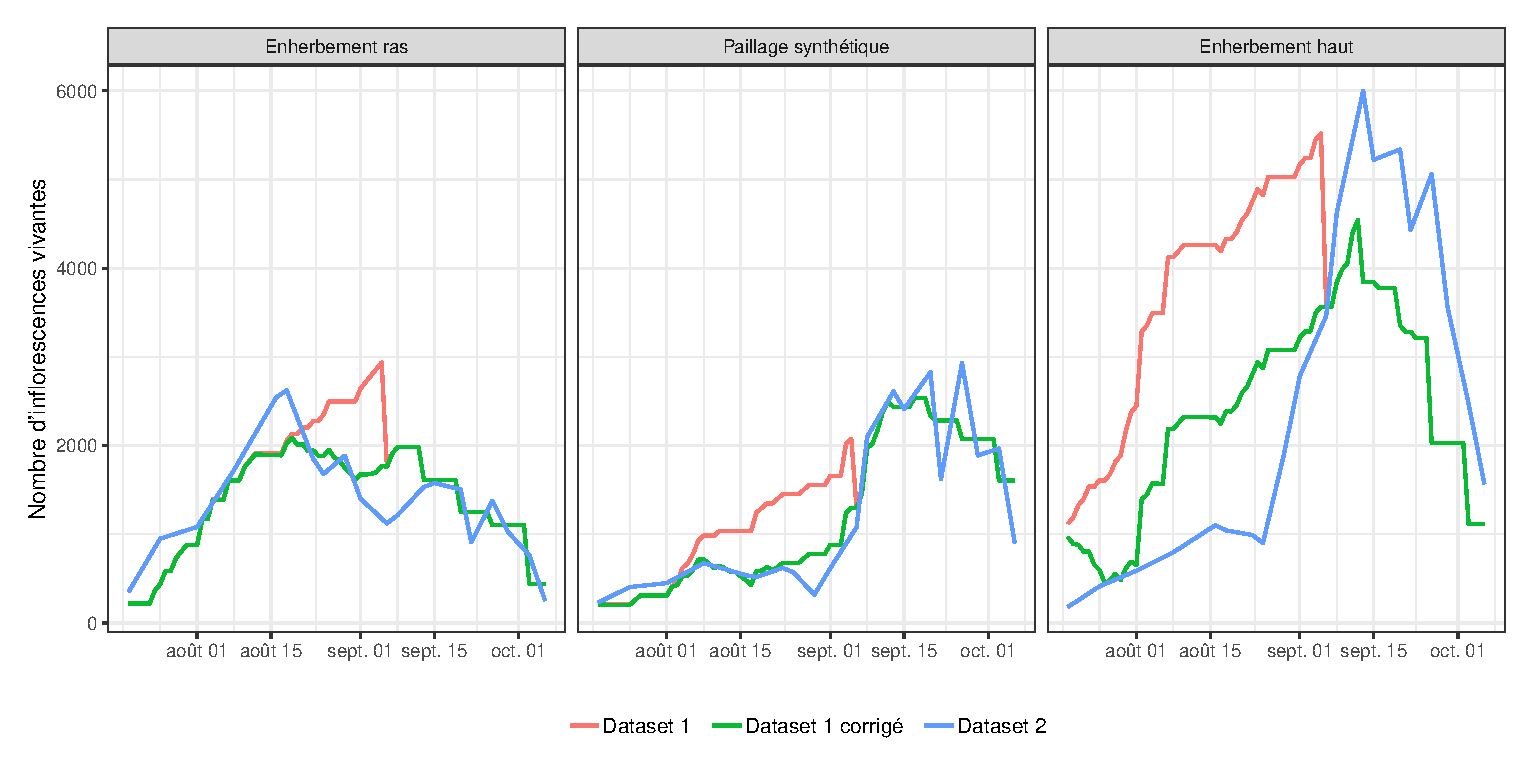
\epsfig{file = r/inflos_vivantes.eps, scale = 0.59}
\caption{Comparaison des différentes dynamiques d'inflorescences vivantes du verger n\textdegree1 en fonction du \emph{dataset} utilisé. Si après correction les dynamiques des deux \emph{datasets} sont similaires pour les deux premières modalités, la modalité «enherbement haut» présente des différences significatives entre les deux dynamiques. Cela peut s'expliquer par un échantillonage différent d'un phénomène présentant une grande variabilité.}
\label{fig:inflos}
\end{figure}

On fera le choix de privilégier, à chaque fois que cela s'avèrera possible, les dynamiques issues du \emph{dataset 2}.
Ce choix découle du fait que ce sont les dynamiques associées aux dynamiques de larves.


\subsection{Larves}

Le \emph{dataset 2} permet aussi de récupérer la dynamique de larves, à partir des larves piégées.
En effet, on connait le nombre de larves par piège, le nombre d'inflorescences vivantes situées au-dessus des pièges et le nombre d'inflorescences vivantes dans les arbres suivis.
De là, on peut estimer le nombre de larves qui s'éjecte des inflorescences à l'échelle d'un arbre, puis à l'échelle de la sous-parcelle.
Il y a cependant ici une subtilité : le relevé des pièges n'est pas quotidien, il faut donc répartir le nombre de larves piégées entre deux relevés effectifs sur la période entre lesdits relevés.
La dynamiques de larves peut donc s'obtenir en utilisant la formule 
\[
L_t = \frac{N}{n}\left(\sum_{k = 1}^n L_{t}^{k} \times \frac{I_{k, t}^{2}}{I_{k, t}^{2, p}} \right),
\]
où $N$ représente le nombre d'arbre dans la sous-parcelle, $n$ le nombre d'arbre suivis, $I^{2}_{k, t}$ le nombre d'inflorescences sur l'arbre $k$ à la date $t$, $I^{2, p}_{k, t}$ le nombre d'inflorescences au-dessus des pièges dans l'arbre $k$ à la date $t$ et on définit $L_t^k$ par
\[
L_t^k = \frac{L_{k, t}^j}{t^j - t^{j-1}},
\]
avec $t_j$  le nombre de jours entre la première observation et le $j^{\text{ème}}$ relevé et $L_{k, t}^j$ le nombre de larves dans les pièges de l'arbre $k$ au $j^{\text{ème}}$ relevé.
Les différentes dynamiques de larves sont visibles sur la figure~\ref{fig:larves}.
\begin{figure}[ht]
\centering
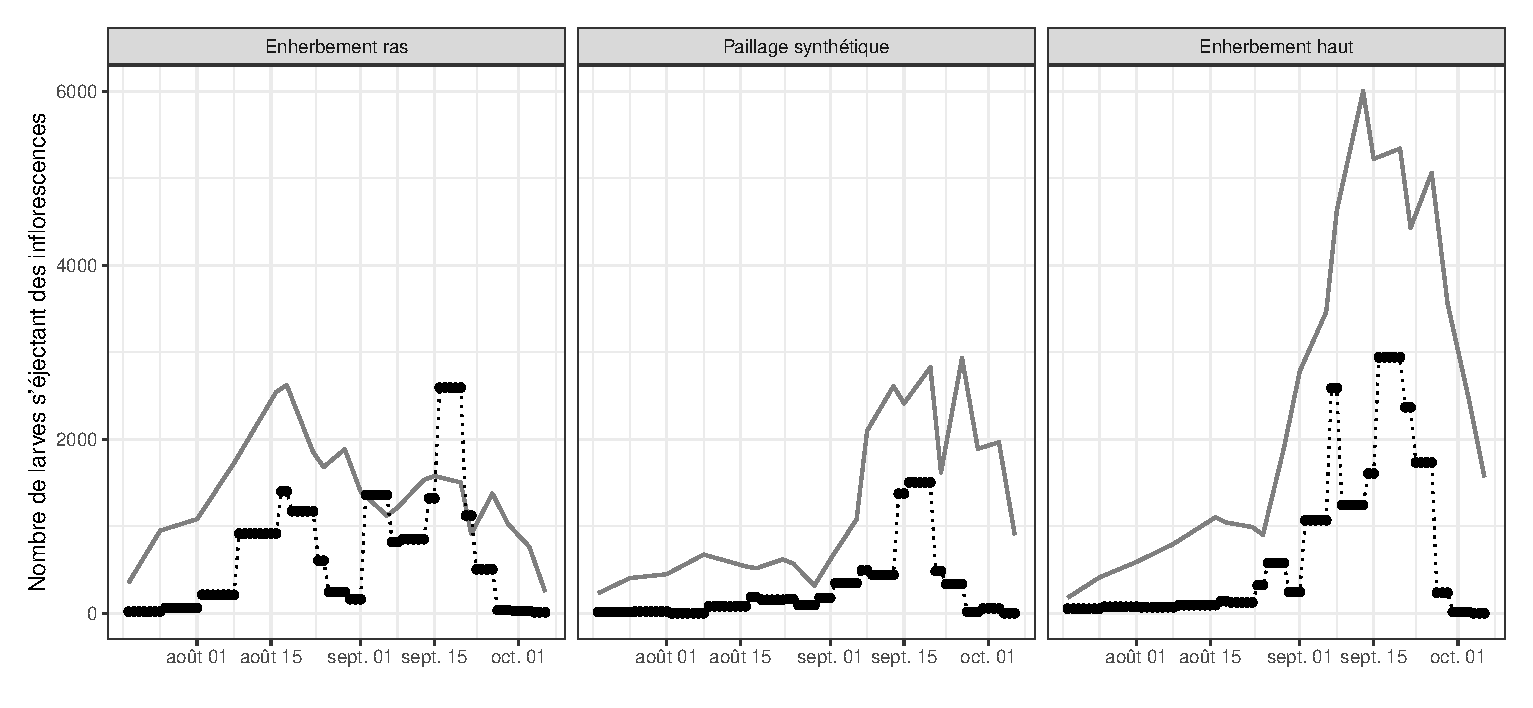
\epsfig{file = r/larves.eps, scale = 0.59}
\caption{Dynamiques de larves s'éjectant des inflorescences des manguiers chaque jour dans le verger n\textdegree1 pour chacune des trois sous-parcelles. En gris sont visibles les dynamiques d'inflorescences vivantes (issues du \emph{dataset 2}, $I^2_t$).}
\label{fig:larves}
\end{figure}

Les dynamiques pour le verger n\textdegree2 sont visibles dans l'annexe~\ref{chap:bloc2}.


% Chapitre 4
\chapter{Le modèle}

\lettrine{O}{n} s'intéresse ici aux différentes approches possibles pour modéliser le système manguier~--~cécidomyies des fleurs. 
Il y a dans la littérature quelques modèles relatifs aux manguiers et aux cécidomyies.
% On décrira la solution retenue ainsi que les hypothèses faites.

Concernant la modélisation en rapport avec le manguier, on peut citer le modèle \emph{Virtual Mango} développé par \citet{fred}.
C'est un modèle qui simule le développement architectural du manguier, ainsi que la croissance et les différents stades phénologiques des unités de croissance et des inflorescences et la croissance des fruits.
Le modèle ne prend cependant pas en compte l'impact des ravageurs sur le développement de l'arbre et sa production.

Concernant la modélisation en rapport avec les cécidomyies des fleurs, on peut noter l'existence d'un modèle de colonisation d'un verger par les cécidomyies \citep{paul}. 
Les données utilisées proviennent d'une expérimentation menée sur un verger entièrement bâché. 
C'est un modèle stochastique et spatialisé qui prend en compte l'arrivée des femelles sur le verger, leurs pontes d'œufs dans les inflorescences, le développement de ces derniers jusqu'au troisième stade de développement larvaire et enfin l'éjection des larves des inflorescences.
Cependant, le fait que le verger modélisé est entièrement bâché implique l'abscence de cycle de développement complet pour les cécidomyies à l'intérieur du verger ainsi que l'absence d'émergence de cécidomyies issues de la diapause.

On choisira ici l'approche amorcée par \citet{laurie}, qui propose une modélisation non spatialisée du verger expérimental considérant l'infestation du verger par des femelles exogènes et la reproduction endogène, tout en prenant en compte les différentes modalités de couverture du sol.
L'objectif sera de simuler les dynamiques de larves à l'échelle de la sous-parcelle en fonction du nombre d'inflorescences présentes.

\section{Approche retenue et hypothèses}

L'approche retenue se veut simple.
On considèrera les populations (de cécidomyies et d'inflorescences vivantes) dans chaque sous-parcelle et non les individus.
Concrètement, cela veut dire que l'on ne considèrera que les nombres totaux d'inflorescences vivantes et de cécidomyies qu'il y a chaque jour dans chaque sous-parcelle.
Par ailleurs, la période considérée est la saison de floraison et le modèle n'est pas pluriannuel.

Les hypothèses sur les processus biologiques qui régissent le système, que nous faisons, sont :
\begin{itemize}
 \item la modalité de couverture du sol n'influe pas sur le développement et la phénologie du manguier, elle n'influe pas non plus sur le déplacement des cécidomyies ;
 \item la durée de vie des femelles n'est que d'un jour, et il correspond au jour de la ponte ;
 \item aucune cécidomyie (larve ou adulte) ne rentre dans le sol ou ne sort du sol pour la sous-parcelle avec un paillage synthétique ;
 \item il y a un taux de mortalité pour larves lorsqu'elle rentrent ou et les adultes lorsqu'ils sortent du sol, et ce taux est différent entre l'enherbement ras et l'enherbement haut ;
 \item les larves qui n'entrent pas en pupaison (soit qui meurent, soit qui rentrent en diapause) sont exclues du système ;
 \item la probabilité d'entrer en pupaison dépend de la température ;
 \item la quantité de cécidomyies en diapause est la même pour les trois sous-parcelles;
 \item un individu qui émerge dans une sous-parcelle peut se déplacer dans les autres sous-parcelles, il y a cependant un coût relatif à la distance (autrement dit, les cécidomyies préfèrent rester dans la sous-parcelle dans laquelle elles émergent, puis aller dans la sous-parcelle limitrophe plutôt que dans la troisième) ;
 \item les femelles exogènes arrivent proportionnellement aux inflorescences vivantes dans la parcelles (qui exercent un effet d'attraction) ;
 \item s’il y a significativement plus de femelles que d’inflorescences, alors elles ne peuvent pas toutes pondre ;  
 \item il y a un taux de mortalité sur les œufs pondus par les femelles, ils ne donneront pas tous des larves.
%  \item  seuls les premiers stades phénologiques de l'inflorescence sont attractifs pour les cécidomyies.
\end{itemize}

On reprend le cycle de développement de la cécidomyie présenté dans la partie~\ref{chap:cecido}, et on essaye de le traduire par des équations simples.

\section{Formalisme}

Le schéma conceptuel du modèle est visible sur la figure~\ref{fig:schema}. On le détaille ci-dessous.

Le nombre de larves est donné par 
\[
 L_{t, i} = F_{t - d_{\ell}, i} \times R \times E_0 \times \mu_{\ell}.
\]
Ici, $L_{t,i}$ désigne le nombre de larves qui s'éjectent des inflorescences à la date $t$ dans la sous-parcelle $i$, $F_{t - d_{\ell}, i}$ le nombre de femelles qu'il y avait dans la sous-parcelle $i$ une durée de développement larvaire auparavant (durée qu'il y a entre la ponte des œufs et l'apparition du dernier stade larvaire où les larves s'éjectent des inflorescences pour s'enfouir dans le sol), $R$ représente la disponibilité d'inflorescences pour les cécidomyies, $E_0$ le nombre maximal d'œufs pondus par une femelle et $\mu_{\ell}$ la probabilité de survie des œufs et larves.
En d'autres termes, cela signifie simplement que le nombre de larves à une certaine date résulte du nombre d'œufs pondus par les femelles, qui ont survécus et se sont développés --- sans oublier de prendre en compte que le développement dure quelques jours et que le nombre de femelles qui pond est conditionné à la disponibilité en ressources.

% La deuxième équation donne le nombre de femelles issues du cycle de pupaison qui émergent dans le verger :
% \begin{equation}
% F^{\text{pupe}}_{t, i} = L_{t - d_{\text{p}}, i} \times \mu_{\text{sol}} \times p_{\text{p}} \times \frac{1}{1 + \mathit{SR}}.
% \label{eq:fpupe}
% \end{equation}
% On a ici $F^{\text{pupe}}_{t}$ qui désigne le nombre de femelles issues du cycle de pupaison qui émergent à la date $t$ dans le verger, $L_{t - d_{\text{p}}}$ le nombre de larves qui sont rentrés dans le sol une durée de pupaison auparavant, $\mu_{\text{sol}}$ la probabilité pour une larve d'entrer dans le sol (qui dépend de la modalité de couverture du sol), $p_{\text{p}}$ la probabilité pour une larve d'entrer en phase de pupaison et d'y survivre et $\frac{1}{1 + \mathit{SR}}$ la proportion de larves qui se transforment en femelles (les mâles ne pondant pas, ils ne nous intéressent pas).
% Cela signifie les femelles issues de la phase de pupaison qui émergent à une certaine date correspond au nombre de larves qui ont réussies à pénétrer dans le sol, qui sont entrées en pupaison, se sont transformées en cécidomyies, ont survécues puis ont émergées --- en prenant en compte la durée de développement et la proportion de femelles chez les cécidomyies.


Dans l'équation ci-dessus, le coefficient $R$ est donné par
\[
R = \min\!\left\{1, \frac{k I_{t, i}}{ F_{t, i}} \right\}\!.
\]
Ce coefficient traduit la disponibilité en ressources pour les cécidomyies, c'est-à-dire que lorsqu'il n'y a pas suffisament d'inflorescences dans le verger par rapport au nombre de femelles, alors toutes les femelles ne peuvent pas pondre.
Il vaut 1 lorsque toutes les cécidomyies femelles peuvent pondrent ; il est compris entre 0 et 1 lorsque certaines cécidomyies femelles ne peuvent pas pondre.
Ce coefficient $R$ dépend du paramètre $k$ qui indique combien de femelles peut acceuillir une inflorescence chaque jour.

Toujours dans l'équation donnant le nombre de larves, on peut noter que le nombre de femelles présente dans la sous-parcelle $i$ au jour $t$ est donné par
\[
F_{t, i} = F^{\text{endo}}_{t, i\rightarrow i} + F^{\text{endo}}_{t, (j,k)\rightarrow i} + F^{\text{exo}}_{t, i}\!,
\]
où $F^{\text{endo}}_{t, i\rightarrow i}$ sont les femelles qui émergent dans la sous-parcelle $i$ et qui y restent, $F^{\text{endo}}_{t, (j,k)\rightarrow i}$ sont les femelles qui ont émergées dans les sous-parcelles $j$ et $k$ et qui viennent dans la sous-parcelle $i$, $F^{\text{exo}}_{t, i}$ sont les femelles exogènes à la parcelle qui viennent dans la sous-parcelle $i$.
Et le nombre de femelles exogènes est déterminé par
\[
F^{\text{exo}}_{t, i} = \gamma \times I_{t, i},
\]
avec $\gamma$ à déterminer.
Il y a aussi des échanges, entre les différentes sous-parcelles, de femelles qui ont émergées dans la parcelle.
Ainsi, le nombre de femelles qui ont émergées dans la sous-parcelle $i$ et qui vont dans la sous-parcelle $j$ est donné par
\[
F_{t, i \rightarrow j}^{\text{endo}} = \frac{I_{t, j} \times p_{\text{m}}^{\delta(i, j)}}{\sum_{n\in \{i,j,k\}} I_{t, n} \times p_{\text{m}}^{\delta(i, n)}},
\]
où $p_{\text{m}} \in [0; 1]$ et $\delta(i, n) =
\begin{cases}
0 & \text{ si } i=n \text{ (même sous-parcelle),}\\
1 & \text{ si $i$ et $n$ sont des sous-parcelles limitrophes,}\\
2 & \text{ si $i$ et $n$ sous-parcelles non-limitrophes.}\\
\end{cases}$\\
Le paramètre $p_{\text{m}}$ traduit l'intensité de la migration et le paramètre $\delta$ traduit «l'effet distance» (autrement dit, les cécidomyies préfèrent se déplacer le moins possible).

On peut noter que les femelles qui émergent comprennent les femelles issues de la phase de pupaison et celles issues de la sortie de diapause. Ainsi, on a
\[
F^{\text{endo}}_{t, i} = F^{\text{pupe}}_{t, i} + F^{\text{diap}}_{t,i},
\]
avec
\[
F^{\text{pupe}}_{t, i} = L_{t - d_{\text{p}}, i} \times \mu_{\text{sol}} \times p_{\text{p}} \times \frac{1}{1 + \mathit{SR}}.
\]
On a ici $F^{\text{pupe}}_{t, i}$ qui désigne le nombre de femelles issues du cycle de développement et qui émergent des pupes présentent dans le sol de la sous-parcelle $i$ à la date $t$, $L_{t - d_{\text{p}}, i}$ le nombre de larves qui sont rentrés dans le sol de la sous-parcelle $i$ une durée de pupaison auparavant, $\mu_{\text{sol}}$ la probabilité pour une larve d'entrer dans le sol (qui dépend de la modalité de couverture du sol), $p_{\text{p}}$ la probabilité pour une larve d'entrer en phase de pupaison et d'y survivre et $\mathit{SR}$ le ratio du nombre de mâles sur le nombre de femelles. 
Ainsi, $\frac{1}{1 + \mathit{SR}}$ donne la proportion de larves qui se transforment en femelles (les mâles ne pondant pas, ils ne nous intéressent pas).
Cela signifie les femelles issues de la phase de pupaison qui émergent à une certaine date correspond au nombre de larves qui ont réussies à pénétrer dans le sol, qui sont entrées en pupaison, se sont transformées en cécidomyies, ont survécues puis ont émergées --- en prenant en compte la durée de développement et la proportion de femelles chez les cécidomyies.
Il faut cependant noter que l'on a
\[
\mu_{\text{sol}} = \mu_{\text{sol}}^1 \times \mu_{\text{sol}}^2,
\]
où $\mu_{\text{sol}}^1$ correspond à la probabilité de survie d'une larve à la modalité de couverture du sol lorsqu'elle s'enfouit dans le sol et $\mu_{\text{sol}}^2$ désigne la probabilité de survie à la modalité de couverture du sol d'une femelle qui émerge du sol.
Cette distinction est nécessaire car les femelles qui sortent de diapause ne sont impactées par la modalité de couverture du sol qu'à la sortie des femelles (les larves étant entrées dans le sol avant la mise en place du dispositif).
On posera néanmoins, par souci de simplicité, $\mu_{\text{sol}}^1 = \mu_{\text{sol}}^2$.
Le nombre de femelles qui sortent de diapause est donné par 
\[
F_{t, i}^{\text{diap}} = D_{t} \times \frac{1}{1 + \mathit{SR}} \times \mu^{2}_{\text{sol}},
\]
où $D_{t}$ est le nombre de larves en diapause des années précédentes qui sort au jour $t$.
Le stock total de larves en diapause est donné par
\[
\texttt{stock} = \sum_t D_t.
\]


%% SCHÉMA
\begin{figure}[ht]
 \centering
 \begin{tikzpicture}[scale = 0.9]
 \draw (0, 0) node{\small \textsc{sol}};
  \draw [line width = 1.5mm, color = gray] (0.5, 0) -- (15, 0);
  % RECTANGLES
  \draw (0.7,  -1.5) rectangle (2.4,  -2.5); %diap + mort
%   \draw (8.4,  -1.5) rectangle (10.1, -2.5); % P
  \draw (12.5, -1.5) rectangle (14.2, -2.5); %Diap
  \draw (4.3,   1.5) rectangle (6,   2.5); % L
  \draw (9.4,   1.5) rectangle (11.1,  2.5); % N pupe
  \draw (11.5,  1.5) rectangle (13.2,  2.5); % N diap
  \draw (9.1,   1.2) rectangle (13.5,  3.4); % N emer
  \draw (4.3,   7) rectangle (6,   8); % N exo
  \draw (0.7,   4.5) rectangle (2.4,   5.5); % N voisins
  \draw (8.4,   4.5) rectangle (10.1,  5.5); % N endo
  \draw (12.5,  4.5) rectangle (14.2,  5.5); % N degage
  \draw (4.3,   4.5) rectangle (6, 5.5); % N
  % TEXTES CASES
  \draw (1.55, -2) node {\small Exclus};
  \draw (1.55,  5) node {\small $F^\text{endo}_{(j,k) \rightarrow i}$};
  \draw (5.15,   7.5) node {\small $F^\text{exo}_{i}$};
  \draw (5.15,   2) node {\small $L_{i}$};
  \draw (5.15,   5) node {\small $F_{i}$};
  \draw (13.35, 5) node {\small $F^\text{endo}_{i\rightarrow (j,k)}$};
  \draw (9.25,  5) node {\small $F^\text{endo}_{i\rightarrow i}$};
%   \draw (9.25, -2) node {\small $P_{i}$};
  \draw (13.35,-2) node {\small $D_{i}$};
  \draw (12.35, 2) node {\small $F^{\text{diap}}_{i}$};
  \draw (10.25, 2) node {\small $F^{\text{pupe}}_{i}$};
  \draw (11.3,  3) node {\small $F^{\text{endo}}_{i}$};
  \draw (0.8, 5.7) node {\small $\textcolor{blue}{t}$};
  \draw (4.4, 5.7) node {\small $\textcolor{blue}{t}$};
  \draw (4.4, 8.2) node {\small $\textcolor{blue}{t}$};
  \draw (4.8, 2.7) node {\small $\textcolor{blue}{t + d_{\ell}}$};
%   \draw (8.85, -1.3) node {\small $\textcolor{blue}{t + d_{\ell}}$};
  \draw (13, -1.3) node {\small $\textcolor{blue}{t + d_{\ell}}$};
  \draw (10, 3.65) node {\small $\textcolor{blue}{t + d_{\ell} + d_{\text{p}}}$};
  \draw (9.3, 5.75) node {\small $\textcolor{blue}{t + d_{\ell} + d_{\text{p}}}$};
  \draw (13.4, 5.75) node {\small $\textcolor{blue}{t + d_{\ell} + d_{\text{p}}}$};
  % LIGNES FLECHES
  \draw [line width=0.9]     (5.1,   1.5) -- (5.1,  -2);
  \draw [->,  line width=0.9] (5.1,  -2  ) -- (2.4,  -2);
%   \draw [->,  line width=0.9] (5.1,  -2  ) -- (8.4,  -2);
\draw [line width=0.9] (5.1,  -2  ) -- (10.8,  -2);
  \draw [line width=0.9]     (10.1, -2  ) -- (10.8, -2);
  \draw [line width=0.9]     (12.5, -2  ) -- (11.8, -2);
  \draw [->,  line width=0.9] (10.8,  -2 ) -- (10.8,  1.5);
  \draw [->,  line width=0.9] (11.8,  -2 ) -- (11.8,  1.5);
  \draw [line width=0.9]     (11.3,  3.4) -- (11.3,  5);
  \draw [->,  line width=0.9] (11.3,   5 ) -- (10.1,  5);
  \draw [->,  line width=0.9] (11.3,   5 ) -- (12.5,  5);
  \draw [->,  line width=0.9] (14.2,   5 ) -- (14.8,  5);
  \draw [->,  line width=0.9, dashed] (8.4,   5) -- (6, 5);
  \draw [->,  line width=0.9] (5.5,  4.5) -- (5.5, 2.5);
  \draw [->,  line width=0.9] (5.15,   7 ) -- (5.15,  5.5);
  \draw [->,  line width=0.9] (2.4,   5 ) -- (4.3,  5);
  % PARAMÈTRES
  \draw (5.6, 0.4)   node {\small $\mu_{\text{sol}}^1$};
  \draw (11.32, 0.4) node {\small $\mu_{\text{sol}}^2$};
%   \draw (6.8, -2.3)    node {\small $p_{\text{p}}$};
\draw (7.9, -2.3)    node {\small $p_{\text{p}}$};
  \draw (3.8, -2.3)    node {\small $1-p_{\text{p}}$};
  \draw (11.32, -0.42)  node {\small $\frac{1}{1 + \mathit{SR}}$};
  \draw (5.75, 4.1)     node {\small $R$};
  \draw (5.8, 3.5)     node {\small $E_0$};
  \draw (5.8, 2.9)     node {\small $\mu_\ell$};
 \end{tikzpicture}
 \caption{Schéma conceptuel du modèle pour la sous-parcelle $i$. En bleu est visible la date, la flèche en pointillés marque une rupture du temps.}
 \label{fig:schema}
\end{figure}


Le tableau~\ref{tab:param} recense les paramètres du modèle.


    \clearpage% Flush earlier floats (otherwise order might not be correct)

    \begin{landscape}% Landscape page
\begin{table}
\caption{Les différents paramètres du modèle.}
\label{tab:param}
\centering
{
\begin{tabular}{p{2cm}p{11.9cm}p{5cm}}
\textbf{Paramètre} & \textbf{Définition} & \textbf{Valeur}\\
$\gamma$ & Paramètre régulant l'arrivée des individus exogènes au verger & Calibration\\
$p_{\text{m}}$ & Paramètre régulant l'intensité des échanges entre sous-parcelles & Calibration\\
$\mu_{\text{sol}}^1$ & Probabilité de survie des larves lorsqu'elles s'enfouissent dans le sol à la modalité de couverture du sol & Calibration\\
$\mu_{\text{sol}}^2$ & Probabilité de survie des femelles qui émergent (de pupaison ou de diapause) la modalité de couverture du sol & Calibration\\
$k$ & Paramètre quantifiant le nombre de femelles que peut acceuillir une inflorescence chaque jour & Calibration\\
\texttt{stock} & Nombre d'individus entrés en diapause les années précédentes qui émergent l'année considérée & Calibration  \\
$E_0$ & Nombre maximal d'œufs pondus par une femelle & $\sim\!150$ \citep{paul}\\
$\mu_{\ell}$ & Probabilité de survie des œufs et des larves & $\sim\!0.04$ \citep{paul}\\
$\mathit{SR}$ & \textit{Sex-ratio} & 0.5 \citep{paul}\\
$p_{\text{p}}$ & Probabilité pour une larve d'entrer en phase de pupaison et d'y survivre & $\sim\! 0.77$ \citep{pauldiap}\\
$d_{\ell}$ & Durée (en jours) de la période entre la ponte et l'appartition du troisième stade de développement larvaire & 7 à 12 \citep{paul} \\
$d_{\text{p}}$ & Durée (en jours) de la phase de pupaison & 4 à 6 \citep{paul}
\end{tabular}
}
\end{table}
    \end{landscape}

% 
% \clearpage
% 
% \section{Inflorescences}
% 
% Le modèle prendra en entrée les inflorescences.
% Il faut cependant noter qu'il ne prendra pas les inflorescences «brutes», mais des dynamiques modifiées.
% En effet, on émet également l'hypothèse que les cécidomyies n'attaquent non pas les toutes les inflorescences mais uniquement celles se situant au stades phénologiques C, D ou E.
% Ce qui correspond aux seize premiers jours de l'inflorescence.
% Pour parvenir à avoir lesdites dynamiques, on a besoin de procéder à quelques étapes intermédiaires.
% On a notamment besoin de la date de débourrements des inflorescences avant d'avoir une estimation des dynamiques voulues.
% 
% \subsection{Débourrements}
% 
%  Afin de pouvoir simuler des dynamiques d'inflorescences avec une durée de vie de seize jours, il est nécessaire d'avoir les dates de débourrements des inflorescences.
%  Dans le verger n\textdegree1, les dynamiques pour les modalités «enherbement ras» et «paillage synthétique» issues des deux jeux de données ont des dynamiques plutôt similaires ; on pourrait donc utiliser les débourrements du \emph{dataset 1} mis à l'échelle.
%  En revanche, pour la modalité «enherbement haut», on observe des dynamiques très différentes. 
%  Et comme l'on souhaite privilégier les dynamiques issues du \emph{dataset 2}, il faut procéder autrement.
%  (Il en va de même pour les modalités «enherbement ras» et «paillage synthétique» du verger n\textdegree2.)
%  
%  L'objectif est alors de simuler les dates de débourrements qui permettent de produire la dynamique d'inflorescences vivantes du \emph{dataset 2}.
%  Pour cela, on suppose que la durée de vie effective d'une inflorescence suit une loi normale.
%  On possède les durées de vies effectives dans le \emph{dataset 1}.
%  Premièrement, en fixant le risque de première espèce à $\alpha = 5\%$, un test de normalité de Shapiro--Wilk nous confirme la normalité ($p$-valeur de 0.05447, on ne rejette donc pas l'hypothèse de normalité).
%  Deuxièmement, on observe une durée de vie effective moyenne de 29 jours (avec un écart-type de 14).
%  Ainsi, il faut donc simuler des débourrements, pour que des inflorescences ayant une durée de vie qui suit une $\mathcal{N}\left( 29; 14 \right)$, donne la dynamique d'inflorescences vivantes du \emph{dataset 2}.
%  Il faut donc trouver les $B_t$ tels que 
%  \[
%  I_{t}^{2} = B_t + \sum_{j = 1}^{50} B_{t - j} \times \left( 1 - F\left( j \right) \right),  \qquad \text{ avec } B_{t} = 0 \text{ si } t \leq 0,
%  \]
%  où $F$ est la fonction de répartition d'une $\mathcal{N}\left( 29;14 \right)$.
%  
%  Par souci d'homogénéïté, on utilisera les débourrements simulés pour les trois modalités, et ce pour les deux vergers.
%  
%  
% \subsection{Dynamiques}
% 
% 
% Une fois les dates de débourrements obtenus, on peut simuler des dynamiques d'inflorescences aux stades phénologiques C, D et E.
% Ces inflorescences \emph{attractives} peuvent se calculer en utilisant la formule
% \[
% I_{t}^{a} = B_t + \sum_{t = 1}^{16} B_{t-j} \times \left( 1 - F(j) \right), \qquad \text{ avec } B_{t} = 0 \text{ si } t \leq 0. 
% \]
% Ici, $B_t$ représente toujours le nombre de débourrements à la date $t$ et $F$ la fonction de répartition d'une $\mathcal{N}\left( 29; 14 \right)$.


% Chapitre 5
\chapter{Calibration du modèle} 

\lettrine{O}{n} détaille dans ce chapitre la méthodologie utilisée pour calibrer les paramètres libres du modèle.
On s'intéressera notamment à définir une fonction de coût, pour évaluer la qualité de la calibration.
Dans cette optique, on essayera de calibrer les paramètres en utilisant uniquement les dynamiques du verger n\textdegree1 ; le deuxième servira à la validation.

% Il peut être utile de donner la liste des paramètres à calibrer :
% \begin{itemize}
%  \item $\gamma$, le paramètre relatif à l'arrivée des femelles exogènes ;
%  \item $p_{\text{m}}$, le paramètre relatif à la migration des femelles endogènes entre les sous-parcelles ;
%  \item $\mu^{1}_{\text{ER}}$ et $\mu^{2}_{\text{ER}}$, les probabilité de réussir à entrer et à sortir du sol pour les cécidomyies pour la modalité «enherbement ras». Pour simplifier,
%  on pose $\mu^{1}_{\text{ER}} = \mu^{2}_{\text{ER}}$;
%  \item $\mu^{1}_{\text{EH}}$ et $\mu^{2}_{\text{EH}}$, les probabilité de réussir à entrer et à sortir du sol pour les cécidomyies pour la modalité «enherbement haut». Ici aussi,
%  on pose $\mu^{1}_{\text{EH}} = \mu^{2}_{\text{EH}}$;
%  \item $k$, le paramètre relatif à la disponibilité en ressources pour les inflorescences ;
%  \item \texttt{stock}, le nombre de larves entrées en diapause les années précédentes qui décident de sortir l'année considérée ;
%  \item $E_0\mu_{\ell}$, le nombre d'œufs pondus par une femelle qui survivent, se transforment en larves puis s'éjectent de l'inflorescences. 
% \end{itemize}


\section{Fonction de coût}

Une étape importante pour la calibration du modèle est de définir une fonction de coût qui permet de mesurer la qualité de nos estimations.
Pour ce faire, on utilisera une fonction permettant de comparer le nombre de larves estimées avec le nombre de larves observées.

Il faut cependant noter qu'il n'y a que 20 relevés effectifs, et qu'ils ne furent pas fait à intervalles très réguliers.
Si l'on appliquait notre fonction de coût à chacun des jours de la période considérée, on attribuerait plus d'importance aux relevés qui ont eu un écart relativement important avec le relevé précédent.
Pour pallier ce problème, on comparera uniquement la moyenne des estimations correspondant à un relevé avec l'observation correspondante.
Notre propos est illustré sur la figure~\ref{fig:calib}.
% La comparaison se fera grâce à la fonction NRMSE (Normalized Root Mean Square Error).

\begin{figure}[ht]
\centering
\begin{tikzpicture}[scale = 0.75]
 \draw [very thin, lightgray, opacity = 0.5] (0,0) grid (13.9, 8.4);
 \draw [->] (0, 0) -- (0, 8.5);
 \draw [->] (0, 0) -- (14, 0);
 \draw (1, 2) node{\textcolor{blue}{$\bullet$}};
 \draw (2, 2) node{\textcolor{blue}{$\bullet$}};
 \draw (3, 2) node{\textcolor{blue}{$\bullet$}};
 \draw (4, 2) node{\textcolor{blue}{$\bullet$}};
 \draw (5, 2) node{\textcolor{blue}{$\bullet$}};
 \draw (6, 2) node{\textcolor{blue}{$\bullet$}};
 \draw (7, 6) node{\textcolor{blue}{$\bullet$}};
 \draw (8, 6) node{\textcolor{blue}{$\bullet$}};
 \draw (9 , 5) node{\textcolor{blue}{$\bullet$}};
 \draw (10, 5) node{\textcolor{blue}{$\bullet$}};
 \draw (11, 5) node{\textcolor{blue}{$\bullet$}};
 \draw (12, 5) node{\textcolor{blue}{$\bullet$}};
 \draw (1, 2.1) node{\textcolor{red}{$\bullet$}};
 \draw (2, 2.9) node{\textcolor{red}{$\bullet$}};
 \draw (3, 3.6) node{\textcolor{red}{$\bullet$}};
 \draw (4, 4.2) node{\textcolor{red}{$\bullet$}};
 \draw (5, 4.6) node{\textcolor{red}{$\bullet$}};
 \draw (6, 4.9) node{\textcolor{red}{$\bullet$}};
 \draw (7, 4.9) node{\textcolor{red}{$\bullet$}};
 \draw (8, 4.7) node{\textcolor{red}{$\bullet$}};
 \draw (9, 4.3) node{\textcolor{red}{$\bullet$}};
 \draw (10, 3.6) node{\textcolor{red}{$\bullet$}};
 \draw (11, 3) node{\textcolor{red}{$\bullet$}};
 \draw (12, 2.2) node{\textcolor{red}{$\bullet$}};
 \draw [dashed] (0.8, 3.716) -- (6.2, 3.716) ;
 \draw [dashed] (6.8, 4.8) -- (8.2, 4.8) ;
 \draw [dashed] (8.8, 3.275) -- (12.2, 3.275) ;
 \draw (0.8, 3.616) -- (0.8, 3.816);
 \draw (6.2, 3.616) -- (6.2, 3.816);
 \draw (6.8, 4.7) -- (6.8, 4.9);
 \draw (8.2, 4.7) -- (8.2, 4.9);
 \draw (8.8, 3.175) -- (8.8, 3.375);
 \draw (12.2, 3.175) -- (12.2, 3.375);
 \draw (3.5, 3.716) node{\textcolor{red}{$\times$}};
 \draw (7.5, 4.8) node{\textcolor{red}{$\times$}}; 
 \draw (10.5, 3.275) node{\textcolor{red}{$\times$}};
 \draw (3.5, 2) node{\textcolor{blue}{$\times$}};
 \draw (7.5, 6) node{\textcolor{blue}{$\times$}}; 
 \draw (10.5, 5) node{\textcolor{blue}{$\times$}}; 
 \draw [<->] (3.5, 2.2) -- (3.5, 3.6);                  
 \draw [<->] (7.5, 5.8) -- (7.5, 5);
 \draw [<->] (10.5, 4.8) -- (10.5, 3.5);
 \draw [fill=white,white] (10.3, 7.01) rectangle (13.9, 8.4);
 \draw (12.2, 8) node {{\small Observation}};
 \draw (12.08, 7.5) node {{\small Estimation}};
 \draw (10.7, 8) node{\textcolor{blue}{$\bullet$}};
 \draw (10.7, 7.5) node{\textcolor{red}{$\bullet$}};
 \draw (6, 0.135) node[rotate = 180] {\textcolor{ForestGreen}{$\intercal$}};
 \draw (8, 0.135) node[rotate = 180] {\textcolor{ForestGreen}{$\intercal$}};
 \draw (12, 0.135) node[rotate = 180] {\textcolor{ForestGreen}{$\intercal$}};
 \draw (7, -0.5) node{\small \text{Temps}};
 \draw  (-0.5, 4.25) node{\rotatebox{90}{\small Larves}};
\end{tikzpicture}
\caption{Schéma illustrant le fonctionnement de la fonction objectif. À chaque relevé effectif (marqueurs verts), on fait correspondre la période correspondant à ce relevé (segments en pointillés).
Et pour chacune de ces périodes, on calcule la moyenne des valeurs estimées (les croix rouges). On compare ensuite les moyennes ainsi calculées avec les valeurs observées associées (les croix bleues).}
\label{fig:calib}
\end{figure}

Pour définir la fonction de coût, on pose :
\begin{itemize}
 \item $m$, le nombre de jours entre la première observation et la dernière ;
 \item $n$, le nombre de relevés effectif;
 \item $t$, le nombre de jours passés depuis la première observation ;
 \item $t^j$, le nombre de jours entre la première observation et le $j^{\text{ème}}$ relevé.
\end{itemize}
(On a donc $t^1 = 0$ et $t^n = m$.)

Si l'on note les observations $y$ et les estimations $\hat y$, notre fonction de coût peut s'écrire
$$
f(y, \hat y) = \frac{\sqrt{\frac{1}{n-1}\sum_{j=2}^n\left( y^*_j - \hat y^*_j \right)^2}}{\max_j(y^*_j) - \min_j(y^*_j)},
$$
où 
$$y^*_j =  y_{t^j}, \qquad \text{ et } \qquad \hat y^*_j = \frac{1}{t^j - t^{j-1}}\sum_{k=t^{j-1}}^{t^j} \hat y_k.$$
Concrètement $\hat y^*_j$ donne la moyenne des estimations correspondant à un relevé et $y^*_j$ donne la valeur observée associée.
Appliquer la fonction à $n-1$ valeurs (correspondant aux relevés sur le terrain) plutôt qu'à chacun des $m$ jours (correspondant à l'étendue des relevés) de ne pas attribuer plus d'importance aux relevés qui ont eu un écart relativement important avec le relevé précédent.




Par la suite, l'objectif sera de minimiser cette fonction pour chacune des trois sous-parcelles.

\section{Analyse de sensibilité}

Avant de calibrer le modèle, il est pertinent d'effectuer une analyse de sensibilité.
L'analyse de sensibilité est définie par \citet{saltelli2004} comme
\begin{quote}
 «l'étude de comment l'incertitude de la sortie d'un modèle --- qu'elle soit numérique ou non --- peut être répartie entre les différentes sources d'incertitudes présentes dans les entrées du modèle.»\footnote{«The study of how uncertainty in the output of a model (numerical or otherwise) can be apportioned to different sources of uncertainty in the model input.»}
\end{quote}
Autrement dit, on cherche à connaître les paramètres les plus influants sur la sortie du modèle.
La calibration comportant toujours une part d'arbitraire, cette analyse permet de prendre du recul sur les choix de paramètres, relativement à leur impact sur les sorties du modèle.
% En particulier lorsque certains paramètres ne sont qu'approximatifs vis à vis de la réalité qu'ils ont vocation à décrire, mais fortement significatifs pour la sortie du modèle.

Il existe deux grandes catégories d'analyses de sensibilité, celles qui ont une approche globale et celles qui ont une approche locale (parfois appelées \emph{one-at-the-time}).
L'approche locale consiste à étudier la sensibilité des paramètres les uns après les autres, les uns indépendamment des autres.
Cette approche est valable si et seulement si le modèle est linéaire par rapport à chacune de ses entrées $x_i$ et qu'il n'y a aucune interaction entre les différentes entrées du modèle \citep{saltelli2019so}.
Dès lors qu'il y a la moindre incertitude sur la linéarité du modèle ou sur la non-interaction entre les paramètres, il faut privilégier une approche globale.
Notre modèle n'est pas linéaire et il n'y a dans notre cas aucune raison de supposer la non-interaction entre nos paramètres, bien au contraire.
On utilisera donc une approche globale.

Bien qu'il existe plusieurs méthodes ayant une approche globale, elles ont toutes en commun de fonctionner dans un cadre non-linéaire et de prendre en compte les différentes interactions entre les différents paramètres.
Parmi les méthodes les plus connues et les plus utilisées, on peut en citer qui fonctionnent par décomposition de la variance comme Sobol ou FAST (Fourier Amplitude Sensitivity Test) ou d'autres qui fonctionnent en effectuant des perturbations élémentaires des entrées du modèle comme la méthode Morris.
Notre modèle possède moins de 20 paramètres et s'exécute en moins d'une minute, nous utiliserons alors la méthode Sobol conformément aux recommendations de \citet[chap. 6]{saltelli}.

Le fonctionnement de cette méthode est relativement intuitif.
On considère que la sortie de notre modèle $Y$ peut s'exprimer comme une fonction des entrées de notre modèle $X,$ c'est-à-dire $Y = f(X)$.
Comme $X = \left( X_1, \ldots, X_p \right)$ peut prendre un nombre important de valeurs possibles, il en résulte qu'il y a \emph{a priori} un nombre important de résultats possibles pour $Y.$
% L'objectif est alors de décomposer ces résultats possibles --- cette variance qu'admet $Y$ --- en fonction de chaque entrée du modèle $X_i$.
L'objectif est alors de déterminer quelles entrées du modèle $X_i$ induisent le plus de changements dans ces résultats possibles --- dans cette variance qu'admet $Y.$
À cette fin, on utilise les indices principaux de Sobol définis par
\[
S_i = \frac{\textbf{Var}\!\left( \mathbf{E}\!\left[Y|X_i\right] \right)}{\textbf{Var}\!\left( Y \right)}.
\]
% L'indice $S_i$ permet de voir l'effet du seul paramètre $X_i$ sur la variance de $Y$ relativement aux autres.
Ici, $\textbf{Var}\!\left( \mathbf{E}\left[Y|X_i\right] \right)$ permet de voir l'effet du seul paramètre $X_i$ sur la variance de $Y.$
Diviser par la variance totale de $Y$ permet de le faire relativement aux autres paramètres.
Cet indice ne prend cependant pas en compte les interactions entre $X_i$ et les autres entrées du modèle. 
Il faut pour ça utiliser les indices totaux de Sobol définis par
\[
S^T_i = 1 - \frac{\textbf{Var}\!\left( \mathbf{E}\!\left[Y|X_{\sim i}\right] \right)}{\textbf{Var}\!\left( Y \right)},
\]
où $X_{\sim i} = \left(X_1, \ldots, X_{i-1}, X_{i+1}, \ldots, X_p \right)$.
L'indice $S^T_i$ ainsi défini permet lui de prendre en compte l'impact du paramètre $X_i$ et de ses interactions sur la variance de $Y$.
À noter que l'interaction entre $X_i$ et $X_j$ est à la fois prise en compte par $S^T_i$ et $S^T_j$.
C'est pour cette raison qu'il est souvent pertinent d'interpréter les indices principaux et les indices totaux conjointement.

Une fois que l'on connaît la sensibilité du modèle aux différents paramètres, on peut alors passer à la calibration desdits paramètres.


\section{Algorithme d'optimisation}

L'objectif de l'optimisation est de trouver les jeux de paramètres qui minimisent notre fonction de coût, ceux qui permettent d'ajuster au mieux les dynamiques de larves simulées aux dynamiques observées.
Pour ce faire, un algorithme d'optimisation est nécessaire.


On peut déjà noter que nous avons sept paramètres à calibrer, et qu'ils évoluent tous dans des intervalles (que l'on définira plus tard).
Il apparaît évident qu'un test de exhaustif de toutes les valeurs de paramètres est trop coûteux.
Une approche peut être d'utiliser un algorithme basé sur une méthode MCMC comme l'algorithme du recuit simulé.
Nous avons cependant trois dynamiques à ajuster (une pour chaque sous-parcelle), il faudrait alors minimiser la somme (ou la moyenne) des trois fonctions objectifs.

Une alternative est d'utiliser un algorithme d'optimisation multicritères.
Ces algorithmes ont l'avantage de pouvoir optimiser simultanément des objectifs qui ne sont pas toujours comparables --- à des échelles différentes, par exemple.
Un des plus connus est sans conteste l'algorithme génétique NSGA-II (Nondominated Sorting Genetic Algorithm II) \citep{deb}.
C'est celui que nous avons testé.

C'est un algorithme qui ne renvoie pas une unique solution mais un ensemble de solutions. 
Cet ensemble de solutions converge vers un sous-ensemble du front de Pareto.
Le front de Pareto désigne l'ensemble des solutions non-dominées pour un problème donné.
Dans $P \subset \mathbf{R}^{p}$ ($p$ > 1), une solution $x^* = \left( x_1, \ldots, x_p \right) \in  P$ est dite non-dominée lorsque
\[
\left\{ x \in P\ |\ \forall\ i \in \{1, \ldots, p\},\ x_i \succcurlyeq x_i^* \text{ et } \exists\ i \text{ tel que } x_i \succ x_i^* \right\} = \emptyset,
\]
où $\succcurlyeq$ et $\succ$ veulent respectivement dire «est préféré à» et «est strictement préféré à». 
Dans notre cas, vu que l'on veut minimiser notre fonction de coût, $x^* \succcurlyeq x$ se traduira par $f(x^*) \leq f(x)$ et $x^* \succ x$ se traduira par $ f(x^*) < f(x)$, où la fonction $f$ représente la composée de notre modèle suivi de notre fonction de coût.
En d'autres termes, $x$ est non-dominée signifie qu'il n'existe pas de solution $y$ qui soit strictement meilleure sur un des critères et au moins aussi bonne sur tous les autres critères.

Le front de Pareto étant un sous-ensemble de $\mathbf{R}^{p}$, il n'est (\emph{a priori}) pas dénombrable.
De ce fait, NSGA-II ne peut pas renvoyer le front tout entier mais seulement un sous-ensemble.
C'est un algorithme itératif, et les itérations seront appelées ici \emph{générations}.
C'est un algorithme convergent, plus il y a de générations, plus les solutions proposées sont proches du front de Pareto.
En pratique, il ne renvoie donc pas un sous-ensemble du front de Pareto mais un ensemble de solutions se rapprochant d'un sous-ensemble du front de Pareto.

À la génération $t$, l'algorithme effectue plusieurs opérations.
\begin{enumerate}
 \item On possède un ensemble de solutions potentielles que l'on nommera \emph{population}.
 La taille de la population $N$ est fixée arbitrairement.
 \item À chaque solution de cette population $P_t$, on attribue une solution fille (on verra la suite comment). 
\end{enumerate}

 Avec la population $P_t$ et les solutions filles associées $O_t$ (\emph{offspring} en anglais), cela forme un ensemble de solutions potentielles $S_t$ de taille $2N$. 
 On va alors sélectionner parmi ces solutions les $N$ solutions les moins dominées possibles.
\begin{enumerate}[resume]
 \item Pour ce faire, pour chaque solution potentielle $s\in S_t$ :
 \begin{itemize}
  \item on établit l'ensemble $D_s$ d'élément de $S_t$ qui sont dominées par $s$. On note $n_s$ son cardinal ;
  \item on établit l'ensemble $E_s$ des autres solutions de $S_t$ qui sont dominées par la solution $s$.
 \end{itemize}
 \item On répartit alors nos solutions en plusieurs groupes, en plusieurs \emph{fronts}.
 Vont ainsi dans le premier front $F^1$ les solutions $s$ qui vérifient $n_s = 0$, qui ne sont donc pas dominées par d'autres solutions de $S_t$. 
 Dans le deuxième front $F^2$ se trouvent les solutions qui sont dominées uniquement par les solutions présentes dans $F^1$.
 (Autrement dit, les solutions qui se trouvent dans et uniquement dans $\bigcup_{s\in F_1} E_s$.)
 On continue de la même manière pour $F^3$ qui contient les solutions uniquement dominées par celles de $F^2$ (et \emph{a fortiori} par $F^1$), $F^4$... jusqu'à ce que toutes les solutions de $S_t$ soient assignées à un front.
 \item On choisira alors de garder en priorité les solutions de $F^1$ puis de $F^2$ et ainsi de suite jusqu'à en obtenir $N$. 
 Il faut noter qu'il existe probablement un front $F^k$ où toutes les solutions ne pourront être garder pour ne pas dépasser la limite imposée de $N$ solutions.
 Plutôt que de choisir aléatoirement le nombre nécessaires de solutions dans $F^k$, seront sélectionnées les solutions qui maximisent une certaine distance --- the \emph{crowding distance} --- avec les autres solutions.
 (On n'entrera pas dans le détail ici.)
 C'est fait pour assurer une certaine diversité entre les différentes solutions.
 Les $N$ solutions ainsi sélectionnées constitueront $P_{t+1}$, la population initiale de la génération suivante $t+1$.
\end{enumerate}

Un élément important pour assurer une convergence vers le front de Pareto est le choix des solutions filles $O_t$ effectué à chaque génération.
Bon nombres d'algorithmes génétiques (dont NSGA-II) utilisent la \emph{sélection}, le \emph{crossover} et la \emph{mutation} pour générer une solution fille.
La sélection consiste à choisir certaines solutions mères qui seront les mieux à même de produire une bonne solution fille.
Dans notre cas, les solutions du front $F^1$ seront choisies avec une plus grande probabilité que les autres
Le crossover consiste à créer une solution fille en mélangeant des coordonnées de deux solutions mères sélectionnées.
La mutation effectue un changement aléatoire sur une des coordonnées, ce qui favorise la diversité des solutions.

% Ces étapes simplifiées sont :
% \begin{enumerate}
%  \item On sélectionne deux solutions $s_1$ et $s_2$ dans $P_t$.
%  \item On construit une solution fille $f_1$ en prenant la moitié des coordonnées de $s_1$ et l'autre moitié de $s_2$. 
%  On construit $f_2$ en prenant les moitiés de $s_1$ et $s_2$ inutilisées dans la construction de $f_1$.
%  \item Sur chacune des solutions filles, une coordonnée choisie aléatoirement est remplacée par une valeur aléatoire choisie dans un intervalle centré sur la valeur initiale.
%  \item On réitère ces étapes jusqu'à avoir $N$ solutions filles.
% \end{enumerate}


Et c'est ainsi qu'après un nombre suffisant d'itérations, et pour une taille de population suffisamment grande, l'algorithme NSGA-II renvoie un ensemble de points suffisamment proche du front de Pareto et qui en retranscrit sa diversité.


Dans notre cas, cela signifie que l'on possède différents jeux de paramètres et les valeurs de la fonction de coût pour les trois sous-blocs qu'ils produisent.
Et qu'il ne reste plus qu'à faire un choix.



\section{Exploration de l'ensemble des solutions}


Choisir une solution n'est cependant pas trivial.
En effet, parmi les solutions possibles, aucune n'est objectivement meilleure que les autres.
Il en découle que le choix sera forcément arbitraire.

Plusieurs approches sont possibles.
On peut par exemple choisir au hasard un nombre restreint de jeux de paramètres possibles, les tester puis sélectionner celui qui semble le plus pertinent.
On peut aussi sélectionner le jeu de paramètre qui minimise une norme sur nos trois critères, en estimant qu'il représente un bon compromis entre les différents critères.

On préférera une autre approche. 
Puisque NSGA-II essaye de renvoyer des solutions couvrant au maximum le front de Pareto, cela implique que certains de nos jeux de paramètres auront des valeurs proches.
Et qu'elles renverront donc des dynamiques similaires.
Il peut être donc pertinent d'effectuer une classification non-supervisée de nos solutions afin de recenser les différentes solutions-types.
Pour ce faire, on peut effectuer une classification ascendante hiérarchique (CAH).

Le principe est le suivant.
On traduit nos jeux de paramètres centrés -- réduits dans un espace métrique. On choisira $\mathbf{R}^p$ muni de la distance euclidienne.
% Plus deux solutions seront proches du point de vue de la distance euclidienne, plus elles seront semblables et appartiendront \emph{a priori} à la même classe de solutions.
On cherche à rassembler les différents jeux de paramètres en différentes classes.
Les classes se doivent de contenir des individus aussi proches que possible (\emph{i.e.} la distance entre un individu de la classe et l'individu moyen de la classe doit être petite), et être aussi différentes des autres classes que possible (\emph{i.e.} la distance entre l'individu moyen de la classe et l'individu moyen de la classe la plus proche doit être grande).
D'un point de vue formel, cela peut s'exprimer par la décomposition de l'inertie totale en inertie externe des classes et en inertie interne des classes.
Cette décomposition est donnée par
\[
\underbrace{\frac{1}{n}\sum_{i=1}^{n} \lVert x_i \rVert^2}_{\text{inertie totale}} = \underbrace{\sum_{k=1}^{K}w^k\lVert \overline{x}^{k} \rVert^2}_{\text{inertie externe}} +
\underbrace{\sum_{k=1}^{K} \sum_{x_i\in C_k} \frac{1}{n} \lVert x_i - \overline{x}^k \rVert^2}_{\text{inertie interne}},
\]
où $K$ représente le nombre de classes, $w^k$ le poids de la classe $C_k$ et $\overline{x}^{k}$ l'individu moyen de la classe $C_k$.
L'objectif est alors de trouver les classes $C_k$ qui minimisent l'inertie interne et qui maximise l'inertie externe.
Cependant, les classes $C_k$ dépendent du nombre de classes $K$, et ce nombre est choisi par l'utilisateur de la méthode.
Il est évident que plus il y a de classes, plus l'inertie intra-classe sera faible ; néanmoins la classification a pour but de rassembler les individus, avoir maintes classes n'est alors pas très pertinent.
On reviendra sur le choix de $K$ plus tard.

Initialement, la CAH commence avec $n$ classes : chaque individu se trouve dans une classe ne contenant que lui.
Et à chaque étape, on regroupe deux classes similaires jusqu'à n'en avoir plus qu'une unique contenant tous les individus.
Les deux classes qui sont regroupées à chaque étape sont choisies car elles minimisent un \emph{indice d'agrégation}.
Il en existe un certain nombre, nous choisirons comme indice d'agrégation l'indice de Ward.
Il est défini par
\[
\mu\left( C_k, C_{\ell} \right) = \frac{w^kw^{\ell}}{w^k + w^{\ell}}\lVert \overline{x}^k - \overline{x}^{\ell} \rVert^2,
\]
où $w^k$ est le poids de la classe $k$ et $\overline{x}^k$ est l'individu moyen de la classe $k$.
Cet indice a l'avantage d'être exprimable en fonction de l'inertie, et notamment de l'inertie intra-classes que l'on souhaite minimiser \citep{bry}.
% Lorsque l'on a qu'une unique classe, l'inertie intra-classe est égale à l'inertie totale, et lorsque l'on a 

Ainsi, la CAH donne les classes $C_k$ pour tous les nombres de classes possibles, \emph{i.e.} $K = 1,\ldots, n$.
Il ne reste plus qu'à choisir $K$.
Agréger deux classes a un certain coût qui se traduit par une augmentation de l'inertie intra-classes.
Donc \emph{a fortiori}, réduire le nombre de classes est une bonne chose si l'augmentation de l'inertie intra-classes est minime.
En pratique, on choisira un nombre de classes $K^*$ qui minimisera significativement l'inertie intra-classes par rapport à celle obtenue avec $K^* -1$ classes.

Il faut aussi noter que dans notre cas précis, cette classification est faite dans un but exploratoire. 
Il vaudra mieux avoir un nombre de classes délibérément grand, quitte à avoir des classes semblables, afin de ne pas passer à côté d'une catégorie de solutions intéressante.

La pertinence biologique des classes de paramètres trouvées sera finalement validé par des experts.




% Ou alors on essaye d'avoir une vision globale de l'ensemble des solutions.
% Il peut même être pertinent de comprendre voire d'\emph{expliquer} quel jeu de paramètres génère quelle solution.
% Le choix du jeu de paramètre sera alors plus réfléchi, bien que toujours arbitraire.
% 
% Plus précisément, on possède les valeurs de la fonction de coût de nos critères rassemblées dans un tableau $Y$.
% On possède également les jeux de paramètres (nos solutions) responsables de ces valeurs rassemblés dans un tableau $X$.
% Le but serait alors d'explorer $Y,$ pour savoir par exemple si les critères sont antagonistes (\emph{e.g.} améliorer la prédiction sur une sous-parcelle ne détériore-t-elle pas la prédiction de la sous-parcelle voisine ?) ou alors totalement indépendant.
% Mais aussi de pouvoir dire quelles sont les valeurs pour les paramètres $X$ qui minimisent quel critère de $Y$. 
% À cette fin, on peut choisir entre deux méthodes : l'ACP-VI  et la régression PLS2.
% Nous choisirons la régression PLS2 qui, contrairement à l'ACP-VI, est une méthode régularisante \citep{bry}.
% Ce choix nous préserve d'un éventuel problème d'inversibilité de la matrice $X'X$.
% 
% On s'intéresse au fonctionnement de la régression PLS2. 
% On considère que les tableaux $X$ et $Y$ sont centrés-réduits, $X$ est de dimension $n\times p$, $Y$ est de dimension $n\times q$ et que le rang de $X$ est égal à $a$.
% Comme l'explique \citet{tenenhaus}, l'objectif de la régression PLS2 est la «décomposition du tableau $X$ orientée vers l'explication du tableau $Y$».
% Si l'on note $\{t_1,\ldots, t_a\},$ une base orthonormée de $X,$ alors il existe des vecteurs $p_h$ tel que l'on puisse écrire
% \[
% X = \sum_{j = 1}^a t_h p_h'.
% \]
% Le but est de trouver les composantes $t_h$ qui réalisent un compromis entre deux objectifs. 
% Les premières composantes de la base doivent capturer un maximum d'inertie de $X$ en vue d'en réduire la dimension.
% Et aussi permettre de prédire au mieux le tableau $Y.$
% 
% Le choix de la $h^{\text{ème}}$ composante peut se faire comme suit :
% \begin{enumerate}
%  \item On s'intéresse à l'information de $X$ qui n'est pas résumée par les $h-1$ premières composantes. 
%  Elle est donnée par les résidus de $X$ définis par
%  \[
%  X^{h-1}_{\cdot j} = X_{\cdot j} - \sum_{\ell=1}^{h-1} p_{\ell j}t_{\ell},  \quad \text{avec } j = 1,\ldots, p.
%  \]
%  On s'intéresse aussi à l'information de $Y$ qui n'est pas expliquée par les $h-1$ premières composantes de $X$. 
%  Cette information est donnée par les résidus de $Y,$
%  \[
%  Y^{h-1}_{\cdot k} = Y_{\cdot k} - \sum_{\ell=1}^{h-1} c_{\ell k}t_{\ell},  \quad \text{avec } k = 1,\ldots, q.
%  \] 
%  \item On initiale $u_h$ avec la première colonne de $Y^{h-1}$,
%  \[
%  u_h = Y^{h-1}_{\cdot 1}.
%  \]
%  \item On effectue une régression des moindres carrés ordinaires de $X^{h-1}_{\cdot j}$ sur $u_h$ qui passe par l'origine. 
%  La pente de cette droite de régression est déterminée par
%  \[
%  w_{hj} = \frac{X^{h-1'}_{\cdot j} u_h}{u_h'u_h}.
%  \]
%  On pose $w_h = (w_{h1}, \ldots, w_{hp})'$.
%  \item On effectue une régression des moindres carrés ordinaires de $X^{h-1}_{i \cdot} = X_{i\cdot} - \sum_{\ell=1}^{h-1}t_{\ell i}p_{\ell}$ sur $w_h$ qui passe par l'origine. 
%  La pente de cette droite de régression est déterminée par
%  \[
%  t_{hi} = \frac{X^{h-1'}_{i\cdot} w_h}{w_h'w_h}.
%  \]
%  On pose $t_h = (t_{h1}, \ldots, t_{hn})'$.
%  \item On réalise ensuite une régression de $Y^{h-1}_{\cdot k}$ sur $t_h$.
%  La pente de la droite de régression des moindres carrés qui passe par l'origine est donnée par
%  \[
%  c_{hk} = \frac{Y^{h-1'}_{\cdot k} t_k}{t_k't_k}.
%  \]
%  On pose $c_h = (c_{h1}, \ldots, c_{hq})'$.
%  \item On met à jour notre vecteur $u_h$ en effectuant une régression de $Y^{h-1}_{i \cdot} = Y_{i\cdot} - \sum_{\ell=1}^{h-1}t_{\ell i}c_{\ell}$ sur $c_h$.
%  La pente de la droite de régression passant par l'origine nous donne 
%  \[
%  u_{hi} = \frac{Y^{h-1'}_{i \cdot} c_h}{c_h'c_h}.
%  \]
%  On obtient ainsi notre nouveau vecteur $u_h = (u_{h1}, \ldots, u_{hn})'$.
%  \item On réitère les étapes 3 à 6 jusqu'à ce que le vecteur $w_h$ ait convergé.
%  \item Enfin, la pente de la droite de régression des moindres carrés de $X^{h-1}_{\cdot j}$ sur $t_h$ qui passe par l'origine nous donne les coefficients $p_{hj}$.
%  Ils sont définis par
%  \[
%  p_{hj} = \frac{X^{h-1'}_{\cdot j} t_h}{t_h't_h}.
%  \]
%  On en déduit le vecteur $p_h = (p_{h1}, \ldots, p_{hp})'.$
%  \end{enumerate}
% 
% En plus du formalisme, \citet{tenenhaus} nous donne quelques propriétés sur les différents vecteurs :
% \begin{align}
% %  t_h't_{\ell} &= 0  &\text{si $\ell \neq h$,} \\
%  w_h'p_h &= 1,  \\
% %  w_h'X_{\cdot \ell}' &= 0 &\text{pour tout $(h, \ell)$,}\\
%  w_h'p_{\ell} &= 0 &\text{si $\ell \neq h$,}\\
%  w_h'w_{\ell} &= 0 &\text{si $\ell \neq h$,}\\
% %  t_h'X_{\cdot \ell} &= 0 &\text{pour tout $(h, \ell)$,}\\
% %  X^{h} &= X\prod_{j=1}^h\left( I - w_jp_j' \right) &\text{pour $h \geq 1$,}\\
%  t_h &= X'w_h^* &\text{avec $w_h^* = w_h (p_h'w_h)^{-1}$.} \label{txw}
% \end{align}
% Ces propriétés s'avèrent utiles pour exprimer $Y$ en fonction des composantes $t_h$, et donc \emph{a fortiori} en fonction de $X$.
% Admettons que le nombre de composantes retenues soit $H$.
% Par définition des coefficients $c_h$, on peut écrire 
% \[
% Y = t_1c_1' + \cdots + t_Hc_H' + Y^{H},
% \]
% où $Y^{H}$ représente les résidus de $Y$, \emph{i.e.} la part de $Y$ qui n'est pas prédite par les composantes $t_1,\ldots,t_H.$
% Il peut être utile d'alléger l'écriture en posant $T_H = [t_1 | \cdots | t_H]$. 
% On définit $C_H$, $P_H$, $W_H$ et $W_H^*$ de la même manière.
% Ainsi,
% \begin{align*}
%  Y &= T_HC_H' + Y^H\\
%  &= XW_H^*C_H' + Y^H & \text{en utilisant la propriété~\ref{txw},}\\
%  &= XW_H\left( P_H'W_H \right)^{-1}C_H' + Y^H
% \end{align*}
% On en déduit $B = W_H\left( P_H'W_H \right)^{-1}C_H'$ correspondant aux coefficients de la régression PLS2 de $Y$ sur $X$ effectué avec $H$ composantes.
% Ce qui donne
% \begin{align*}
% Y_{\cdot k} &\simeq c_{1k}t_1 + \cdots + c_{Hk}t_H\\
% &\simeq \left( c_{1k}w_{11}^* + \cdots + c_{Hk}w_{H1}^* \right)X_{\cdot 1} + \cdots + \left( c_{1k}w_{1p}^* + \cdots + c_{Hk}w_{Hp}^* \right)X_{\cdot p}\\
% &\simeq b_{k1}X_{\cdot 1} + \cdots + b_{kp}X_{\cdot p}.
% \end{align*}
% Les variables de $X$ étant centrées-réduites, cela signifie que plus le coefficient $b_{kj}$ sera élevé, plus le paramètre $j$ sera déterminant dans la valeur du critère $k$.
% 
% 
% 
% 
% 
% 






% Chapitre 6
\chapter{Mise en œuvre et résultats} 

\lettrine{M}{aintenant} que le modèle est posé et que l'on sait quelles méthodes utiliser pour la calibration et le choix des solutions, on peut calibrer le modèle et présenter et explorer les solutions optimales.

\section{Solutions pour le modèle initial}

On présente dans cette section des solutions pour le modèle initial, avant de tester d'autres hypothèses.

\subsubsection{Analyse de sensibilité}

La première étape à effectuer est l'analyse de sensibilité.
Il faut cependant au préalable définir les intervalles dans lesquels évoluent nos paramètres.
Si pour certains paramètres, les intervalles semblent naturels à choisir comme l'intervalle $[0; 1]$ pour les probabilités, le choix d'intervalles pour certains paramètres comme $\gamma$ s'avère plus délicat.
Procédons paramètre par paramètre.

En premier lieu, le paramètre $\gamma$ qui, rappelons-le, correspond au coefficient de proportionnalité sur les inflorescences vivantes qui permet de déterminer le nombre de femelles exogènes arrivant dans chaque sous-parcelle à chaque date.
Ce paramètre est propre à notre modèle, on ne peut donc pas trouver d'estimation dans la littérature.
On peut fixer la borne inférieure de l'intervalle à 0, en partant du principe qu'une cécidomyie préfère rester dans le verger duquel elle émerge plutôt que de migrer dans un autre verger.
On fixera la borne supérieure à 1. Cela signifie qu'il ne peut pas y avoir plus de femelles exogènes qui arrivent dans le verger que ce qu'il n'y a d'inflorescences.

Ensuite, par définition du paramètre $p_{\text{m}}$ (qui régule les échanges de femelles entre les trois sous-parcelles), on sait qu'il évolue dans l'intervalle $[0;1]$.
De la même manière, $\mu_{\text{ER}}$ et $\mu_{\text{EH}}$ désignent les probabilités de survie aux modalités de couverture du sol ER et EH.
Leurs intervalles seront donc aussi $[0;1]$.

Le paramètre $k$ relatif à la disponibilité en ressources gère le nombre d'attaques de cécidomyies que peut subir une inflorescence chaque jour sans qu'il n'y ait de compétition pour la ressource.
En l'absence d'estimation ou de référence sur la valeur de ce paramètre, il sera fixé de manière assez large en 0.01 et 10.

Le \texttt{stock} d'individus en diapause sera fixé de manière assez large, dû à une absence d'estimation, entre 500 et 20000.

Enfin, le nombre d'œufs pondus qui survivent $E_0\mu_\ell$ est présent dans la littérature \citep{paul}.
Sa valeur est de 6, mais nous paraît peu fiable.
On le calibrera autour de cette valeur, entre 1 et 11.

Les intervalles étant définis, on peut maintenant faire l'analyse de sensibilité. Les résultats, pour un échantillon de taille $N = 50000$, sont visibles sur la figure~\ref{fig:sa}.

\begin{figure}
 \centering
 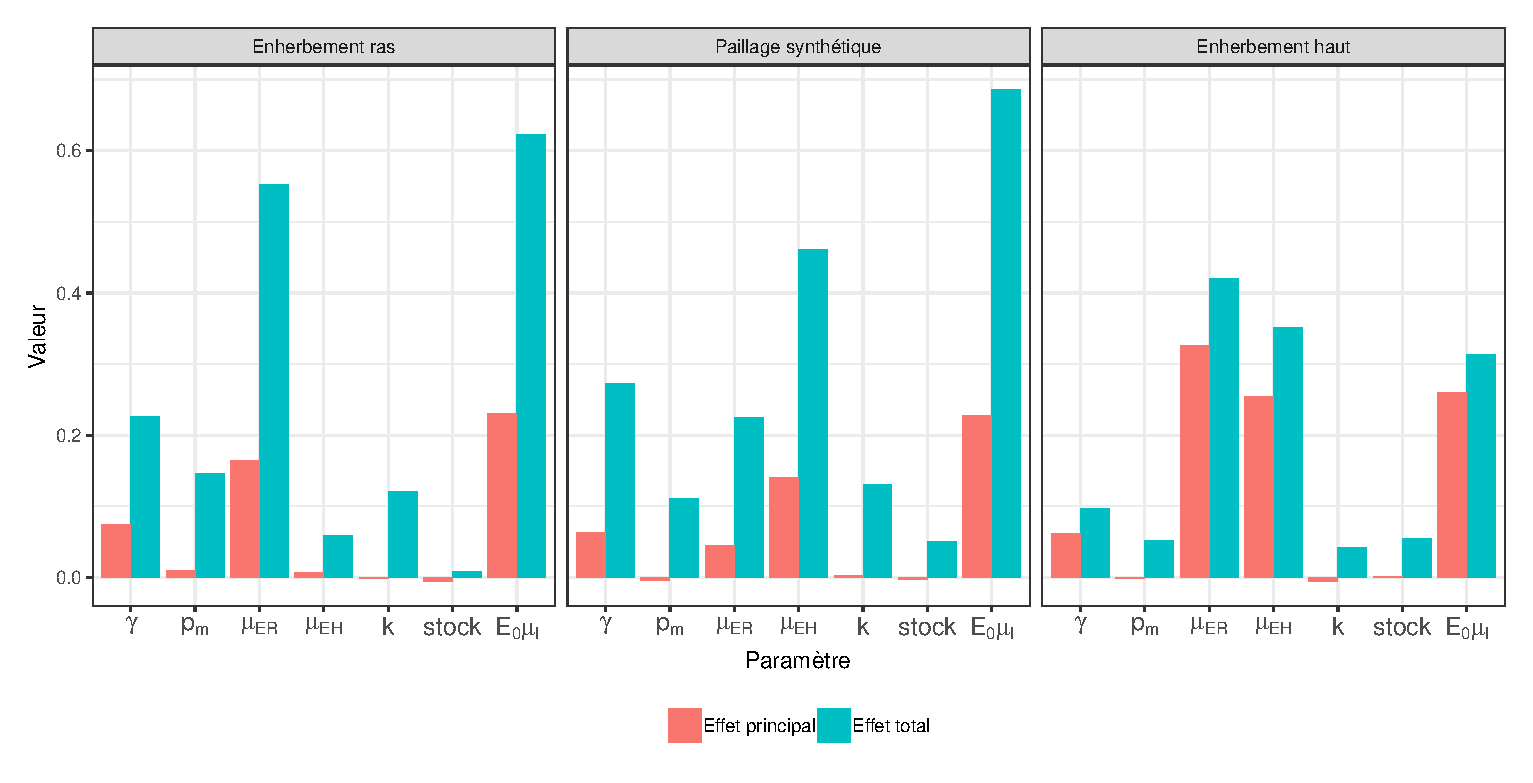
\epsfig{file = plots/sensitivity_analysis_A.eps, scale = 0.59}
 \caption{Analyse de sensibilité de notre modèle avec la méthode Sobol.}
 \label{fig:sa}
\end{figure}

On obtient ainsi les effets principaux et les effets totaux de Sobol pour chaque sous-parcelle.

Pour l'enherbement ras, le paramètre qui induit le plus de variance (effet principal) est $E_0\mu_\ell$ qui donne le nombre d'œufs arrivant au troisième stade de développement larvaire.
Sans surprise le probabilité de survie à la modalité de couverture du sol ER apporte aussi beaucoup de variance à cette sous-parcelle.
Ensuite, l'apport en variance du paramètre $\gamma$ n'est pas négligeable non plus.
En revanche, les quatre autres paramètres n'apportent en eux-même que peu de variance relativement aux trois autres nommés ci-dessus.
On remarque également que les paramètres qui apportent le plus de variance sont aussi ceux dont les interactions induisent le plus de variance.
(La variance apportée par les interactions d'un paramètre correspond à la différence entre l'effet total et l'effet principal).

Pour le paillage synthétique, c'est aussi $E_0\mu_\ell$ qui apporte le plus de variance.
Viennent ensuite $\mu_{\text{EH}}, \gamma$ et $\mu_{\text{ER}}$.
Les paramètres $p_{\text{m}}, k$ et \texttt{stock} n'apportent pas de variance.
Il est intéressant de noter que la probabilité de survie à la modalité de couverture du sol de la sous-parcelle EH a plus d'impact que celle de la sous-parcelle ER.
Ici aussi, ce sont les paramètres qui apportent le plus de variance qui ont le plus d'interactions.

Pour l'enherbement haut, c'est la probabilité de survie à la modalité de couverture du sol ER $\mu_{\text{ER}}$ qui apporte le plus de variance, ce qui est assez peu intuitif.
Il est suivi de près par deux autres paramètres : $\mu_{\text{EH}}$ et $E_0\mu_{\ell}$.
La part de variance apportée par le paramètre $\gamma$ n'est pas négligeable.
Celle apportée par $p_{\text{m}}, k$ et \texttt{stock} est négligeable.
Et une fois encore, ce sont les paramètres qui apportent le plus de variance qui ont le plus d'interactions.
% On s'aperçoit que le paramètre apportant le plus de variance à la sortie de notre modèle (effet principal) est $E_0\mu_\ell$, et ce pour chacune des trois sous-parcelles.
% Viennent ensuite les probabilités de survie à la modalité de couverture du sol.
% Sans surprise, le paramètre $\mu_{\text{EH}}$ apporte beaucoup de variance à la sous-parcelle avec la modalité de couverture de sol correspondante.
% De façon moins intuitive, ce paramètre apporte aussi beaucoup de variance à la sous-parcelle avec un enherbement haut.
% Il y apporte même plus de variance que le paramètre $\mu_{\text{EH}}$, bien que ce dernier en apporte aussi une part importante.
% Concernant la sous-parcelle avec un paillage synthétique, les probabilités de survie aux modalités de couverture du sol apporte aussi de la variance, avec un avantage pour $\mu_{\text{EH}}$.
% À noter que le paramètre $\gamma$ n'est pas en reste non plus, induisant une part non-négligeable de variance sur chacune des trois-sous-parcelles.
% Les paramètres $p_{\text{m}}, k$ et \texttt{stock} n'apportent en eux-mêmes que peu de variance.
% 
% On remarque également que les paramètres qui apportent le plus de variance sont aussi ceux dont les interactions induisent le plus de variance. (La variance apportée par les interactions d'un paramètre correspond à la différence entre l'effet total et l'effet principal).

Certains de ces résultats ne sont pas surprenants.
Il faut notamment se rappeler que le modèle est évalué sur l'estimation du nombre de larves, et que $E_0\mu_\ell$ intervient dans l'équation du modèle donnant le nombre de larves.
Ainsi, ce paramètre seul --- à valeur entre 1 et 11 --- peut facilement doubler le nombre de larves en fonction de sa valeur. Et induit donc naturellement une forte variance dans le modèle.
Et ce paramètre n'est interprétable que si l'on considère la valeur des autres paramètres.
Car un nombre élevé d'œufs pondus qui survivent peut être compensé par une faible probabilité de survie aux modalités de couverture de sol et une faible arrivée d'individus exogènes --- et vice-versa.
Ce qui peut expliquer ses fortes interactions.
Cette analyse de sensibilité montre surtout l'impact des probabilités de survie aux modalités de couverture du sol en fonction de chaque sous-parcelles, qui ne respecte pas ce que l'on pourrait s'imaginer \emph{a priori}.
On retiendra également que trois de nos paramètres ($p_{\text{m}}, k$ et \texttt{stock}) n'ont qu'un impact très limité --- comparativement aux autres --- sur la sortie du modèle.

\subsection{Calibration et choix des solutions}

En utilisant les mêmes intervalles pour les paramètres que ceux utilisés par l'analyse de sensibilité, on peut utiliser NSGA-II.
% pour obtenir un sous-ensemble du front de Pareto contenant des jeux de paramètres produisant des solutions non-dominées.
% L'algorithme est cependant stochastique, il ne renvoie jamais exactement deux fois les mêmes résultats.
% Pour pallier cet aspect, on exécute trente fois la fonction \texttt{nsga2} \citep{nsga} (avec une taille de population de 200, et 200 générations).
% Cela nous donne ainsi 6000 solutions. Mais parmi ces 6000 solutions certaines sont peut-être dominées par d'autres solutions provenant d'une exécution de \texttt{nsga2} différente.
% On ne récupère alors que les solutions non-dominées (et les jeux de paramètres correspondants) grâce à la fonction \texttt{is\textunderscore dominated} \citep{emoa}.
% Après avoir exécuté trente fois la fonction \texttt{nsga2} \citep{nsga} suivie de la fonction \texttt{is\textunderscore dominated} \citep{emoa} pour récupérer les solutions non-dominées.
% 
% on obtient ainsi 842 jeux de paramètres produisant autant de solutions non-dominées, parmi lesquelles on peut sélectionner des solutions.
% \subsection{Choix de solutions}
% On peut maintenant essayer de repérer différentes solutions--types reproduisant les quantités de larves observées.
% On effectue une CAH avec l'indice de Ward en utilisant la fonction \texttt{hclust} \citep{R}.
Parmi les 6000 solutions générées par la calibration du modèle avec l'algorithme d'optimisation NSGA-II, on a obtenu 842 jeux de paramètres produisant des solutions non-dominées.
Pour repérer par CAH les différentes solutions types parmi ces 842 solutions non-dominées, il faut dans un premier temps choisir un nombre de classes.
À cette fin, on regarde l'inertie intra-classes en fonction du nombre de classes (voir figure~\ref{fig:caha}).
Dans une optique de classification «classique», choisir 2, 3, 6 ou 8 classes pourrait s'avérer pertinent.
(Ces nombres de classes produisant une minimisation relativement importante de l'inertie intra-classes.)
Nous préférons cependant ne pas risquer de passer à côté d'une catégorie de solution potentiellement intéressante.
Nous choisirons 16 classes.

\begin{figure}[ht]
 \centering
 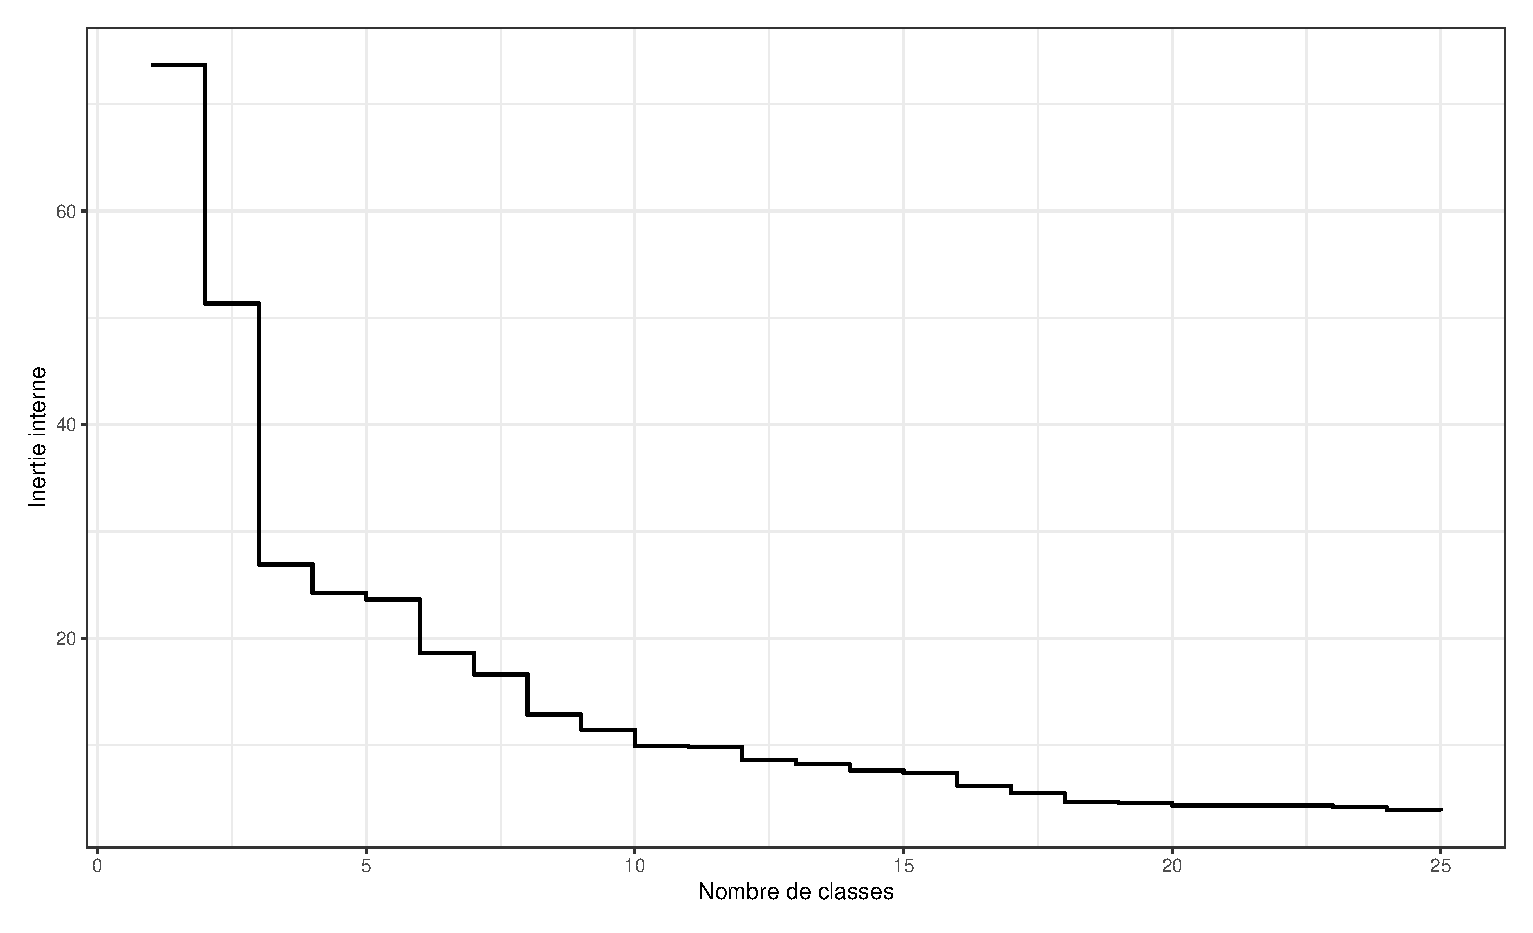
\epsfig{file = plots/cah_A.eps, scale = 0.55}
 \caption{Inertie intra-classes en fonction du nombres de classe obtenue par une CAH sur les jeux de paramètres renvoyés par NSGA-II.}
 \label{fig:caha}
\end{figure}


Parmi les 16 classes, trois solutions--types se distinguent.
Les solutions sont visibles sur la figure~\ref{fig:A1}.
On peut voir sur la figure la décomposition du nombre de larves en fonction de la provenance des femelles qui ont pondus les œufs.
Par exemple, si l'aire sous la courbe est essentiellement rouge, alors cela voudrait dire qu'il y a une forte proportion de femelles exogènes.
Et si elle est principalement verte, cela veut dire que la majorité des femelles qui pondent sont des femelles qui ont émergées dans une autre sous-parcelle. 
Cela peut questionner la pertinence biologique de la solution proposée, indépendamment de la qualité d'ajustement de la dynamique.

On détaille les trois solutions--types :
\begin{itemize}
 \item \textbf{Solution--type 1 :} 
 Les dynamiques pour les trois sous-parcelles sont grossièrement captées.
 Le modèle permet de simuler la présence plus précoce de cécidomyies sur la sous-parcelle ER et plus tardive sur les sous-parcelles PS et EH. 
 Il simule également un plus faible nombre de cécidomyies sur la sous-parcelle PS.
 Cependant le double pic caractérisant la dynamique des cécidomyies sur ER n'est pas capté, et la forte décroissance du nombre de cécidomyies en fin de saison est mal simulé.
 
 Les paramètres associées à ces trois dynamiques sont :
 \begin{center}
\begin{tabular}{lllllll}
$\gamma$ & $p_{\text{m}}$ & $\mu_{\text{ER}}$ & $\mu_{\text{EH}}$ & $k$ & \texttt{stock} & $E_0\mu_{\ell}$\\
0.08 & 0.494 & 0.976 & 0.046 & 1.928 & 5600 & 3.084
 \end{tabular}
 \end{center}
 Pour cette solution-type, on observe une quantité non négligeable de larves pondus par des femelles exogène (aire rouge), ce qui d'un point de vue biologique parait discutable.
L'absence d'individus qui émergent de la sous-parcelle EH s'explique par $\mu_{\text{EH}}$ qui est fixé à 0.046, ce qui veut dire que 95\% des larves meurent en essayant de s'enfouir dans la sous-parcelle ainsi que 95\% des femelles issues de pupaison ou de diapause qui essayent d'en émerger.
À la différence de la sous-parcelle ER où il n'y a pratiquement aucune mortalité induite par l'enherbement ras ($\mu_{\text{ER}} = 0.976$).
La valeur 0.8 attribuée à $\gamma$ est élevée (chose qui se confirmera empiriquement par les simulations qui suivront et qui peut déjà se voir sur la figure~\ref{fig:A1}).

\item \textbf{Solution--type 2 :} La qualité d'ajustement des dynamiques est assez similaire à celle de la première solution-type. Seule la décroissance en fin de saison est un peu mieux captée. Cependant, contrairement à la solution précédente qui avait trop d'individus exogènes, cette solution n'en a pas du tout.
On remarque également que les dynamiques des sous-parcelles PS et EH se composent uniquement de larves provenant d'œufs pondus par des femelles issues de la sous-parcelle ER.

Les paramètres sont :
 \begin{center}
\begin{tabular}{lllllll}
$\gamma$ & $p_{\text{m}}$ & $\mu_{\text{ER}}$ & $\mu_{\text{EH}}$ & $k$ & \texttt{stock} & $E_0\mu_{\ell}$\\
0 & 0.968 & 1 & 0.025 & 0.1 & 14483 & 6.26
 \end{tabular}
 \end{center}
 Ici aussi, il y a une absence totale d'individus qui émergent de la sous-parcelle avec un enherbement haut ($\mu_{\text{EH}} = 0.025$).
 L'absence d'individus exogènes se compensent par un nombre d'œufs pondus plus élevé que précédemment (6.26 contre 3.08) et un stock de larves diapausantes significatif (\texttt{stock} $=14483$).
 
\item \textbf{Solution--type 3 :}
Contrairement aux deux premières solutions, il y a ici des femelles qui émergent de la sous-parcelle EH.
Il faut cependant reconnaître que les dynamiques sont très mal captées : les problèmes d'ajustement des dynamiques identifiés pour les deux précédentes solutions sont toujours présents, et la décroissance en fin de saison est encore moins bien captée.

Les paramètres sont :
 \begin{center}
\begin{tabular}{lllllll}
$\gamma$ & $p_{\text{m}}$ & $\mu_{\text{ER}}$ & $\mu_{\text{EH}}$ & $k$ & \texttt{stock} & $E_0\mu_{\ell}$\\
0.026 & 0.93 & 0.565 & 0.647 & 0.174 & 13823 & 4.818
 \end{tabular}
 \end{center}
On observe que l'émergence d'individus dans la sous-parcelle EH ($\mu_{\text{EH}} = 0.647$ contre 0 précédemment) a entraîné une baisse d'émergence des individus dans la sous-parcelle ER ($\mu_{\text{ER}} = 0.565$ contre 0.97 et 1 pour les deux solutions précédentes)
 
\end{itemize}



\begin{figure}[ht]
 \centering
 \textbf{Solution--type 1}
 
 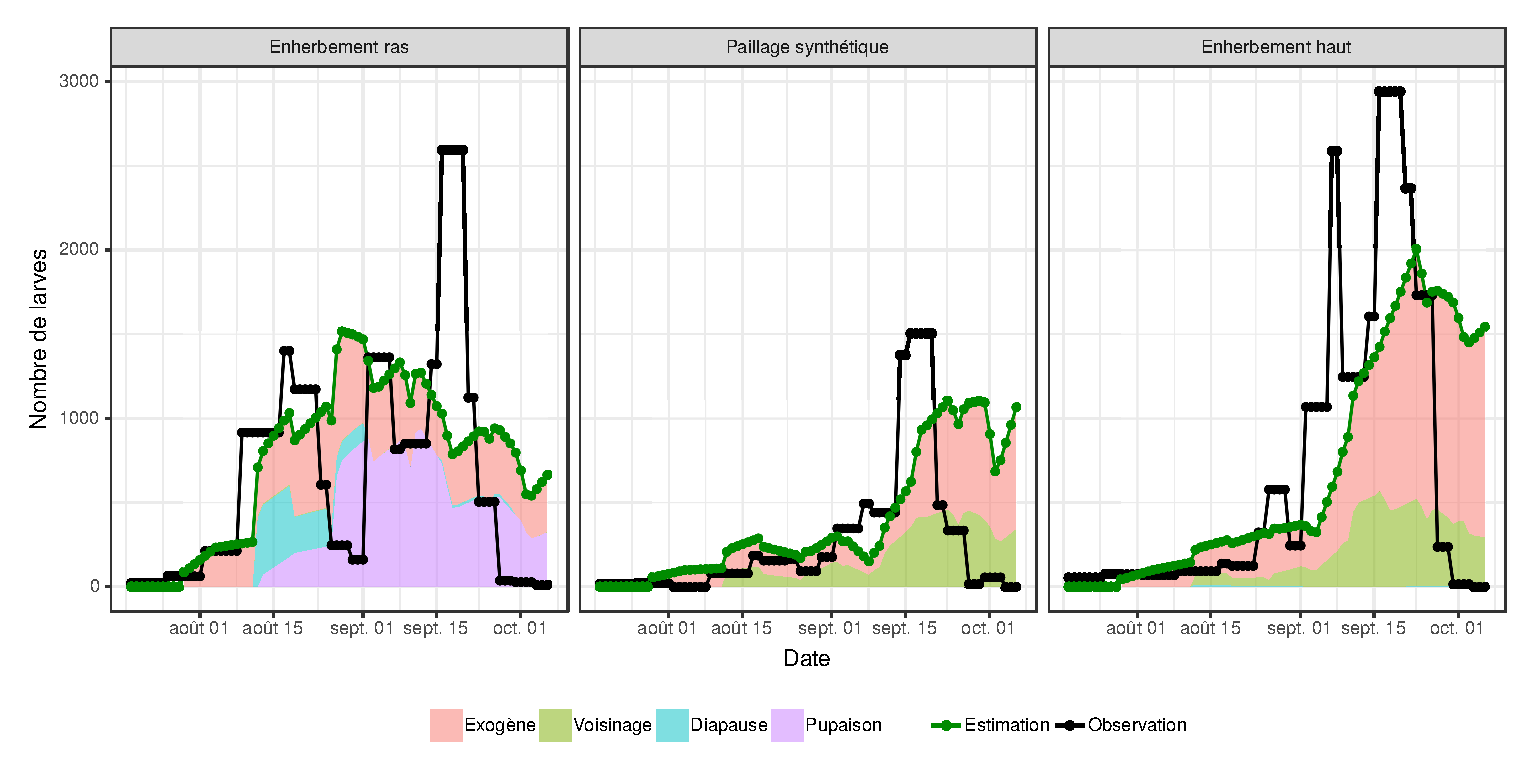
\epsfig{file = plots/A1.eps, scale = 0.52}
 
 \textbf{Solution--type 2}
 
 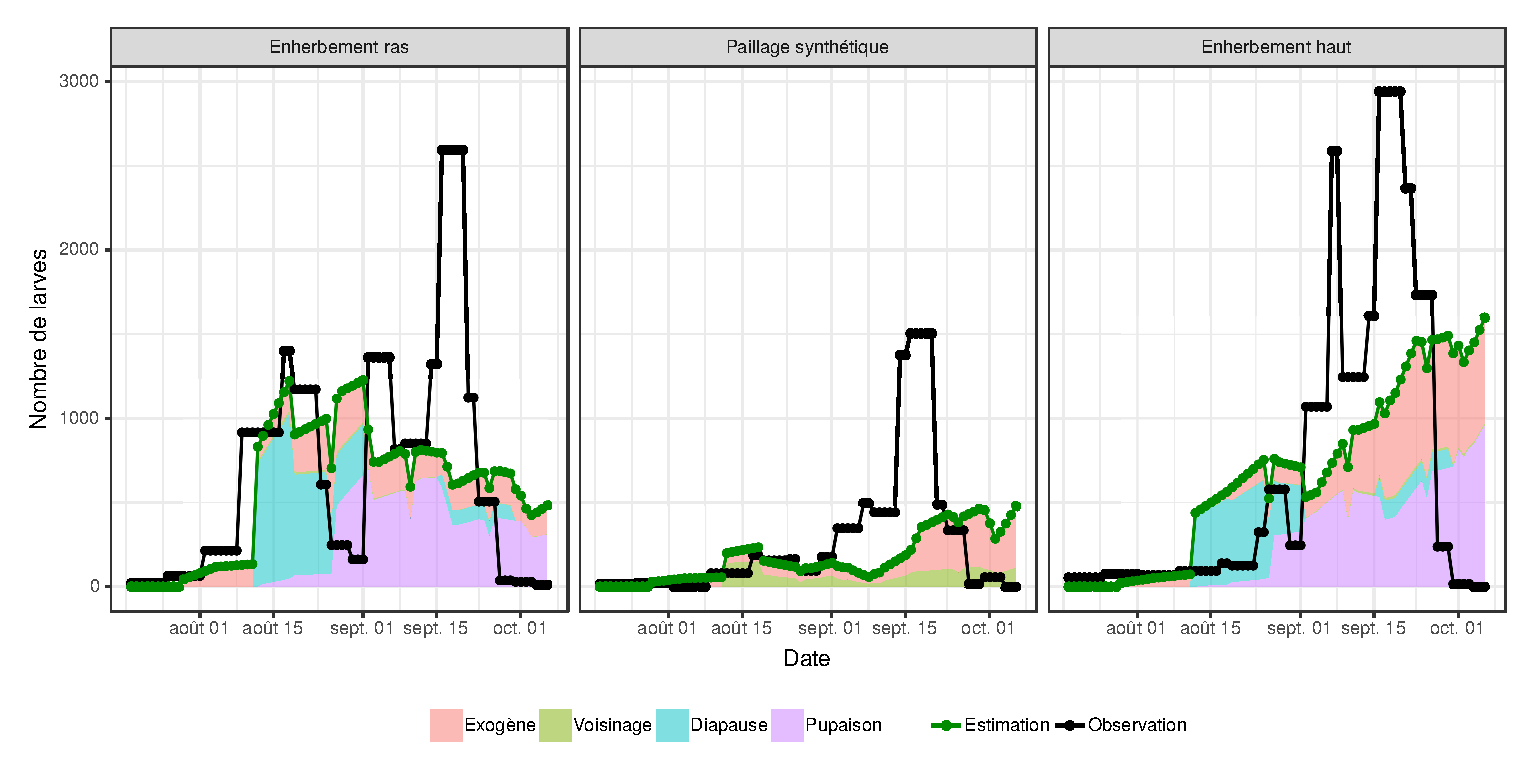
\epsfig{file = plots/A2.eps, scale = 0.52}
 
 \textbf{Solution--type 3}
 
 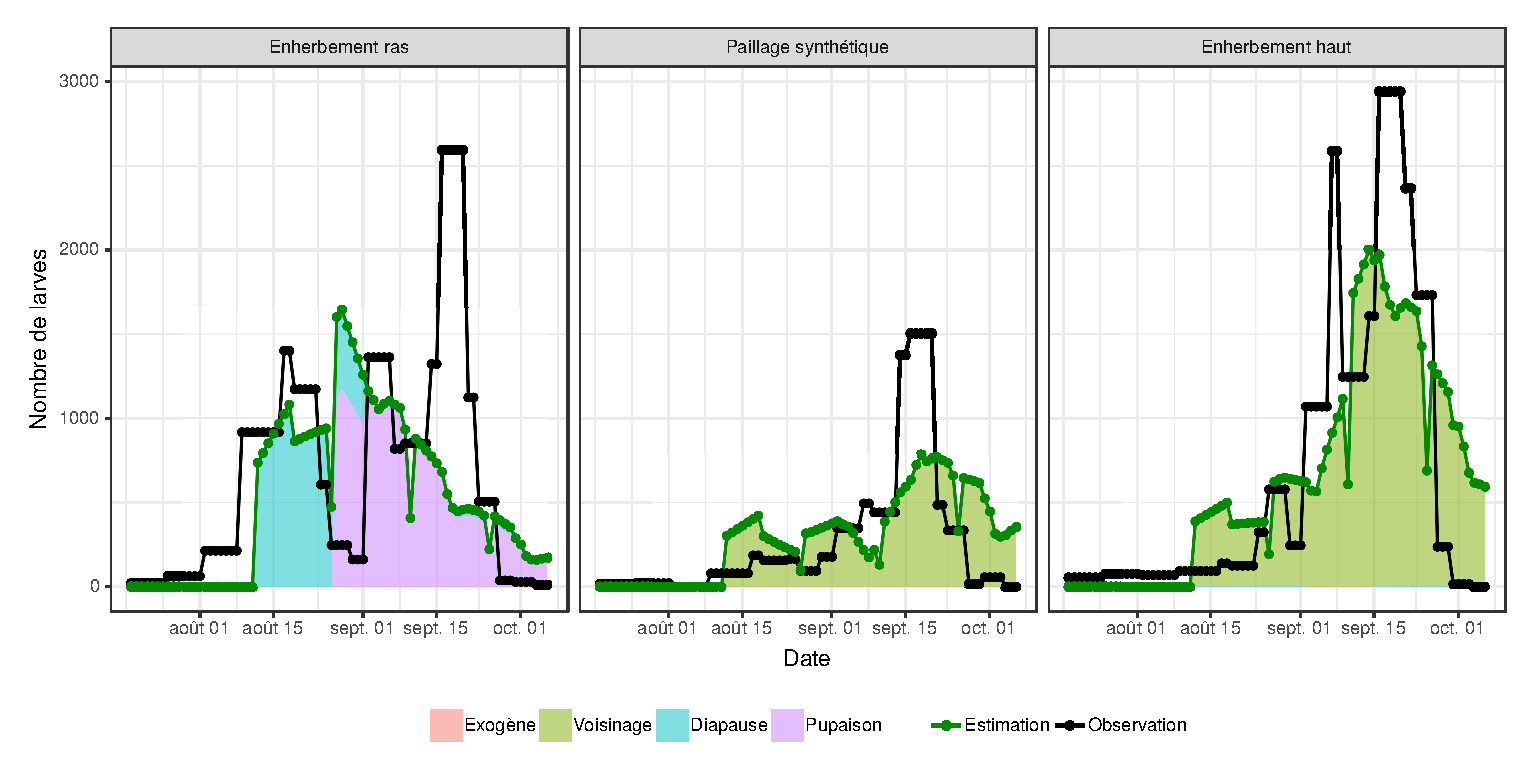
\epsfig{file = plots/A3.eps, scale = 0.52}
 \caption{Dynamiques observées et simulées pour chacune des trois solutions--types. La décomposition indiquant la provenance des femelles qui ont pondus les œufs est disponible pour les dynamiques simulées.}
 \label{fig:A1}
\end{figure}

Ces trois scénarios semblent tous montrer que le modèle actuel n'est pas suffisamment complet pour capter de façon satisfaisante le phénomène observé.
Pour les deux premières solutions, il y a quasiment aucun individus qui émergent de la sous-parcelle EH, et les individus se composent surtout d'individus exogènes (première solution-type) ou d'individus endogènes venant de la sous-parcelle ER (deuxième solution-type).
Et lorsqu'il y a des individus qui émergent de la sous-parcelle EH (troisième solution--type), le modèle ne parvient pas à recréer les dynamiques observées.

Cela peut s'expliquer par l'incapacité pour le modèle d'arrêter la reproduction des femelles et donc de stopper la dynamique en fin de saison induisant la baisse du nombre de larves observé.
C'est peut-être l'une des raisons pour laquelle le modèle fait appel  à beaucoup de femelles exogènes : elles sont proportionnelles aux inflorescences (dont la population baisse en fin de saison), ce qui entraîne donc une baisse du nombre de femelles et \emph{a fortiori} une baisse du nombre de larves.
Il y a dans le modèle un problème de décroissance en fin de saison.

Le modèle peut néanmoins être utilisé pour tester des hypothèses qui viendraient compléter ou remplacer les hypothèses initiales.
Et si en testant une de ces hypothèses, on trouve une solution qui permet d'ajuster convenablement les dynamiques et qui ne soit pas aberrante d'un point de vue biologique, on pourra alors essayer de valider la solution sur le verger n\textdegree2.


 
 \clearpage

\section{Solutions avec prise en compte de la température}
\label{chap:temp}

La première hypothèse à laquelle on s'intéresse est le lien entre la température et la probabilité d'entrer en pupaison.

On sait, d'après~\citet{pauldiap}, que la probabilité d'entrer en diapause et d'entrer en pupaison varie tout au long de l'année, et dépend de la température.
On espère ici qu'il y ait au cours de notre saison considérée (de juillet à octobre 2017) des variations de température pouvant expliquer une chute de la probabilité d'entrer en pupaison en fin de saison ce qui permettrait potentiellement au modèle de mieux reproduire la diminution du nombre de larves observées en fin de saison.

On choisira cependant la simplicité en essayant de trouver une relation linéaire permettant d'exprimer la probabilité d'entrer en pupaison en fonction de la température.
Pour réaliser ceci, on récupère les données de l'article de~\citet{pauldiap}.
Et à chaque taux de pupaison observé sur des larves prélevées en verger, on fait correspondre la température moyenne sur une quinzaine de jours (de 7 jours avant à 7 jours après la date du prélèvement).
On fait cela pour prendre en compte l'effet la température sur le cycle de développement complet de la cécidomyie --- depuis la ponte des œufs jusqu'à l'émergence des femelles issues de pupaison.


On effectue une régression linéaire simple de la probabilité d'entrer en pupaison en fonction de la température sur la quinzaine.
On fixera le seuil du risque de première espèce à $\alpha = 5\%$ pour le test de non-nullité des coefficients.
Les résultats sont visibles dans la table~\ref{tab:lm2}.

\begin{table}[hb]
\centering
\caption{Régression linéaire simple de la proportion d'individus en pupaison par la température moyenne sur 15 jours}
\label{tab:lm2}
\begin{tabular}{rrrrr}
 & Estimate & Std. Error & t value & Pr($>$$|$t$|$) \\ 
  \hline
(Intercept) & 1.9555 & 0.3665 & 5.34 & 0.0002 \\ 
  temp15j & -0.0550 & 0.0160 & -3.43 & 0.0050 \\ 
\end{tabular}
\end{table}

On en conclut que les coefficients associés à l'ordonnée à l'origine et à la température ne sont pas nuls et que l'on peut écrire
\[
p_{\text{p}} = 1.9555 - 0.055\times t_{15j}.
\]
La différence produite avec une probabilité constante fixée à 0.77, comme auparavant, est visible sur la figure~\ref{fig:pupaison}.
La différence en fin de saison est faible (environ 2\%), cela ne permettra pas \emph{a priori} d'améliorer le problème de la fin de saison.
En revanche, il y a des différences plus importantes au début de la saison de floraison qui pourraient peut-être améliorer l'ajustement général des dynamiques.

Les données utilisées proviennent d'observations effectuées en condition de laboratoire.
On laissera alors au modèle la possibilité d'amplifier la variation de la probabilité de pupaison afin de prendre en compte au mieux les conditions climatiques qu'il y aurait pu avoir sur le verger.
On peut faire ceci en utilisant la relation linéaire de la probabilité de pupaison en fonction de la température (donné ci-dessus par $p_{\text{p}}$) et un coefficient $\varpi\in [1;4]$ qui intervient comme suit :
\[
\widetilde p_{\text{p}} = \left( p_{\text{p}} - \overline{p_{\text{p}}} \right) \times \varpi + \overline{p_{\text{p}}},
\]
où $\widetilde p_{\text{p}}$ sera la probabilité d'entrer en pupaison et d'y survivre utilisée par le modèle et $\overline{p_{\text{p}}}$ la moyenne de la probabilité de pupaison.

\begin{figure}[ht]
 \centering
 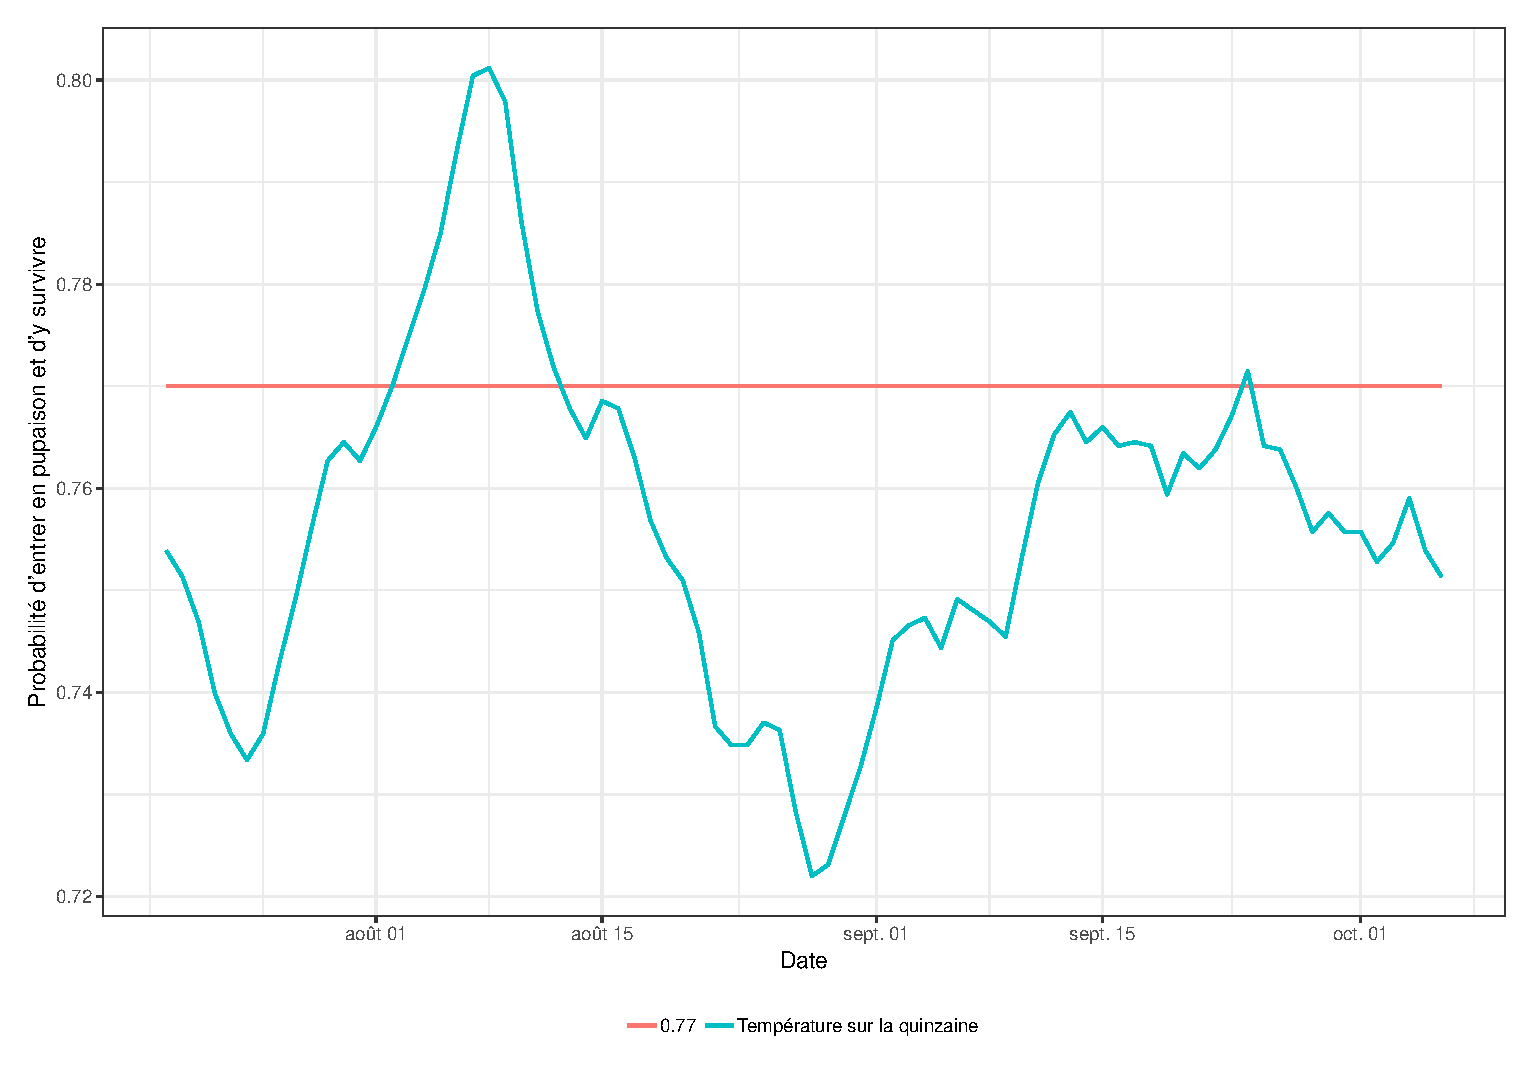
\epsfig{file = plots/pupaison.eps, scale = 0.55}
 \caption{Différence entre la probabilité d'entrer en pupaison et d'y survivre constante (égale à 0.77) et celle qui est fonction de la température moyenne sur la quinzaine.}
 \label{fig:pupaison}
\end{figure}
%

% Si l'on sait déjà que la température a un impact sur la sortie des individus en diapause, \citet{pauldiap} indique qu'elle a également un impact sur la probabilité d'entrer en pupaison.
% Intégrer cet aspect au modèle pourrait potentiellement permettre de réduire la reproduction de femelles endogènes en fin de saison, si la probabilité d'entrer en pupaison chute significativement.
% 
% On décide alors d'exprimer la probabilité d'entrer en pupaison et d'y survivre en fonction de la température.
% L'annexe~\ref{chap:pupaison} détaille la méthode utilisée.
% On se retrouve avec $p_{\text{p}}$ qui varie chaque jour et qui prend en compte la moyenne des températures quotidiennes sur quinze jours (de sept jours avant à sept jours après l'enfouissement).
% La différence produite avec une probabilité constante fixée à 0.77 est visible sur la figure~\ref{fig:pupaison}.
% 
% \begin{figure}[ht]
%  \centering
%  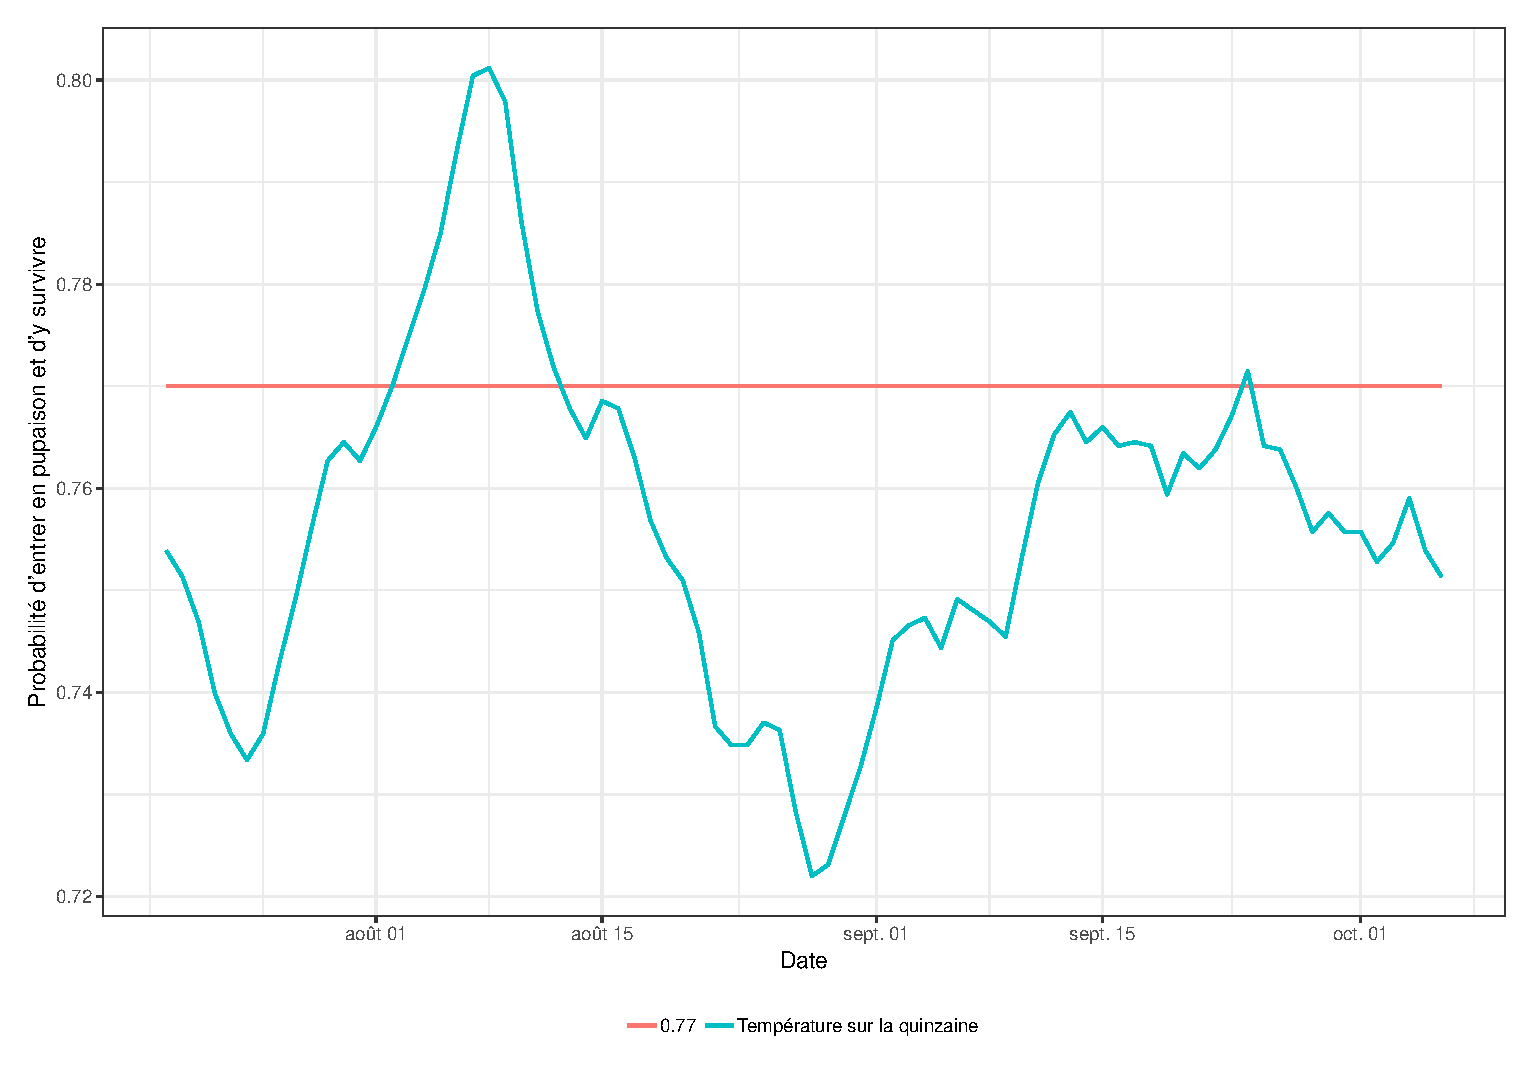
\epsfig{file = plots/pupaison.eps, scale = 0.55}
%  \caption{Différence entre la probabilité d'entrer en pupaison et d'y survivre constante (égale à 0.77) et celle qui est fonction de la température moyenne sur la quinzaine.}
%  \label{fig:pupaison}
% \end{figure}
% 
% On remarque peu de différences, c'est d'autant plus vrai en fin de saison où les deux probabilités sont très proches.
% Ce n'est donc pas l'effet de la température sur la phase de pupaison qui peut expliquer la diminution du nombre de larves observé en fin de saison.
% 
% On peut s'en convaincre en recalibrant le modèle avec cette nouvelle probabilité variable.
% On permet même au modèle «d'amplifier» la variabilité de la probabilité de pupaison en lui laissant le choix d'un certain coefficient $\varpi \in [1; 4]$ qui intervient comme suit :
% \[
% \widetilde p_{\text{p}} = \left( p_{\text{p}} - \overline{p_{\text{p}}} \right) \times \varpi + \overline{p_{\text{p}}},
% \]
% où $\widetilde p_{\text{p}}$ sera la probabilité d'entrer en pupaison et d'y survivre utilisée par le modèle.
% 
% Après obtention des résultats, on retrouve nos trois scénarios déjà présent dans la première version du modèle (voir figure~\ref{fig:B}).
% On peut noter que la calibration ne renvoie pas de valeur de $\varpi$ supérieure à 1.5, montrant que des variations dans la probabilité de rentrer en pupaison n'aide pas à améliorer l'ajustement des dynamiques.

Après calibration du modèle et classification des solutions, on trouve trois solutions--types, qui sont très similaires à celles trouvées avec le modèle initial.
Les voici :
\begin{itemize}
 \item \textbf{Solution--type 1 :} 
 Une solution faisant appel à beaucoup d'individus exogènes et sans individus qui émergent de la sous-parcelle EH.
 
 Les paramètres sont :
 \begin{center}
\begin{tabular}{llllllll}
$\gamma$ & $p_{\text{m}}$ & $\mu_{\text{ER}}$ & $\mu_{\text{EH}}$ & $k$ & \texttt{stock} & $E_0\mu_{\ell}$ & $\varpi$\\
0.044 & 0.715 & 0.998 & 0.002 & 0.143 & 1548 & 4.202 & 1.167
 \end{tabular}
 \end{center}

\item \textbf{Solution--type 2 :} 
Une solution sans individus exogènes ni sans individus qui émergent de la sous-parcelle EH.

Les paramètres sont :
 \begin{center}
\begin{tabular}{llllllll}
$\gamma$ & $p_{\text{m}}$ & $\mu_{\text{ER}}$ & $\mu_{\text{EH}}$ & $k$ & \texttt{stock} & $E_0\mu_{\ell}$ & $\varpi$\\
0.000 & 1 & 1 & 0.001 & 0.1 & 17188 & 6.3 & 1.036
 \end{tabular}
 \end{center}
 
\item \textbf{Solution--type 3 :}
Une solution avec des femelles qui émergent de la sous-parcelle EH  et sans individus exogènes.

Les paramètres sont :
 \begin{center}
\begin{tabular}{llllllll}
$\gamma$ & $p_{\text{m}}$ & $\mu_{\text{ER}}$ & $\mu_{\text{EH}}$ & $k$ & \texttt{stock} & $E_0\mu_{\ell}$ & $\varpi$\\
0.002 & 0.280 & 0.923 & 0.986 & 0.177 & 20066 & 3.288 & 1.110
 \end{tabular}
 \end{center}
\end{itemize}

Il n'est probablement pas très pertinent de s'étendre longuement sur ces trois nouvelles solutions, dans la mesure où elles sont très similaires aux solutions trouvées avec le modèle initial.
On peut remarquer que le paramètre $\varpi$ ne dépasse jamais 1.5, ce qui semble indiquer que la prise en compte de l'effet de la température sur la probabilité d'entrer en pupaison ne semble pas améliorer le modèle.

La température n'explique pas le phénomène observé en fin de saison pour l'année de 2017, les températures ne changeant pas suffisamment entre le début et la fin de cette saison.
Il se peut néanmoins qu'il y ait certaines saisons où les écarts de températures soient suffisamment importants pour qu'il faille les prendre en compte.
C'est pourquoi on gardera par la suite la prise en compte de la température sur la probabilité d'entrer en pupaison, en fixant $\varpi = 1.$ 

On s'intéresse également dans l'annexe~\ref{chap:pup_chelou} au cas où le modèle a plus de liberté pour l'ajustement de la probabilité d'entrer en phase de pupaison.

\begin{figure}[h]
 \centering
 \textbf{Solution--type 1}
 
 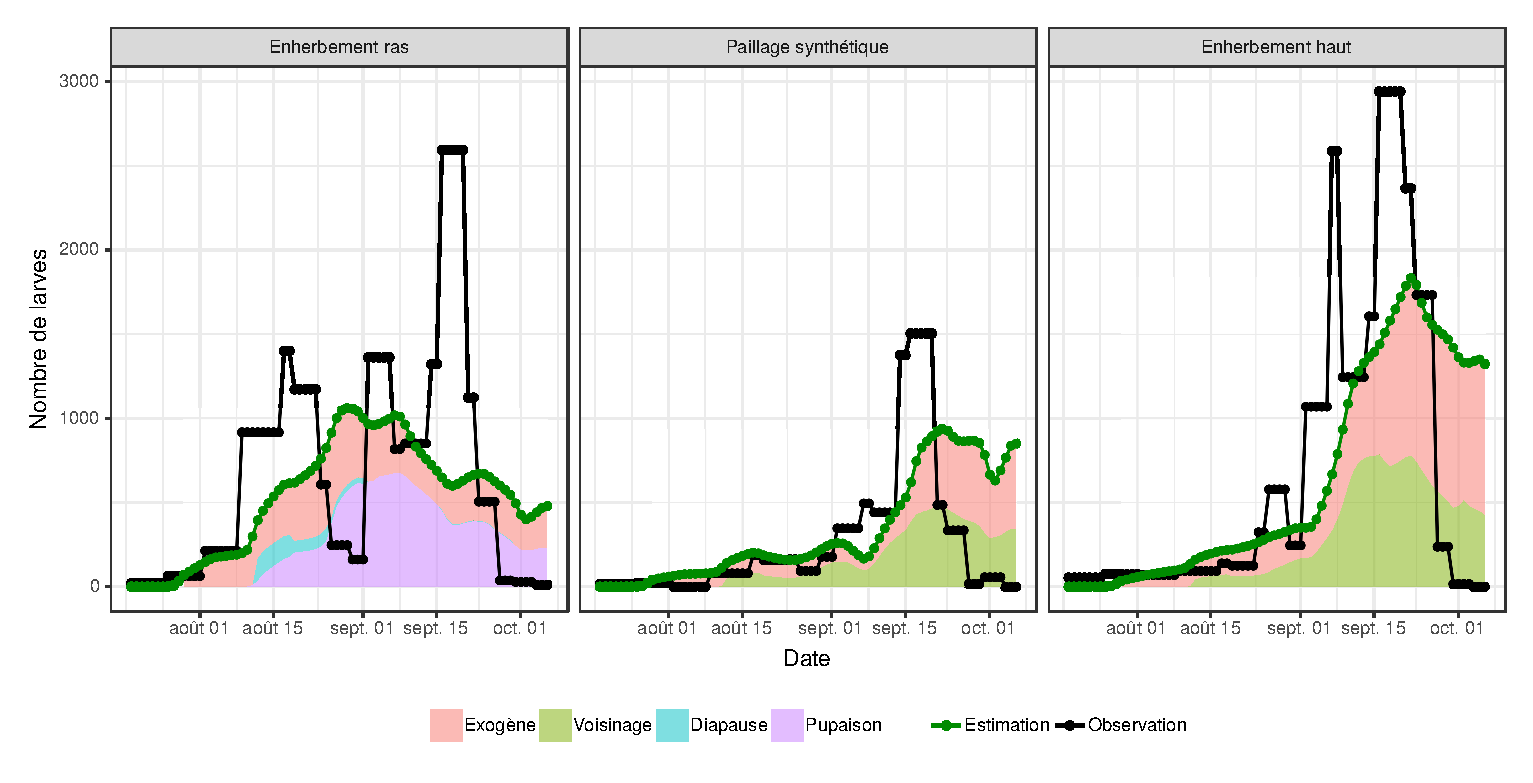
\epsfig{file = plots/B1.eps, scale = 0.52}
 
 \textbf{Solution--type 2}
 
 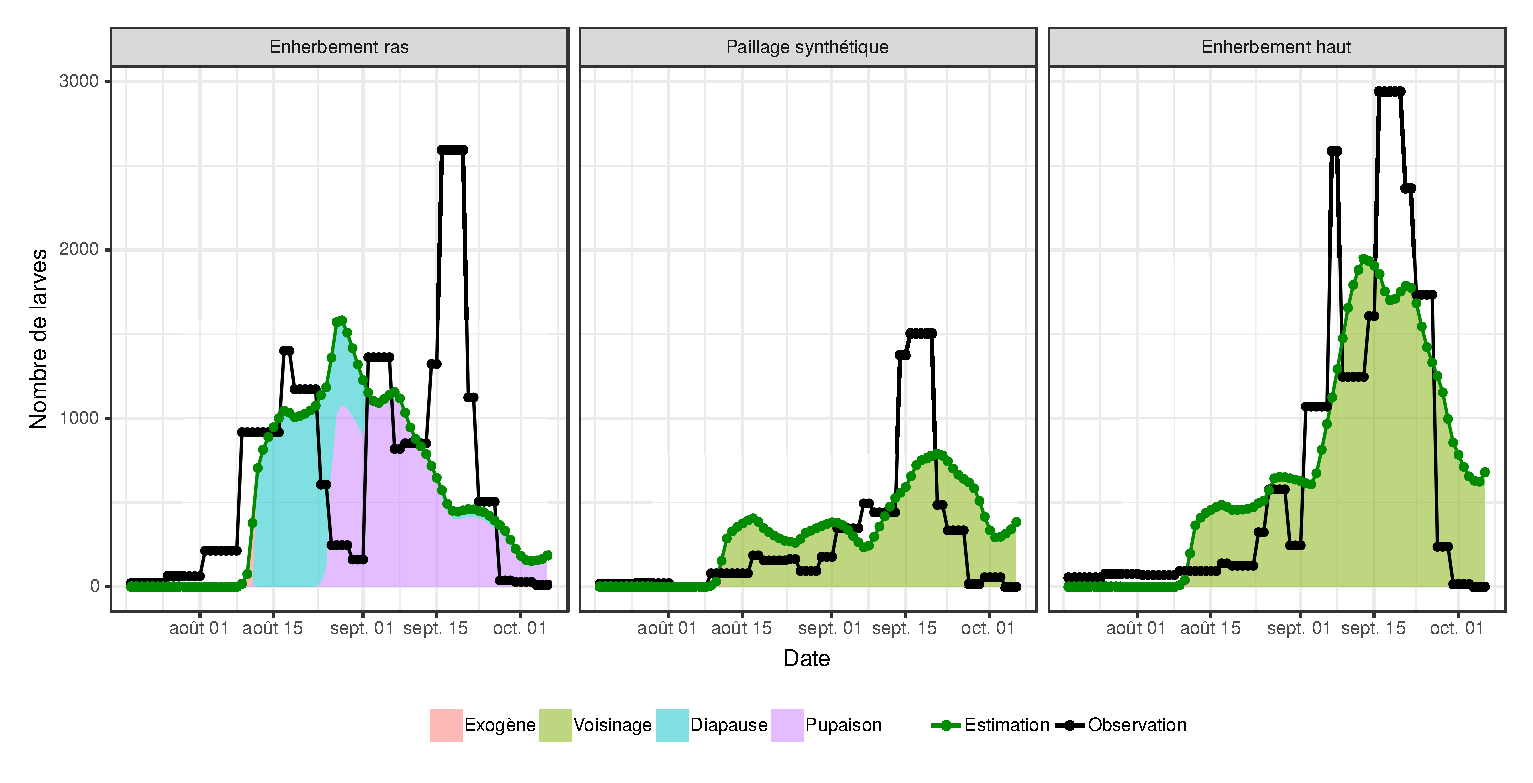
\epsfig{file = plots/B2.eps, scale = 0.52}
 
 \textbf{Solution--type 3}
 
 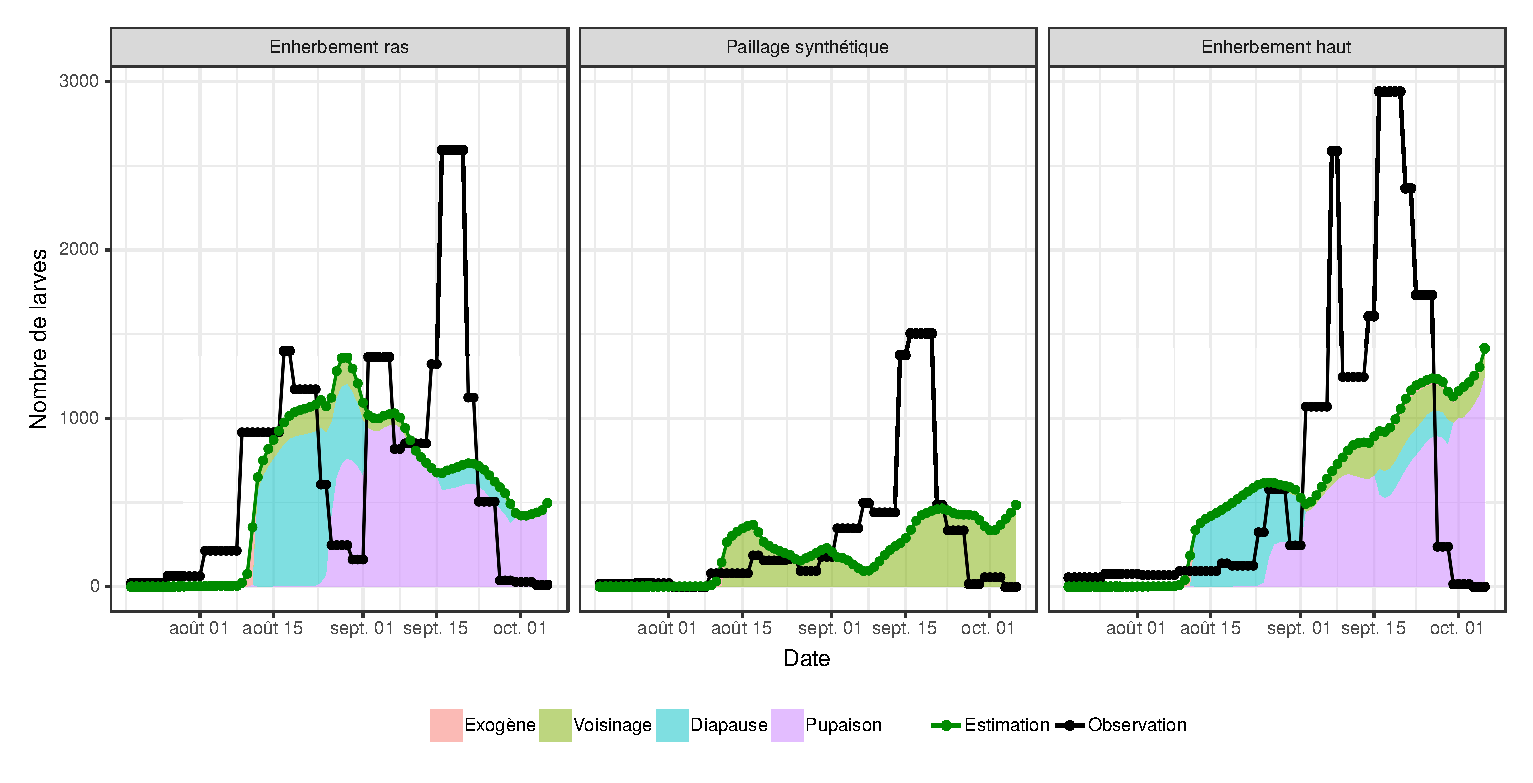
\epsfig{file = plots/B3.eps, scale = 0.52}
 \caption{Dynamiques observées et simulées pour chacune des trois solutions--types. La décomposition indiquant la provenance des femelles qui ont pondus les œufs est disponible pour les dynamiques simulées.}
 \label{fig:B}
\end{figure}

\clearpage
\section{Solutions avec prise en compte de contraintes liées aux ressources}
\label{chap:cde}

Puisque la température n'explique pas le phénomène observé en fin de saison, on teste une autre hypothèse.
On s'intéresse aux ressources.
L'intérêt pour les ressources est motivé par le fait que, sur les figures~\ref{fig:larves} et~\ref{fig:larves2}, les dynamiques de larves semblent corrélées avec les dynamiques d'inflorescences vivantes.
Les coefficients de corrélations de Spearman (du verger n\textdegree1) confirment plus ou moins cette intuition :
\[
\rho^{\text{ER}}\left( L_t, I_t  \right) =0.46,  \qquad \rho^{\text{PS}}\left( L_t, I_t  \right) =0.68, \qquad \rho^{\text{EH}}\left( L_t, I_t  \right) =0.76.
\]
On pourrait s'attendre à un décalage entre les dynamiques de larves et d'inflorescences, correspondant à la durée de développement qu'il faut entre la ponte et l'apparition du troisième stade larvaire.
Or, sur les figures~\ref{fig:larves} et~\ref{fig:larves2}, cela ne s'observe pas.

Pour expliquer cette absence de décalage, on émet une hypothèse.
Une inflorescence n'est pas attractive pour une cécidomyie de son débourrement jusqu'à la fin de sa vie mais uniquement lors des premiers stades phénologiques de l'inflorescence.
Lorsqu'elle atteint le stade phénologique F, la tige se durcit progressivement, rendant peut-être plus difficile la ponte pour les cécidomyies.
Notre hypothèse est que seules les inflorescences aux stades phénologiques C, D et E sont considérées comme attractives par les cécidomyies.

On détaille dans l'annexe~\ref{chap:deb} comment nous sommes capables de simuler des dynamiques d'inflorescences aux stades C, D et E.

Nous ferons ici l'hypothèse que la durée d'attractivité est de seize jours, ce qui correspond à la durée théorique des stades phénologiques C, D et E.
La différence entre les inflorescences vivantes et les inflorescences attractives est visible sur la figure~\ref{fig:CDE}.

\begin{figure}[ht]
 \centering
 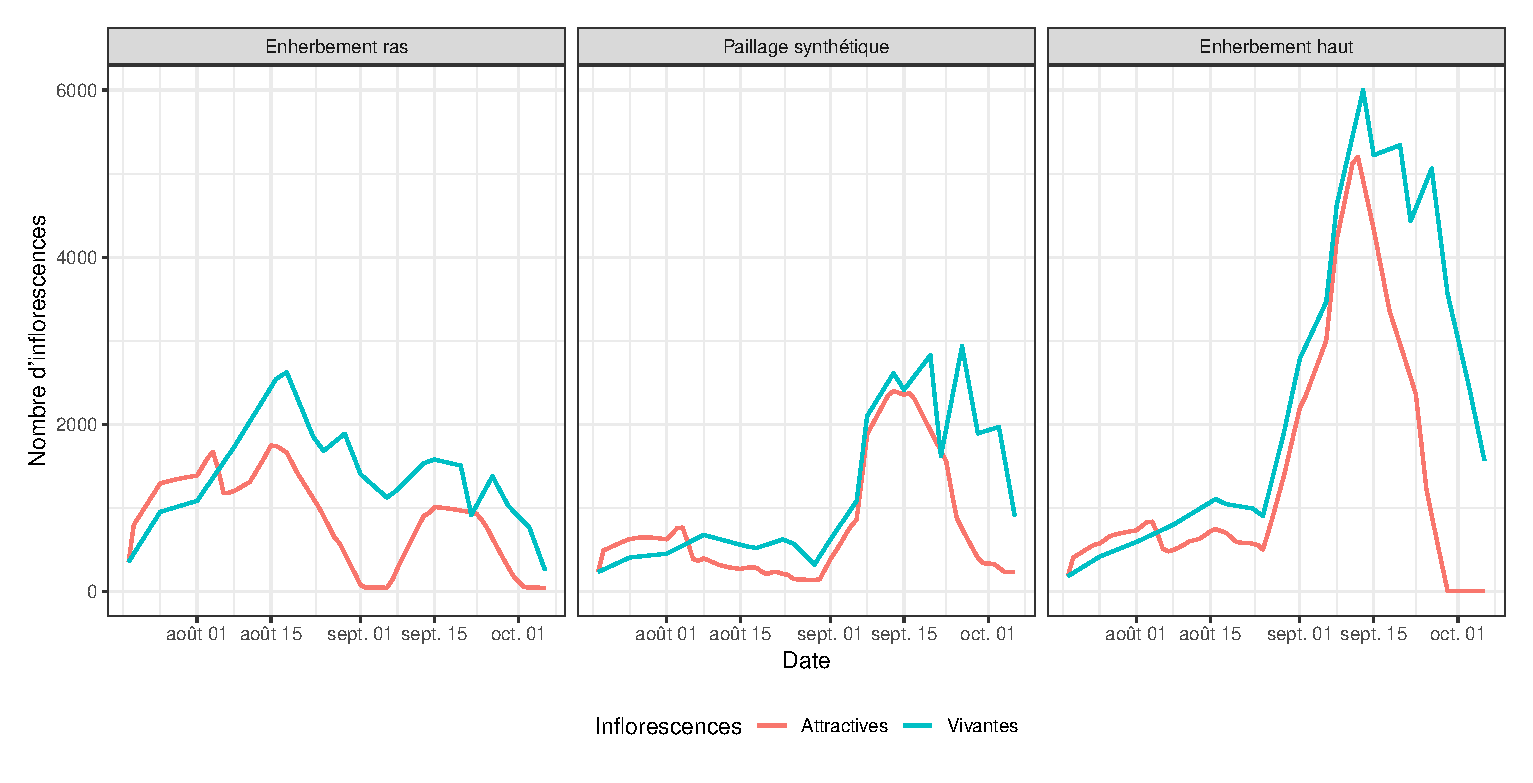
\epsfig{file = plots/inflos_CDE.eps, scale = 0.53}
 \caption{Différence entre les inflorescences vivantes et les inflorescences attractives.}
 \label{fig:CDE}
\end{figure}


Sur les trois solutions--types trouvées après la calibration du modèle, deux correspondent à celles trouvées précédemment.
Les dynamiques sont visibles sur la figure~\ref{fig:C}.
On observe une amélioration sur les sous-parcelles PS et EH, notamment en ce qui concerne la fin de dynamique en fin de saison.
La parcelle ER est en revanche toujours mal captée.
Et la pertinence biologique des solutions (concernant la forte présence ou l'absence d'individus exogènes et l'absence d'individus qui émergents de la sous-parcelle EH) reste toujours discutable.

Les paramètres pour les trois solutions--types sont les suivants :
{%
\newcommand{\mc}[3]{\multicolumn{#1}{#2}{#3}}
\begin{center}
\begin{tabular}{lllllll}
\mc{7}{c}{\textbf{Solution--type 1}}\\
$\gamma$ & $p_{\text{m}}$ & $\mu_{\text{ER}}$ & $\mu_{\text{EH}}$ & $k$ & \texttt{stock} & $E_0\mu_\ell$\\
0.115 & 0.189 & 0.898 & 0.012 & 1.877 & 515 & 3.097\\
 &  &  &  &  &  & \\
\mc{7}{c}{\textbf{Solution--type 2}}\\
$\gamma$ & $p_{\text{m}}$ & $\mu_{\text{ER}}$ & $\mu_{\text{EH}}$ & $k$ & \texttt{stock} & $E_0\mu_\ell$\\
0.004 & 0.490 & 0.990 & 0.018 & 0.242 & 9970 & 5.638\\
 &  &  &  &  &  & \\
\mc{7}{c}{\textbf{Solution--type 3}}\\
$\gamma$ & $p_{\text{m}}$ & $\mu_{\text{ER}}$ & $\mu_{\text{EH}}$ & $k$ & \texttt{stock} & $E_0\mu_\ell$\\
0.000 & 0.094 & 0.999 & 0.514 & 0.181 & 18214 & 8.259
\end{tabular}
\end{center}
}%


\begin{figure}[ht]
 \centering
 
  \centering
 \textbf{Solution--type 1}
 
 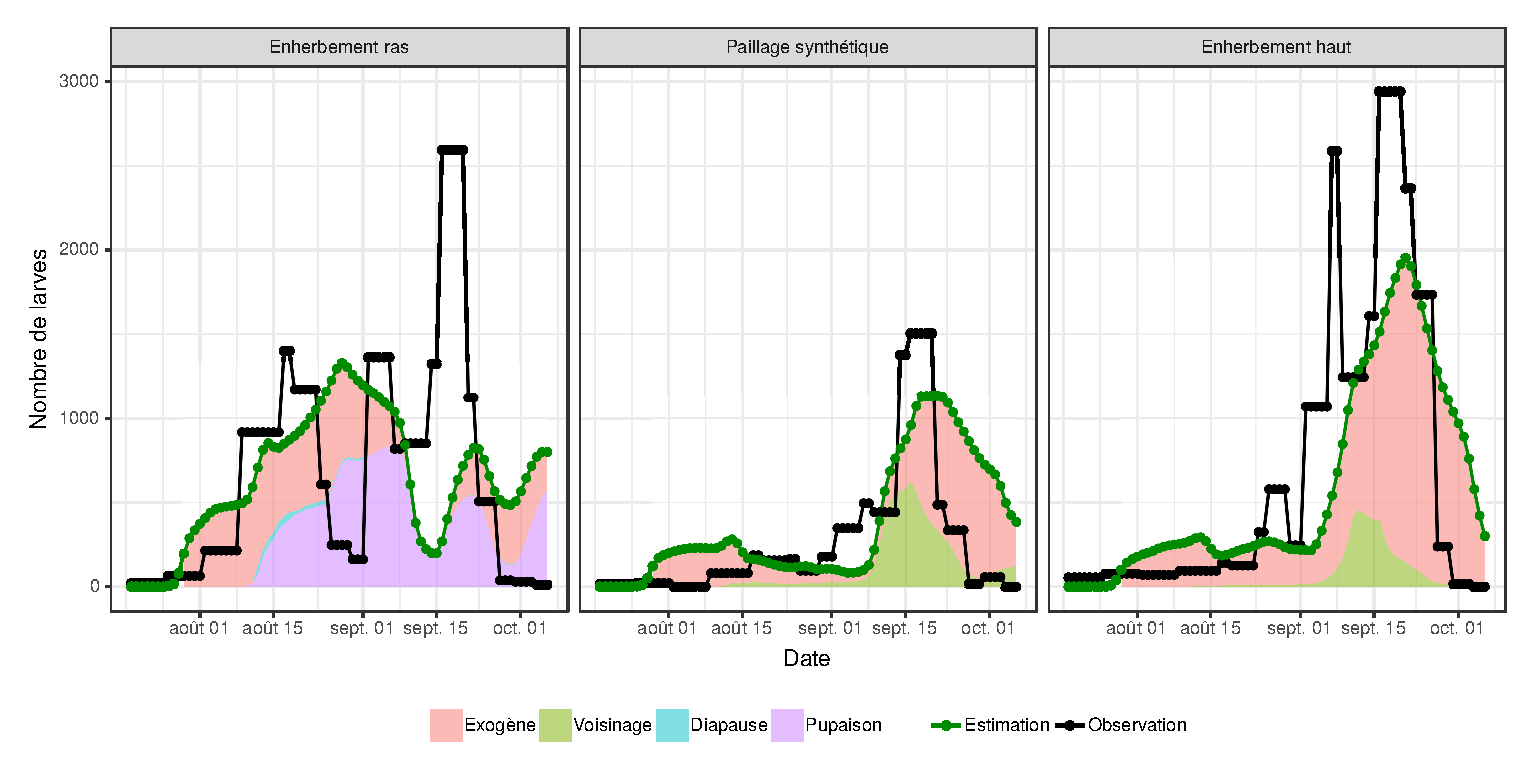
\epsfig{file = plots/C1.eps, scale = 0.52}
 
 \textbf{Solution--type 2}
 
 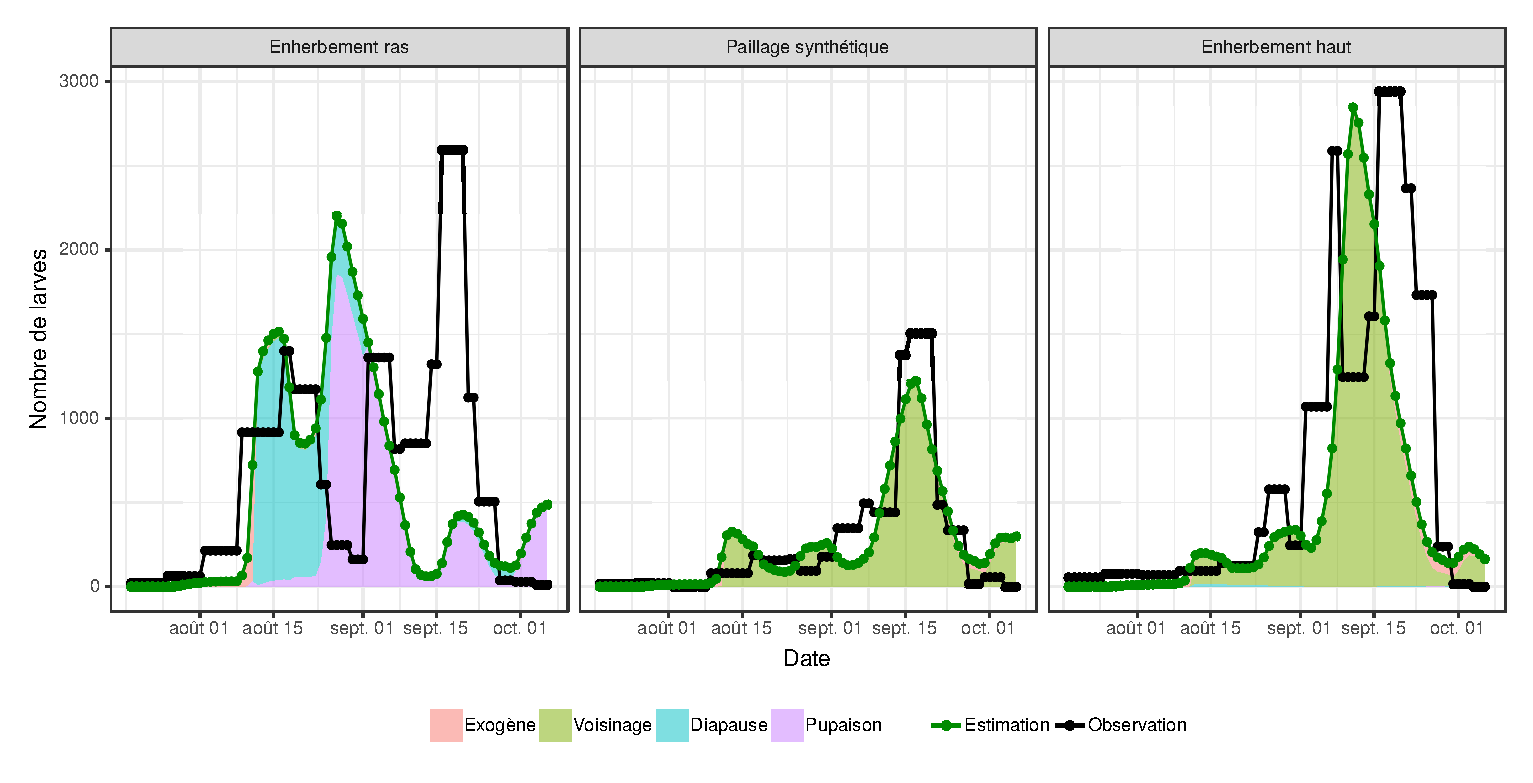
\epsfig{file = plots/C2.eps, scale = 0.52}
 
 \textbf{Solution--type 3}
 
 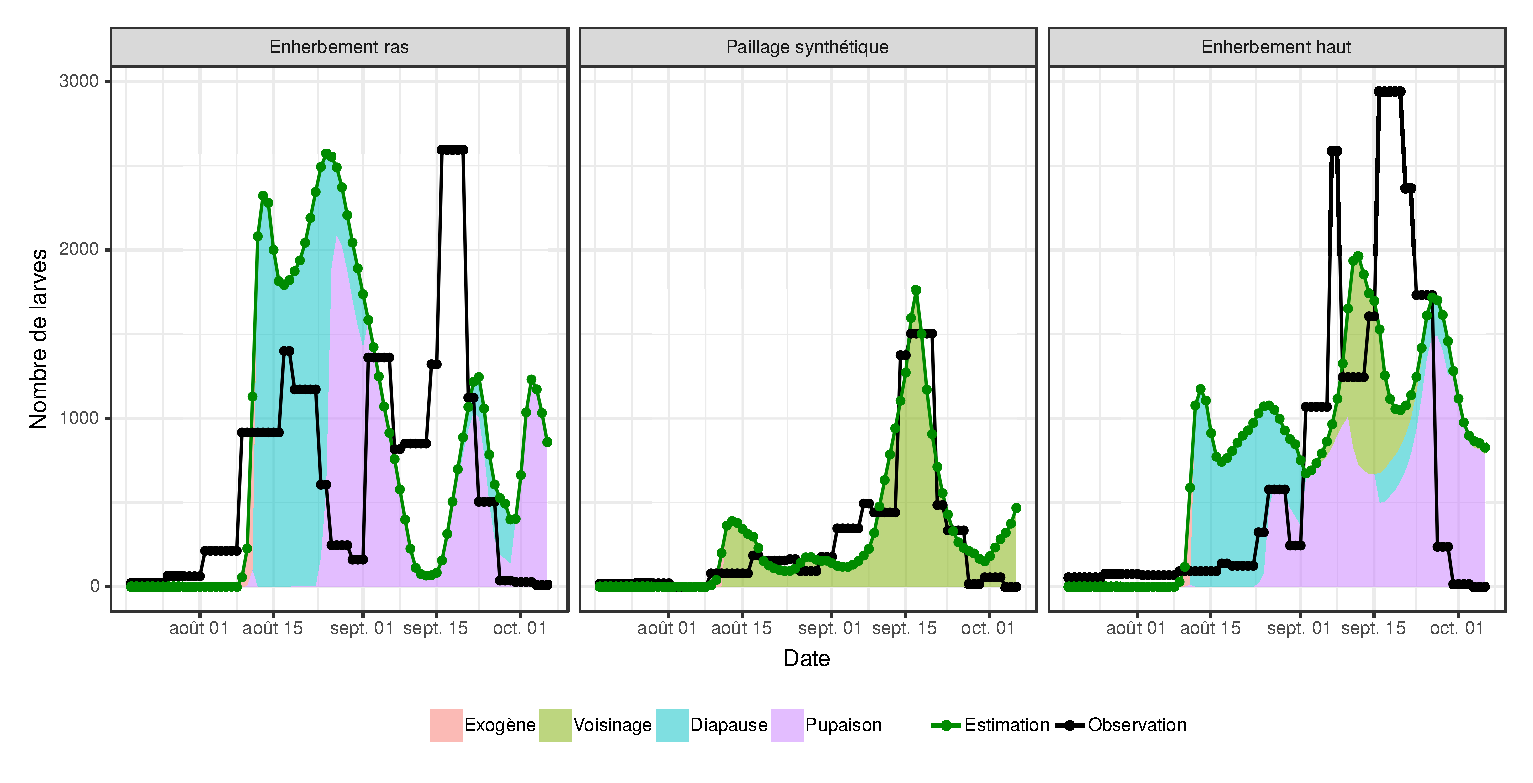
\epsfig{file = plots/C3.eps, scale = 0.52}
 
 
 \caption{Dynamiques observées et simulées pour chacune des trois solutions--types. La décomposition indiquant la provenance des femelles qui ont pondus les œufs est disponible pour les dynamiques simulées.}
 \label{fig:C}
\end{figure}


On remarquera que la prédiction sur la troisième solution--type est toujours aussi mauvaise.
La prise en compte de l'attractivité des inflorescences ne permet toujours pas la baisse des dynamiques observées en fin de saison lorsqu'il y a des individus endogènes dans la sous-parcelle EH.

Le choix d'une durée attractive de seize jours correspondant à la durée des stades phénologiques C, D et E peut apparaître comme un choix trop arbitraire.
On traite dans l'annexe~\ref{chap:attra} le cas où le modèle calibre aussi la durée d'attractivité.

\clearpage
\section{Solutions avec l'introduction d'un paramètre de saisonnalité}

Les hypothèses émises jusqu'à présent n'ont pas permis d'expliquer ce qu'il se produit en fin de saison.
Aux hypothèses déjà faites (probabilité d'entrer en phase de pupaison dépendant de la température et durée d'attractivité des inflorescences de 16 jours), on en rajoute une autre.
Ce que l'on observe sur les dynamiques de larves, c'est qu'il semble y avoir une forte baisse de la population de larves qui s'amorce aux alentours du 15 septembre (sur le verger n\textdegree1).
On émet alors l'hypothèse qu'un phénomène intervient à cette date.
Ce phénomène non-observé caractériserait un changement de la conjoncture sur le verger et induirait une baisse du nombre de larves.

Et on modélise cette hypothèse de manière radicale en introduisant un paramètre de saisonnalité $\xi \in [0;1]$ sur le nombre de femelles dans le verger à partir du 15 septembre.
Cela donne en pratique
\[
F_{t,i} := \begin{cases}
            F_{t, i} & \text{si $t<$ 15 septembre,}\\
            \xi \, F_{t, i} & \text{si $t\geq$ 15 septembre.}
           \end{cases}
\]
Concrètement, si le modèle décide de mettre une valeur éloignée de 1, cela signifie qu'à partir du 15 septembre que le cycle de développement de la cécidomyie subit des perturbations qui entraînent une baisse du nombre de larves produites.

Après calibration du modèle, un scénario se dégage des autres.
Il est visible sur la figure~\ref{fig:D}.
Les paramètres associés sont les suivants :
\begin{center}
\begin{tabular}{llllllll}
$\gamma$ & $p_{\text{m}}$ & $\mu_{\text{ER}}$ & $\mu_{\text{EH}}$ & $k$ & \texttt{stock} & $E_0\mu_{\ell}$ & $\xi$\\
0.021 & 0.105 & 0.938 & 0.916 & 1.992 & 516 & 6.018 & 0.004
\end{tabular}
\end{center}


\begin{figure}[ht]
 \centering
 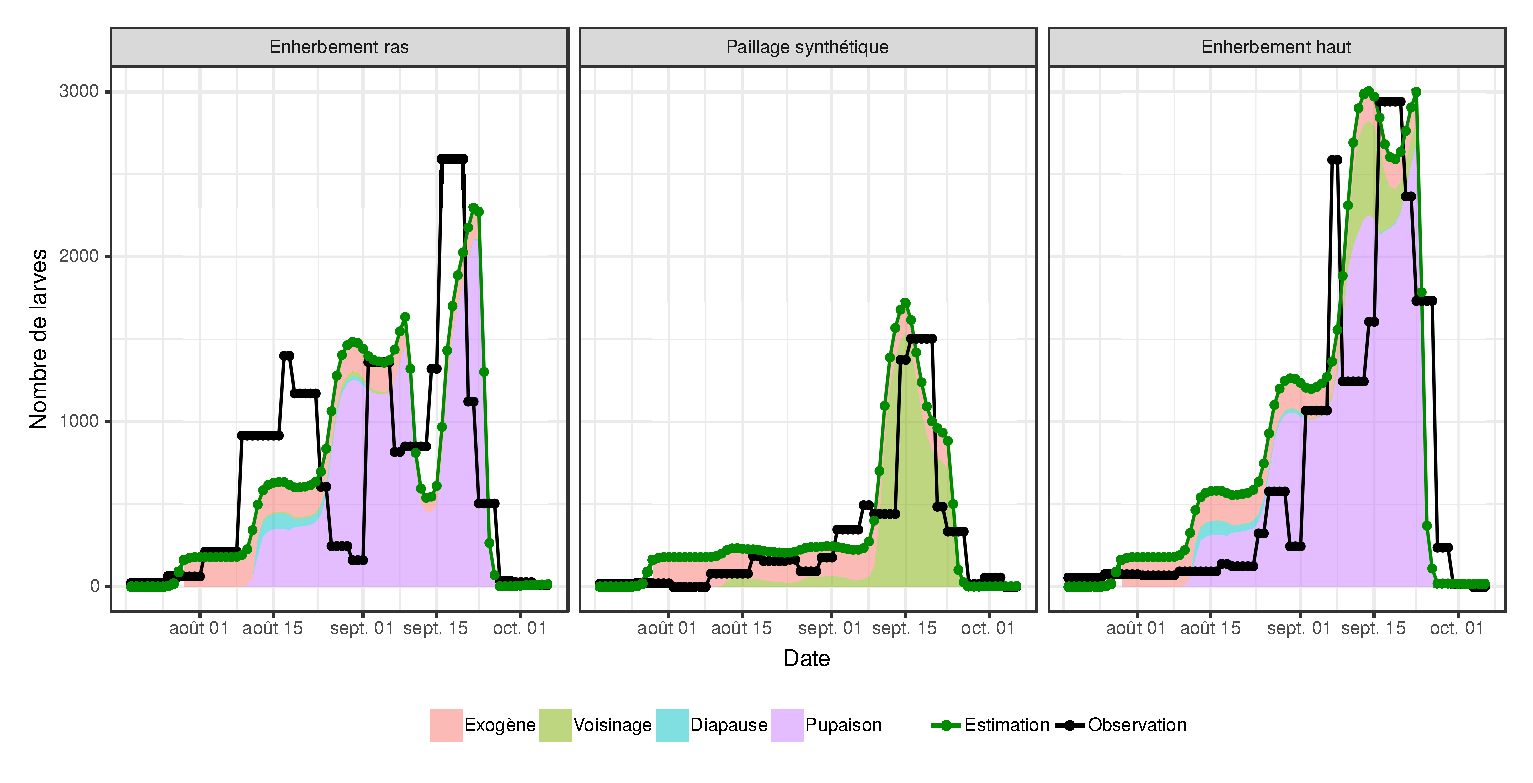
\epsfig{file = plots/D1.eps, scale = 0.59}
 \caption{Dynamiques observées et simulées. La décomposition indiquant la provenance des femelles qui ont pondus les œufs est disponible pour les dynamiques simulées.}
 \label{fig:D}
\end{figure}


Les dynamiques sont ici très bien captées pour les sous-parcelles PS et EH.
La dynamique de la sous-parcelle ER est plutôt bien captée, surtout si l'on relativise vis à vis des des estimations précédentes qui ont toujours étés mauvaises.
Les paramètres montrent (et le graphique aussi) qu'il y a principalement des femelles endogènes, ce qui semble vraisemblable.



Cela semble être une bonne estimation.
On procède à la validation sur le verger n\textdegree2.
Les résultats obtenus sont visibles sur la figure~\ref{fig:vg2_15s}.
Les prédictions sont plutôt mauvaises tant en terme d'intensité que de temporalité.

\begin{figure}[ht]
 \centering
 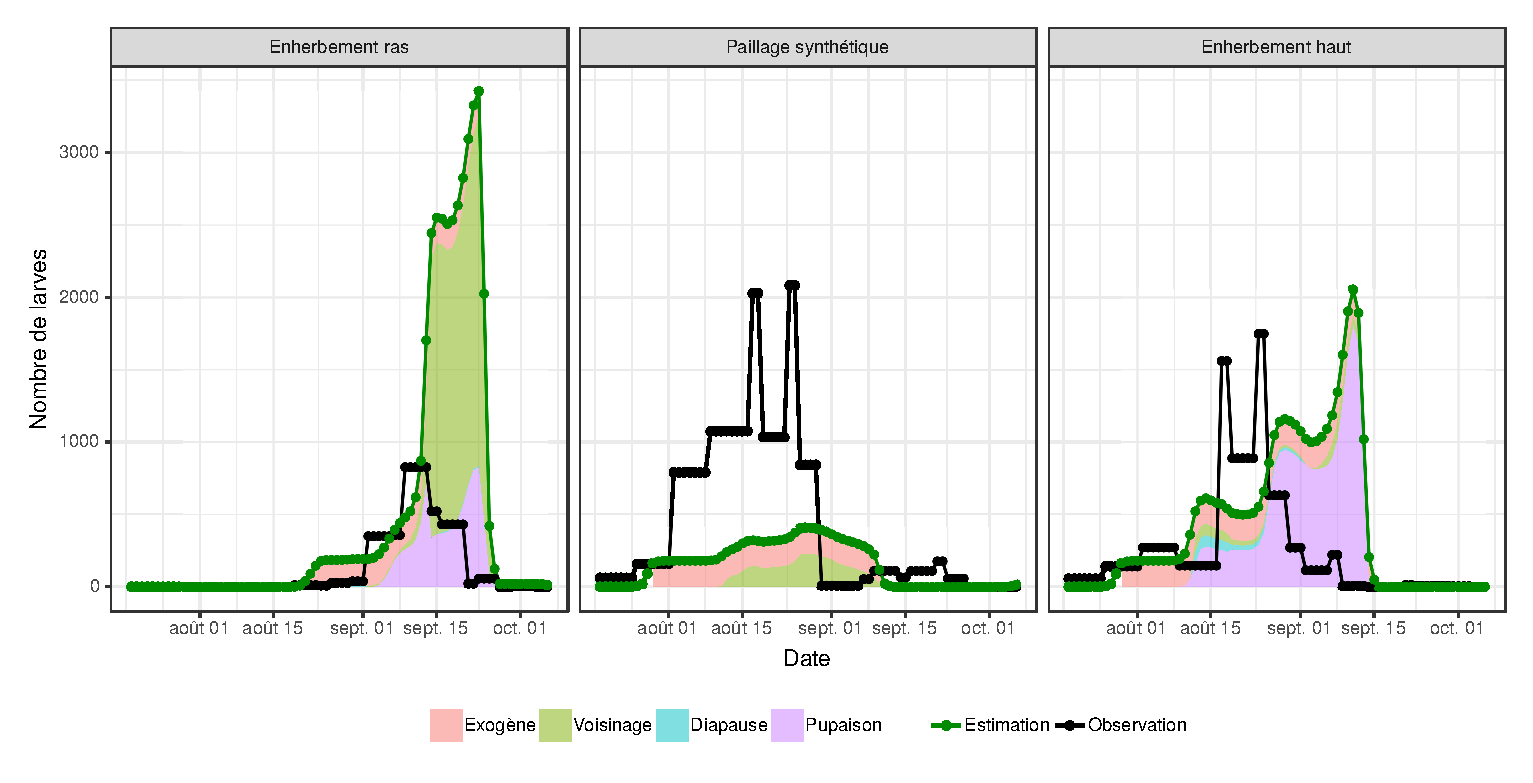
\epsfig{file = plots/verger2_15sept.eps, scale = 0.59}
 \caption{Dynamiques observées et simulées sur le verger n\textdegree2. La décomposition indiquant la provenance des femelles qui ont pondus les œufs est disponible pour les dynamiques simulées.
 Les paramètres utilisés sont ceux calibrés par le modèle sur le verger n\textdegree1.}
 \label{fig:vg2_15s}
\end{figure}


On pourrait cependant objecter que le phénomène de saisonnalité intervient à une autre date sur ce verger, les conditions climatiques pouvant être différentes.
En se basant sur les dynamiques observées, il semble que le phénomène de saisonnalité a lieu sur ce verger aux alentours du 23 août pour les modalités PS et EH et aux alentours du 7 septembre pour la modalité ER.

Les résultats produits sur le verger n\textdegree2 sont visibles sur la figure~\ref{fig:D2}.
On remarque que les dynamiques des modalités ER et EH sont plus ou moins captées.
En revanche, si la temporalité de la dynamique de la sous-parcelle PS semble correcte, son intensité n'est pas restituée correctement.
\begin{figure}[ht]
 \centering
 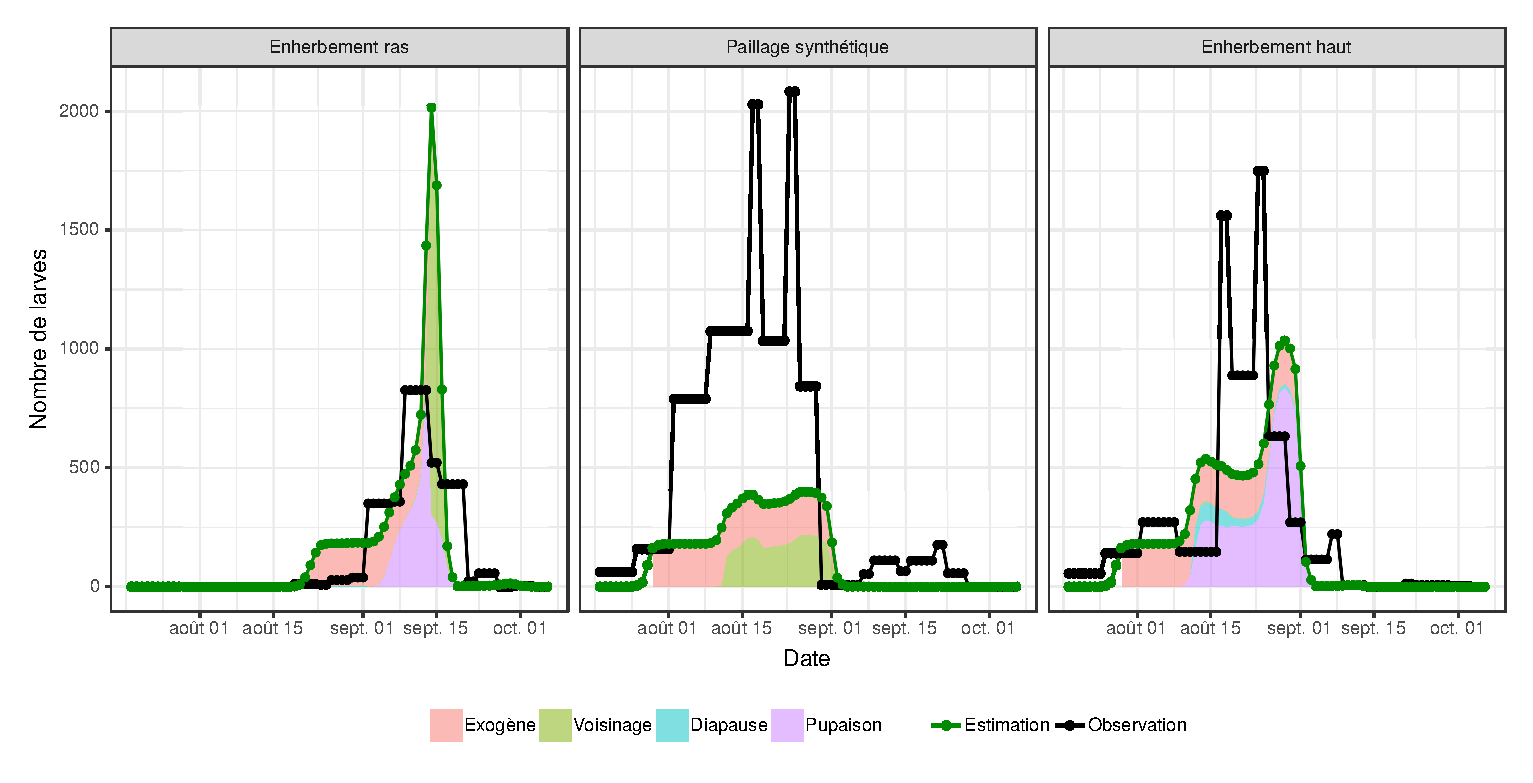
\epsfig{file = plots/D_b2.eps, scale = 0.59}
 \caption{Dynamiques observées et simulées sur le verger n\textdegree2. La décomposition indiquant la provenance des femelles qui ont pondus les œufs est disponible pour les dynamiques simulées.
 Les paramètres utilisés sont ceux calibrés par le modèle sur le verger n\textdegree1.}
 \label{fig:D2}
\end{figure}



% Le fait que les paramètres trouvés par le modèle en calibrant sur le verger n\textdegree1 ne s'applique pas au verger n\textdegree2 peut s'expliquer par la forte variabilité du phénomène observé.
% En effet, si l'une des deux dynamiques observées est très atypiques par rapport au comportement moyen, 










% Chapitre 7
\chapter{Conclusion} 

\lettrine{S}{i} l'on considère que l'objectif principal du stage était d'améliorer la compréhension du système manguier -- cécidomyies, alors le stage est une réussite.
Plus précisément, il y avait trois objectifs.

Le premier était de modéliser le système manguier -- cécidomyies des fleurs.
Le modèle existe et il est fonctionnel.
Cet objectif est atteint.

Le deuxième objectif était d'analyser le fonctionnement dudit système.
Les grandes composantes du système ont été identifiés et modélisées.
On n'a cependant validé que partiellement les paramètres sur le verger n\textdegree2.
Il est important de noter que le modèle fait une prédiction et semble mettre en évidence l'existence d'un phénomène en fin de saison, jusqu'alors non identifié, responsable de la diminution du nombre de cécidomyies --- ce qui permet d'envisager de nouvelles pistes pour mieux comprendre le système.

Le troisième objectif était de réaliser des tests \emph{in silico} afin d'évaluer le meilleur mode de gestion des vergers.
Cet objectif était conditionné aux deux autres.
Bien que la finalisation du modèle a pris du temps, la dernière version du modèle doit permettre de faire une telle analyse dans le futur.
% Et le deuxième objectif a mis en évidence qu'il nous manquait des connaissances dans la compréhension du système, rendant les simulations \emph{in silico} peu pertinentes.

À l'issue de ce stage, on peut envisager plusieurs pistes pour de futures améliorations.
Par exemple, réaliser de nouvelles expérimentations sur le terrain pour acquérir plus de données sur l'attractivité des différents stades phénologiques des inflorescences.
Et aussi s'intéresser à la possible compétition entre la cécidomyie des fleurs et d'autres ravageurs.
Il faudra \emph{a priori} acquérir plus de connaissances et/ou de données avant d'entreprendre à nouveau une démarche de modélisation.

\paragraph{ } D'un point de vue personnel, ce stage aura été une réussite.
D'abord d'un point de vue technique. J'ai pu appliquer des concepts mathématiques appris en cours à un cas concret.
J'ai aussi été amené à apprendre par moi-même des concepts non vus en cours relatifs à l'optimisation et l'analyse de sensibilité d'un modèle, et à les appliquer. Cela fut très intéressant.

Ensuite d'un point de vue professionnel, j'ai pu avoir une première expérience dans le domaine de la recherche.
Expérience fort plaisante, qui m'a permis de me faire une idée plus précise du métier de chercheur.
Et de rappeler certaines évidences : les résultats obtenus ne sont pas toujours ceux que l'on cherche initialement, et que cette incertitude est au cœur même du métier.
Et c'est ce qui rend ce métier passionnant.


\bibliography{biblio}

\end{document}

